\documentclass[a4paper,utf8]{article}
\usepackage[heading,fancyhdr]{ctex}
\usepackage{amsmath,amssymb,geometry,lastpage,ulem}
\usepackage{array,tabularx,graphicx,floatrow}
\geometry{
    top=25.4mm, 
    left=30mm, 
    right=30mm, 
    bottom=35mm,
    headsep=5.9mm,
}
\ctexset{
    section = {format+=\raggedright}
}
\newcommand{\expinfo}[5]{
    {\zihao{-3}\bfseries\songti
    实验名称:\uline{\hfill\mbox{#1}\hfill} \\[2.9mm]
    学\quad 号:\uline{\makebox[25mm]{#2}}\hfill
    姓\quad 名:\uline{\makebox[25mm]{#3}}\hfill
    班\quad 级:\uline{\makebox[25mm]{#4}} \\[2.9mm]
    合作者:\uline{\makebox[25mm]{无}}\enspace~
    桌\quad号:\uline{\makebox[25mm]{}}\hfill\mbox{}\\[2.9mm]
    指导教师:\uline{\makebox[30mm]{#5}}\hfill\mbox{} \\[2.9mm]
    实验日期:\uline{\makebox[30mm]{}}\hfill\mbox{} \\[58.7mm]
    }
}%\expinfo{实验名称}{学号}{姓名}{班级}{指导教师}
\pagestyle{fancy}
\fancyhf{} \fancyhead[C]{材料科学基础实验} \fancyfoot[C]{\thepage~/~\pageref{LastPage}}
\begin{document}
\begin{center}
    {\mbox{}\\[7em]\zihao{2}\bfseries\songti%
    材料科学基础实验报告}\\[34mm]
    \expinfo{实验一 铁碳合金的显微组织观察及性能分析}{22301070}{杨雨燃}{22材物}{杨玉华}
    {\zihao{4}\bfseries\songti
    实验考核\\[3mm]
    \extrarowheight=3mm
    \begin{tabularx}{150mm}{|X|X|X|X|X|}\hline
        \hfil 项目 \hfil  & \hfil 实验预习 \hfil & \hfil 实验过程 \hfil & \hfil 分析与讨论 \hfil & \hfil 总评 \hfil \\[3mm] \hline
        \hfil 评价 \hfil &  &  &  &  \\[3mm] \hline
    \end{tabularx}
    }
\end{center}

\newpage
\section*{【实验目的】}
    \begin{enumerate}
        \item 了解金相显微镜的成像基本原理、构造、主要部件及作用;
        \item 熟悉金相显微镜的使用和其注意事项;
        \item 掌握分析铁碳合金在平衡状态下及不同工艺热处理后的显微组织形态;
        \item 加深理解铁碳合金组织与性能之间的关系。
    \end{enumerate}   
\section*{【实验原理】}%简单描述,含必要的公式和附图;
    \begin{enumerate}
        \item 金相分析是研究材料内部组织和缺陷的主要方法之一,是研究金属材料微观结构最基本的一种实验技术。通过显微分析可以研究材料内部的组织与其化学成分的关系;确定各类材料经不同方式加工及热处理后的显微组织;判断材料质量的优劣,如金属材料中诸如氧化物、硫化物等各种非金属夹杂物在显微组织中的大小、数量、分布情况以及晶粒度的大小等。
        \item 金相显微镜的成像原理如图:
        
        \begin{center}
            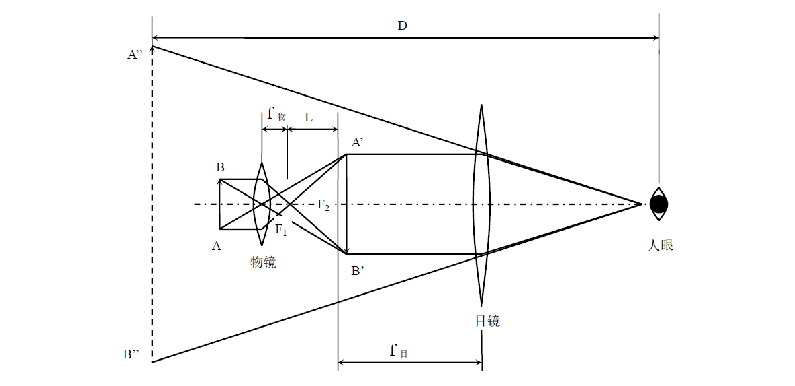
\includegraphics[width=300pt]{1.png}
        \end{center}
        
        显微镜的放大倍数为:
                       $M = M_\text{物} * M_\text{目}$
        \item 金相显微镜的主要性能参数:
        \item 
        ①物镜的数值孔径
        
        ②分辨率(横向分辨率)

        ③焦深(垂直分辨率)
        \item 金相显微镜的构造:
        \begin{center}
            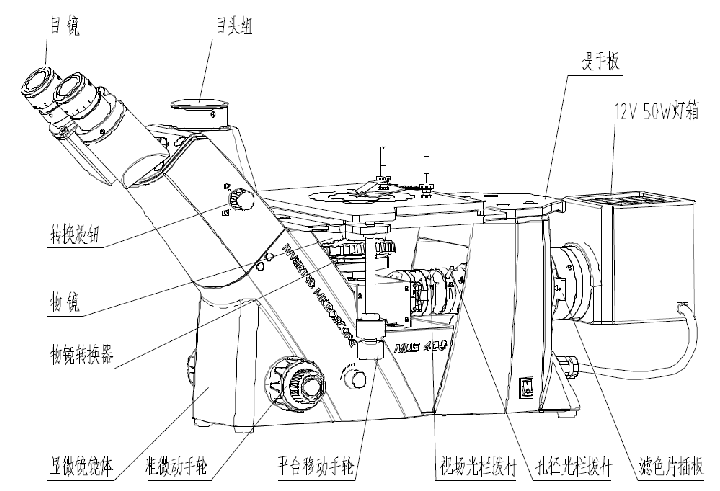
\includegraphics[width=400pt]{2.png} 
        \end{center}
        \item 七种典型铁碳合金:

    ①工业纯铁:含碳量小于0.0218\%,室温下显微组织由白色块状铁素体和极少量三次渗碳体(通常可忽略)构成。用硝酸酒精浸蚀后显微组织呈白色多边形,晶界呈黑色网状

    ②亚共析钢:含碳量为0.0218\%~0.77\%,在显微镜下观察时,若珠光体的层片间距较大或者放大倍数较高时其呈片层状,且可清楚地看到珠光体中平行相间的宽条铁素体和细条渗碳体;若珠光体在层片间距较小或者放大倍数较低时,则其片层结构不能分辨,呈暗黑色。另随着含碳量的增加,珠光体含量增加,铁素体含量减少。
    
    ③共析钢:含碳量为0.77\%,室温下的显微组织全部由层片状珠光体(P)组织构成,即片状铁素体和渗碳体的机械混合物,且铁素体与渗碳体质量比约为7.9:1,铁素体厚,渗碳体薄。用硝酸酒精浸蚀后,珠光体中铁素体与渗碳体都呈白亮色,只有相界呈黑色。
    
    ④过共析钢:含碳量为0.77\%~2.11\%,室温下的显微组织由白亮色网状二次渗碳体和层片状珠光体(P)构成。用硝酸酒精浸蚀后,二次渗碳体成亮白色网分布在珠光体的周围。
    
    ⑤亚共晶白口铸铁:含碳量为2.11\%~4.3\%,室温下的显微组织由黑色树枝状珠光体(P)、二次渗碳体和豹皮状低温莱氏体构成,二次渗碳体在珠光体周围析出,与莱氏体中的渗碳体连在一起,难以分辨。
    
    ⑥共晶白口铸铁:含碳量为4.3\%,室温下的显微组织由豹皮状低温莱氏体构成,其中白色集体为共晶渗碳体,黑色粒状或棒状组织为珠光体,其片层状无法分辨而成黑色。
    
    ⑦过共晶白口铸铁:含碳量为4.3\%~6.69\%,室温下的显微组织由一次渗碳体和低温莱氏体构成,其中的一次渗碳体呈白亮色板条状分布在低温莱氏体中。
    \end{enumerate}



\section*{【实验仪器】}%规格及参数
1、MDS400倒置式金相显微镜

2、铁碳合金平衡状态金相试样×1,多种热处理方式之后的碳钢式样×1
\section*{【实验过程】}%简述主要过程和实验内容

1. 领取一套经不同热处理工艺的45钢及T12钢标准试样(21\#-27\#),在显微镜下观察经
不同热处理工艺的45钢及T12试样。理解并分析不同热处理工艺条件下试样的组织变化,认
真体会整个操作过程,并将观察图像拍照存储。
其中:
21\#为45钢860℃水淬+中温回火;
22\#为45钢860℃水淬+高温回火;
23\#为45钢780℃水淬;
24\#为45钢1100℃水淬;
25\#为T12钢球化退火;
26\#为T12钢780℃水淬+低温回火;
27\#为T12钢1100℃水淬+低温回火。

2.注意事项:
1、操作时必须特别谨慎,不能有任何剧烈的动作,不允许自行拆卸光学系统。

2、在旋转粗调或微调旋钮时动作要慢,碰到某种障碍时应立即停止操作,报告指导教师查找
原因,不得用力强行转动,否则会损坏机件。

3、要爱护已制备好的金相试样。不能用手触摸试样的观察面,如有尘埃等脏物不能用嘴吹,
也不能随意擦,要用吸耳球吹除或用无水酒精冲洗并干燥。

4、试样观察完毕后要放入干燥箱中保存。

\section*{【实验数据】}

1.纯铁

如图一图二,显微结构呈现规则的区块状铁素体,黑色的部分为晶界,将不同的铁素体隔开,使得界限较为分明,
其中在铁素体上,有分布一些颗粒状的渗碳体,其中,渗碳体分布不多。用硝酸酒精浸蚀后,显微组织
特征呈白色多边形晶粒,晶界呈黑色网络状。
\begin{figure}[!ht]
    \begin{floatrow}
        \ffigbox[50mm]{\caption{01-工业纯铁-200}}{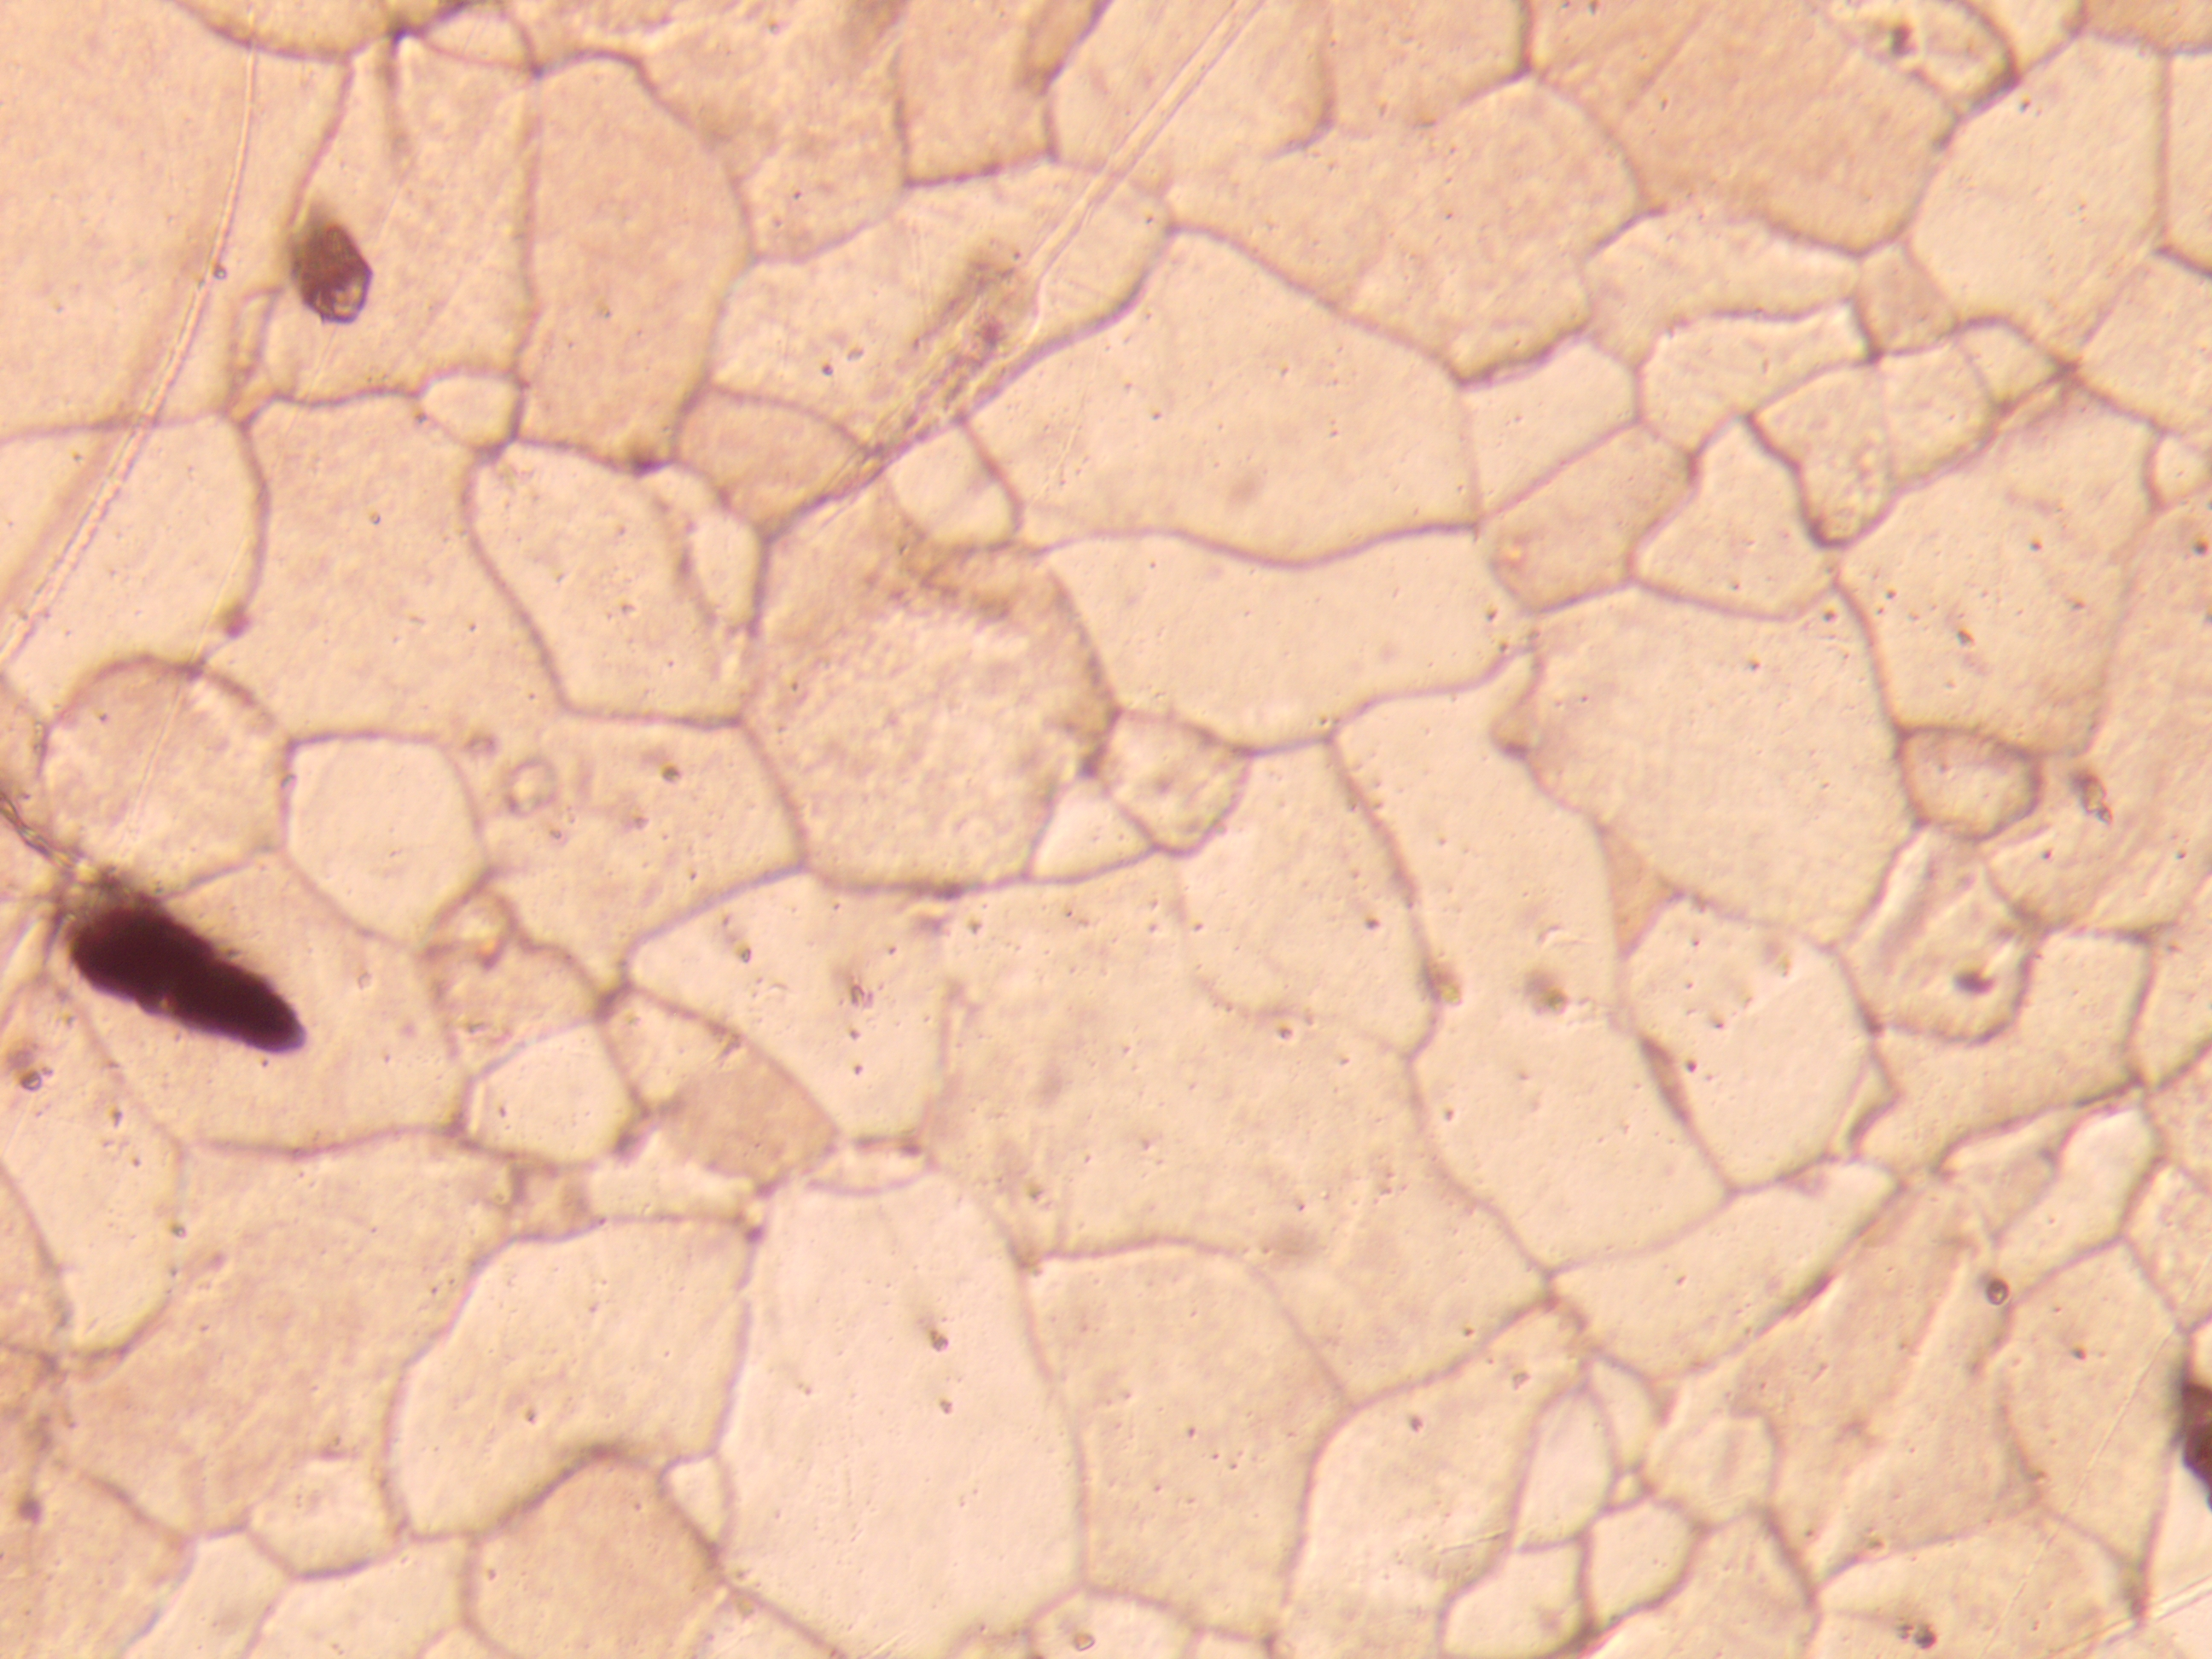
\includegraphics[width=50mm]{01-200.jpg}}
        \ffigbox[50mm]{\caption{01-工业纯铁-500}}{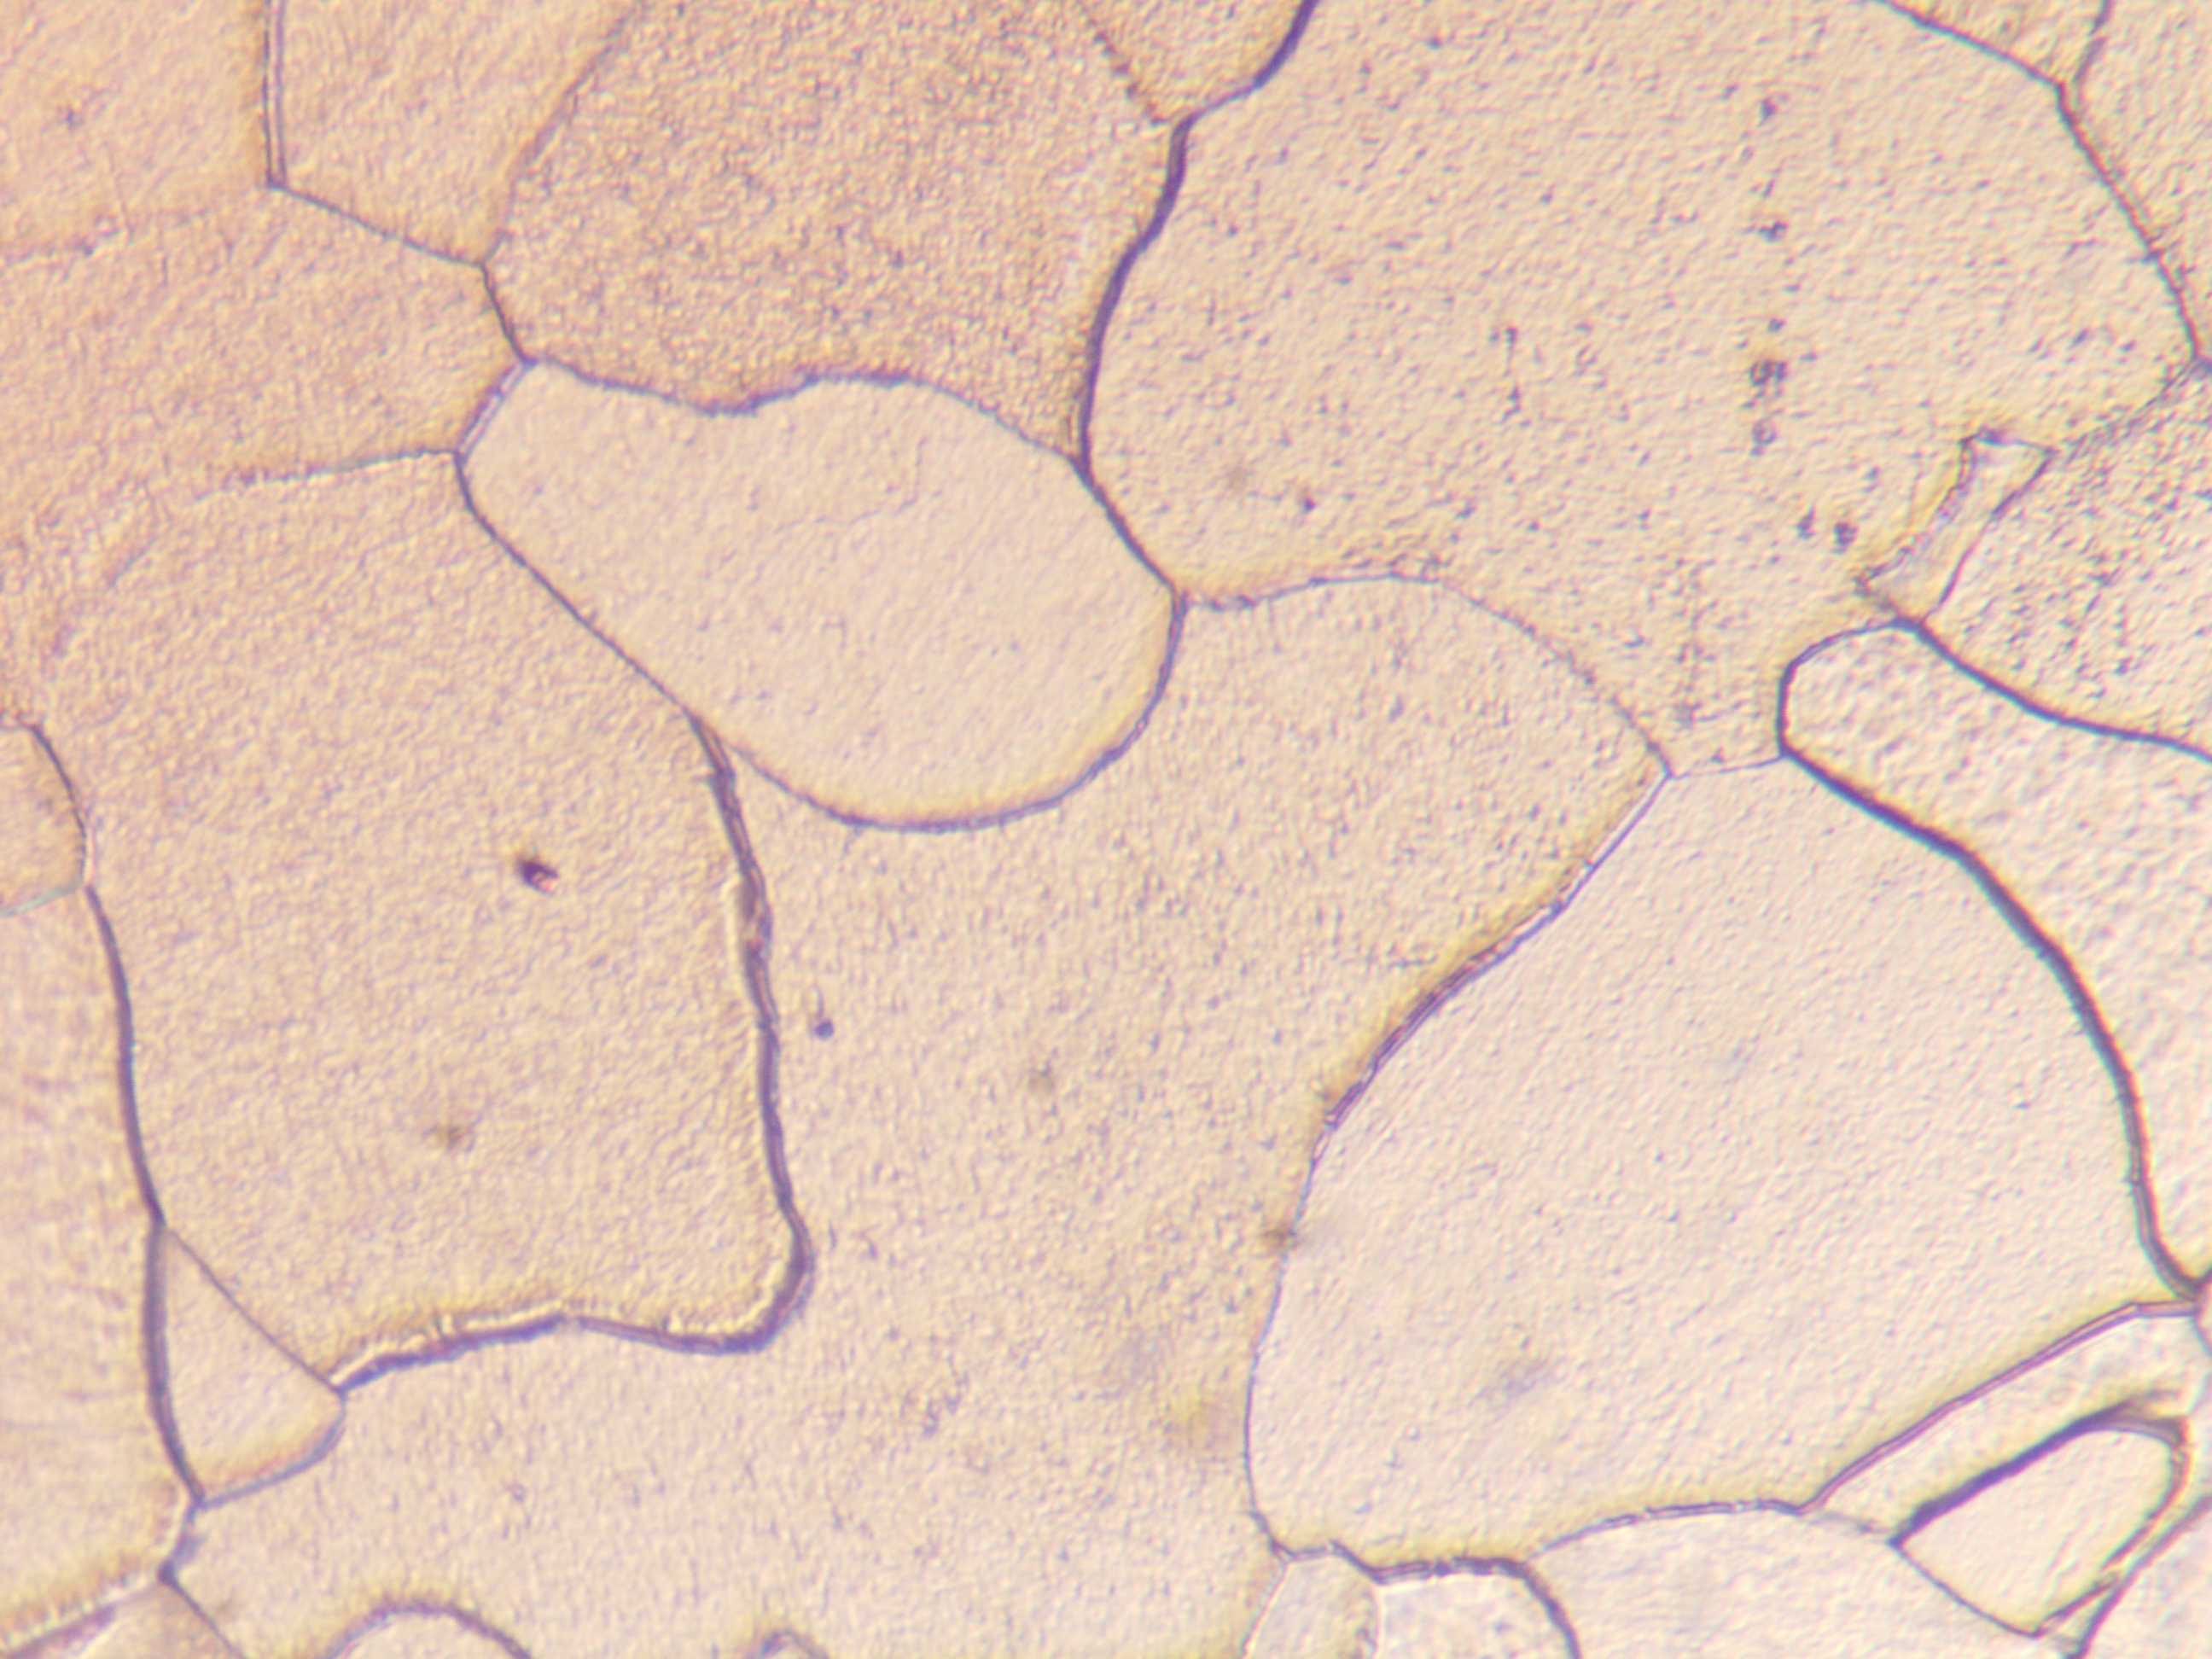
\includegraphics[width=50mm]{01-500.jpg}}
        \ffigbox[50mm]{\caption{01-工业纯铁}}{
\includegraphics[width=50mm]{5.png}}
    \end{floatrow}

\end{figure}

\newpage
2.45钢

如图三图四,显微结构下白色部分为铁素体,黑色(深色)部分为片状的珠光体,白色块状铁素体(F)和黑色的片状珠光体(P)交替分布,黑色网络为晶界。
随着含碳量的增加,铁素体含量减少同时珠光体含量增加。两者相对量可由杠杆原理求出。
\begin{figure}[!ht]
    \begin{floatrow}
        \ffigbox[50mm]{\caption{03-45钢-200}}{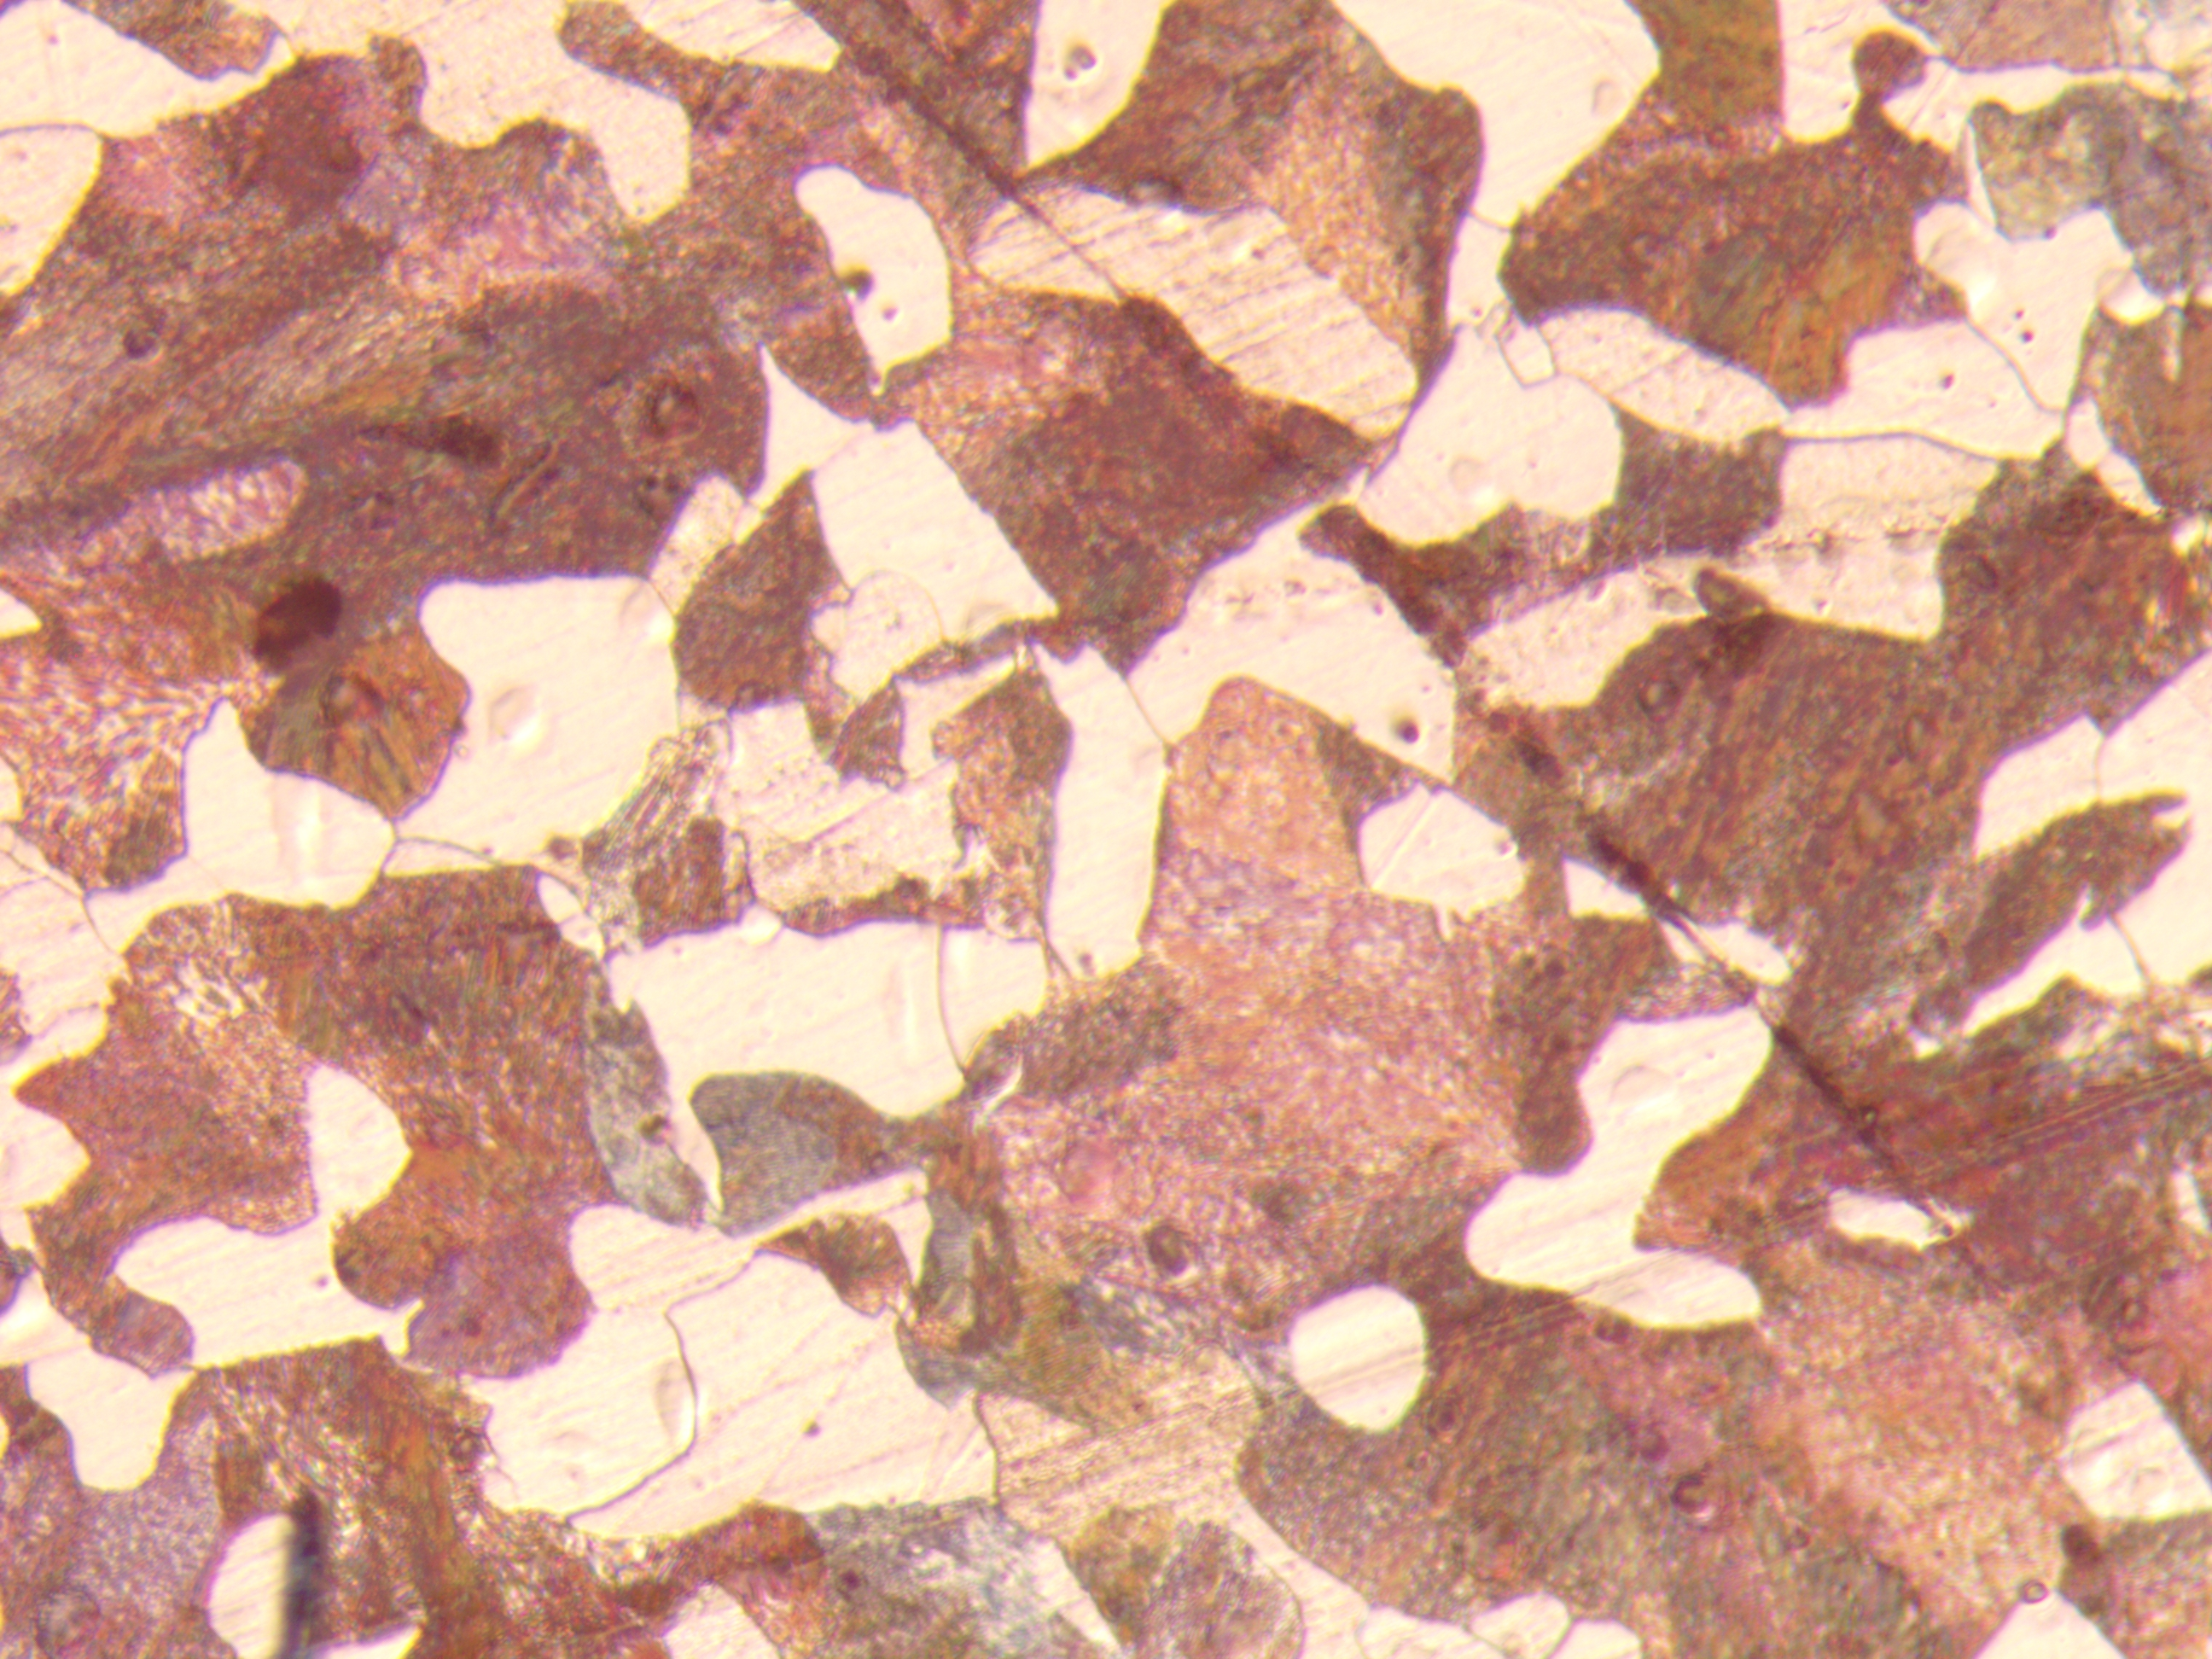
\includegraphics[width=50mm]{03-200.jpg}}
        \ffigbox[50mm]{\caption{03-45钢-500}}{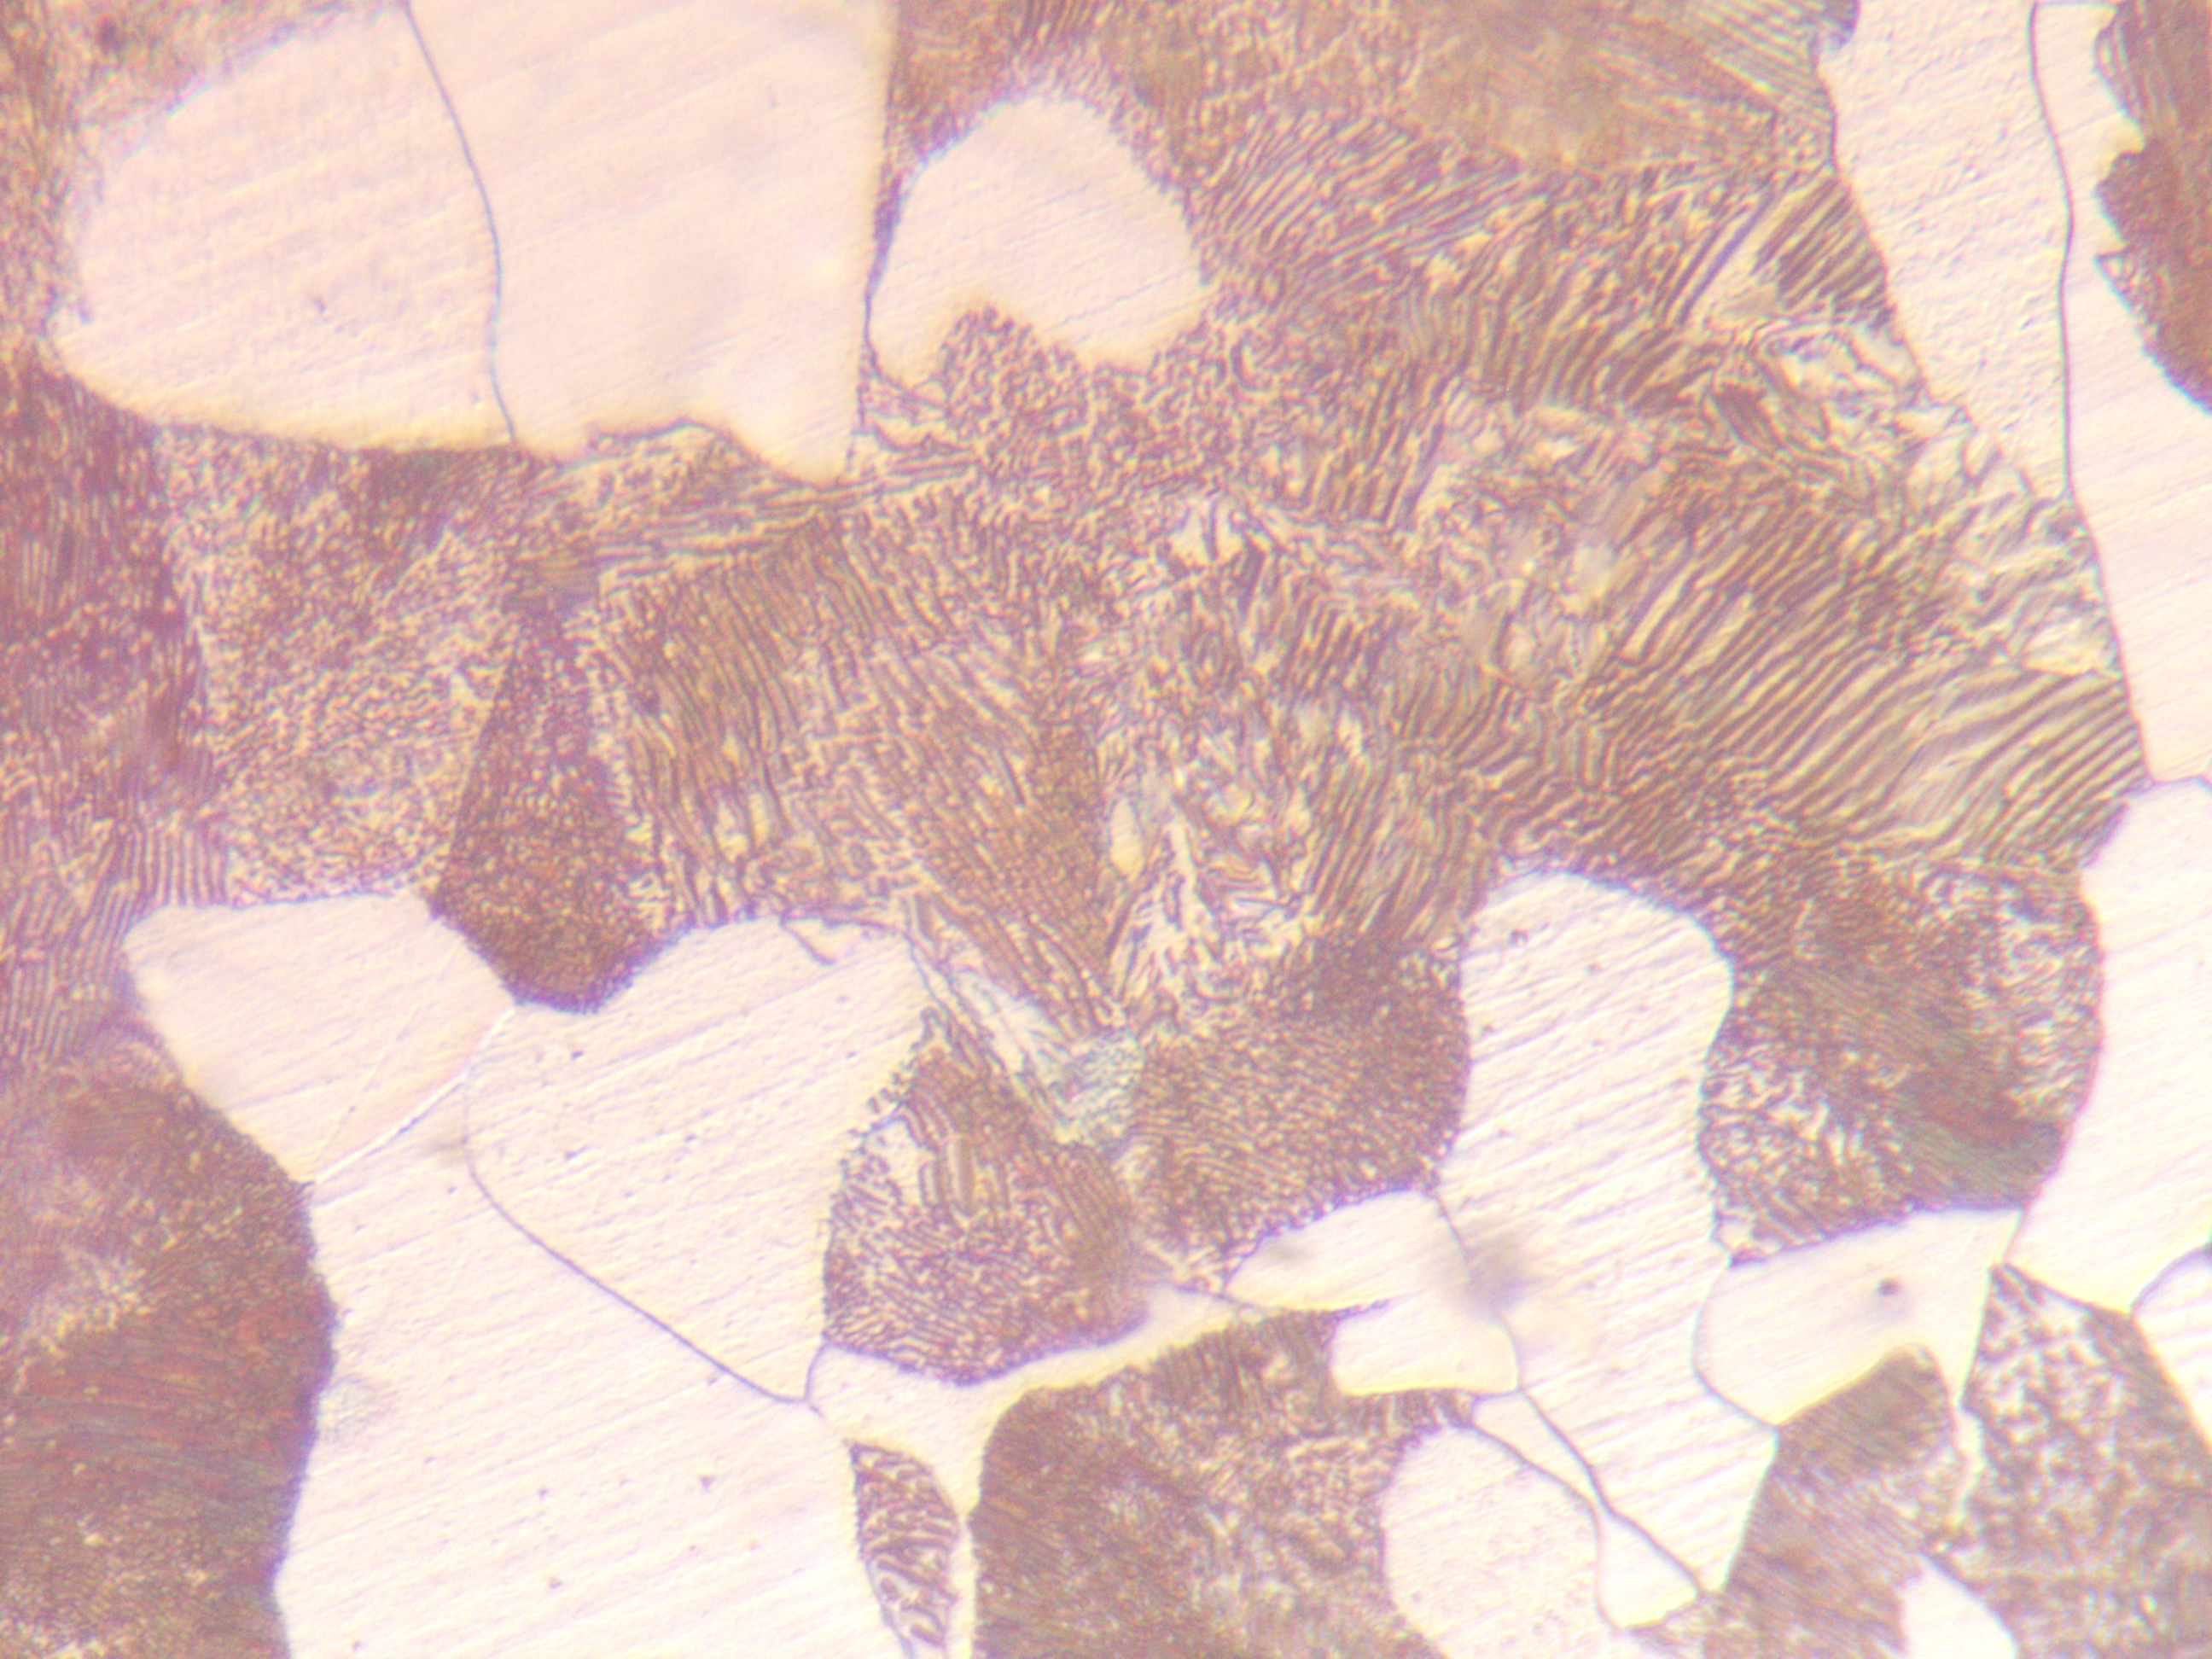
\includegraphics[width=50mm]{03-500.jpg}}
        \ffigbox[50mm]{\caption{03-45钢}}{
\includegraphics[width=50mm]{5.png}}
    \end{floatrow}

\end{figure}

3.T8钢

如图五图六,从200倍下观察可以知道,T8钢基本由片层状的珠光体构成,从500倍可知,其中由铁素体和渗碳体,
铁素体较宽,渗碳体比较细小,总体上细小的渗碳体呈现更深的颜色。
\begin{figure}[!ht]
    \begin{floatrow}
        \ffigbox[50mm]{\caption{05-T8钢-200}}{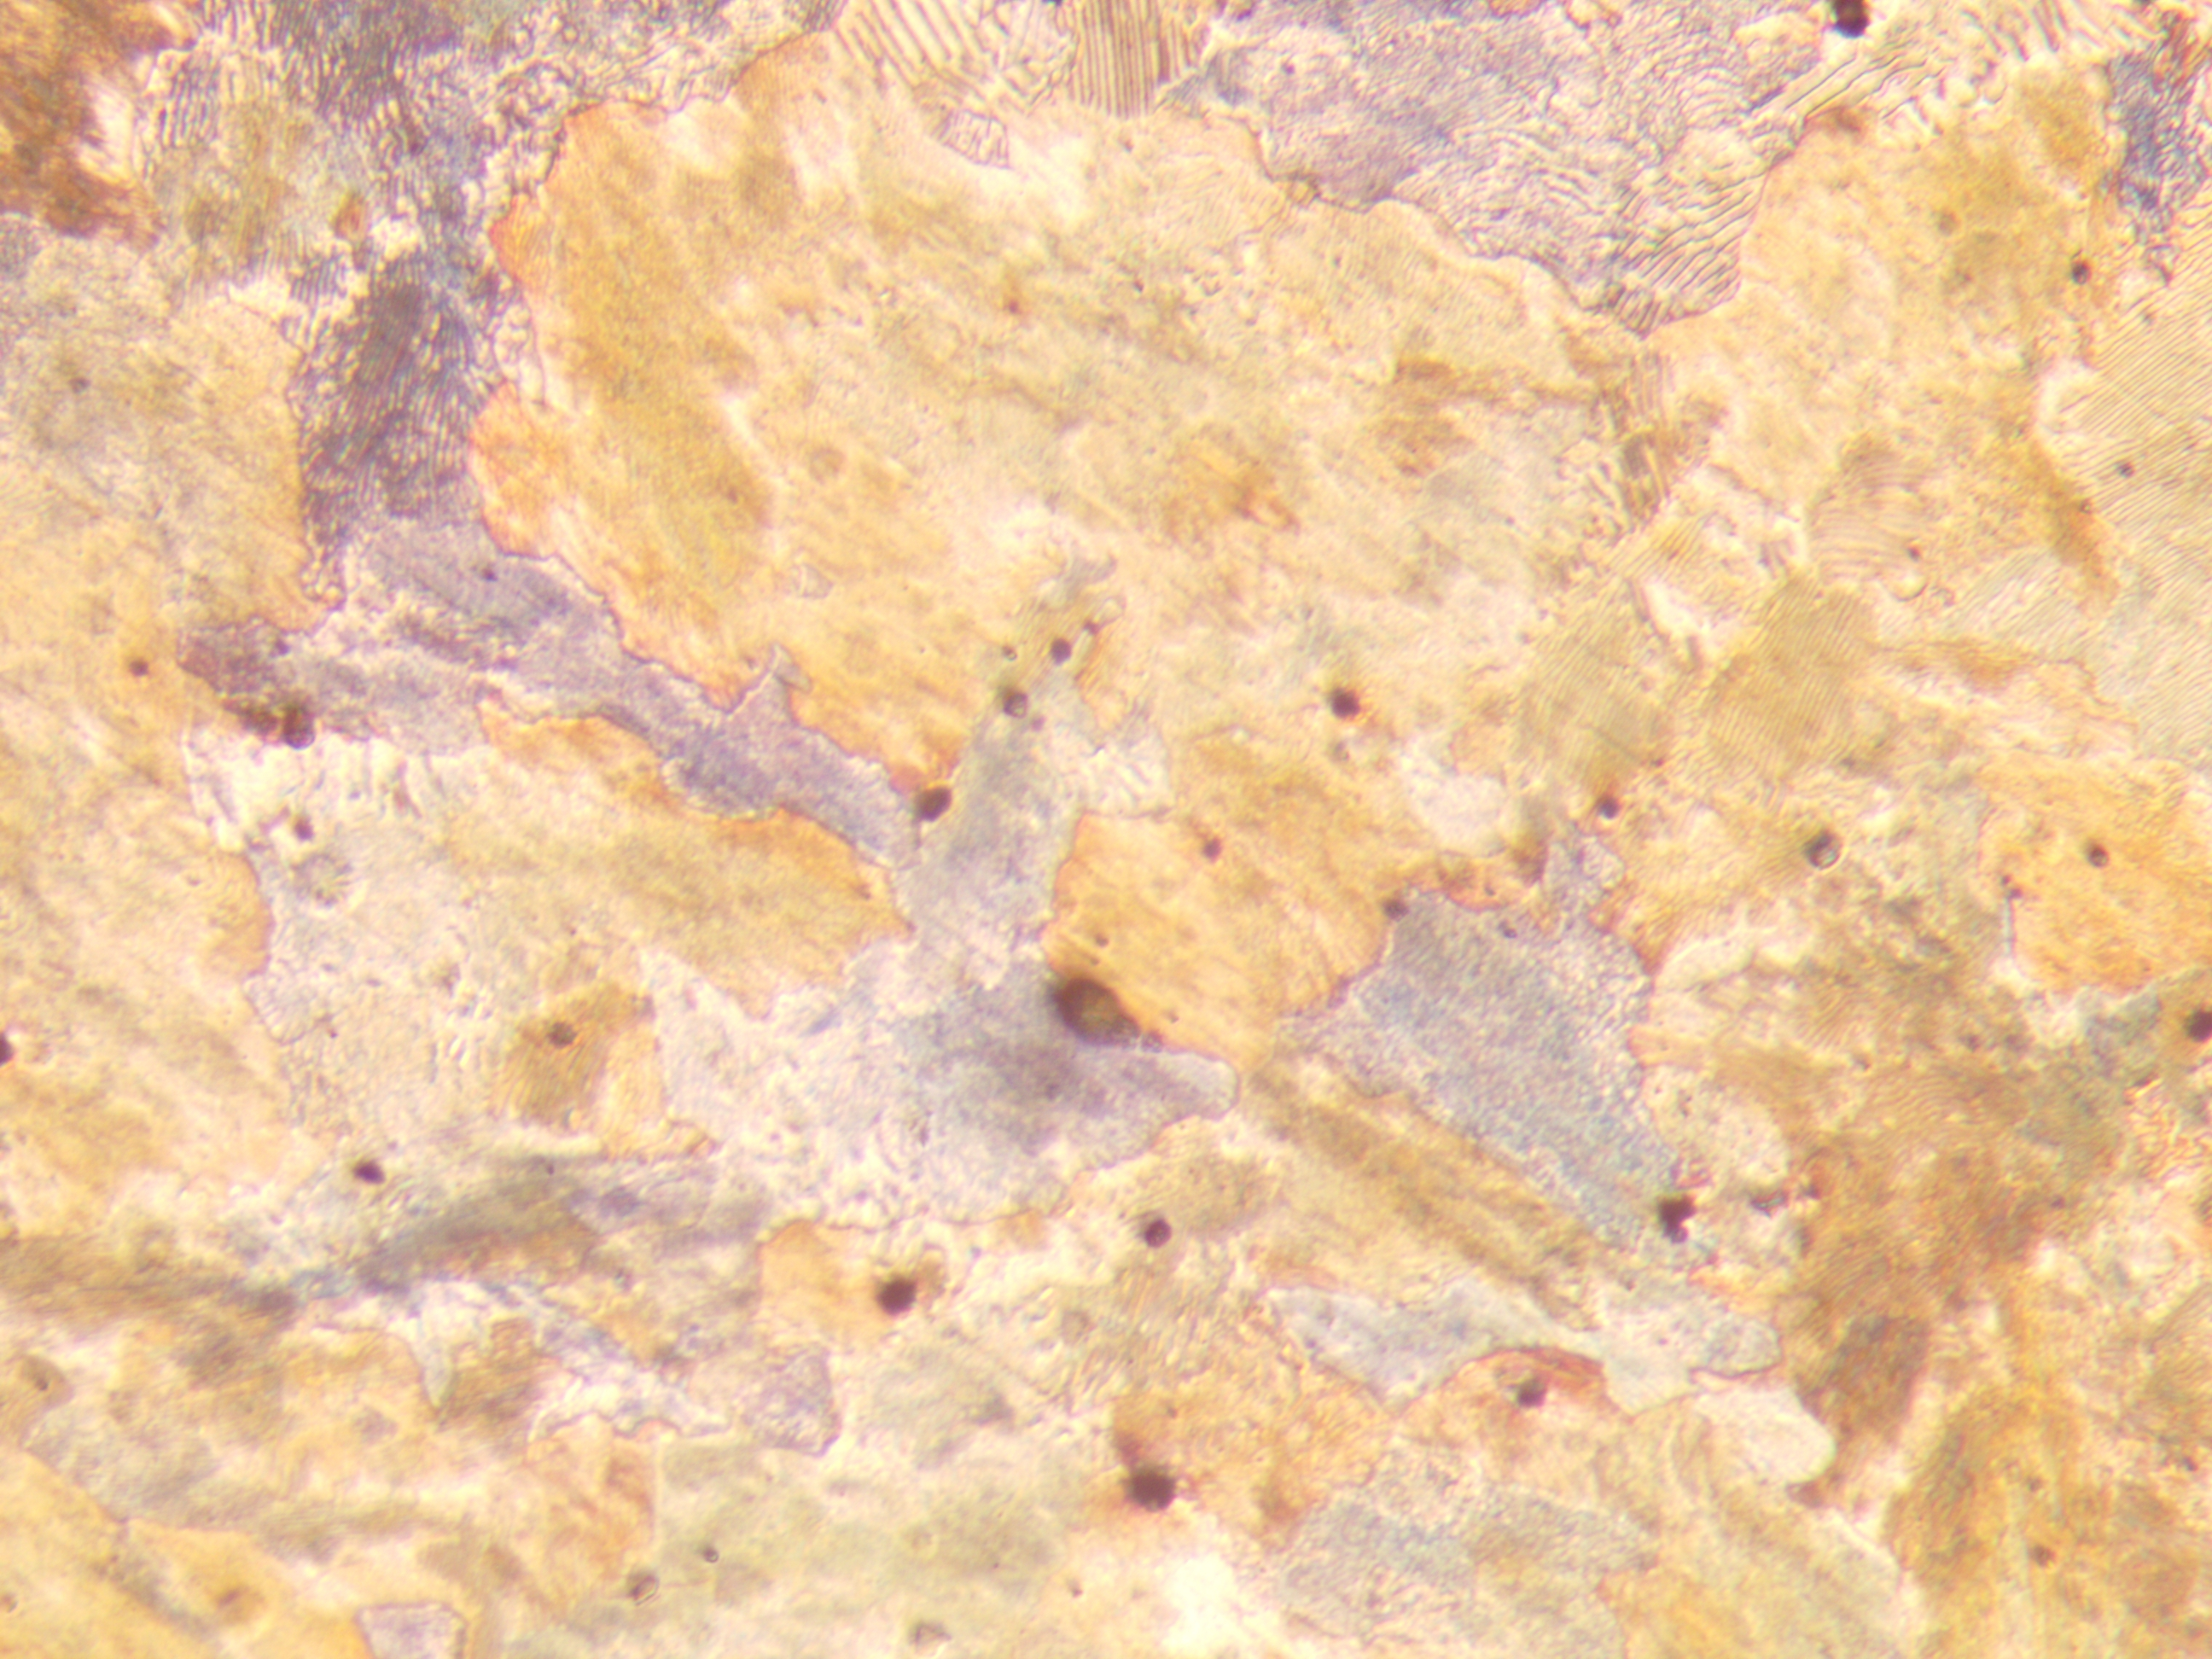
\includegraphics[width=50mm]{05-200.jpg}}
        \ffigbox[50mm]{\caption{05-T8钢-500}}{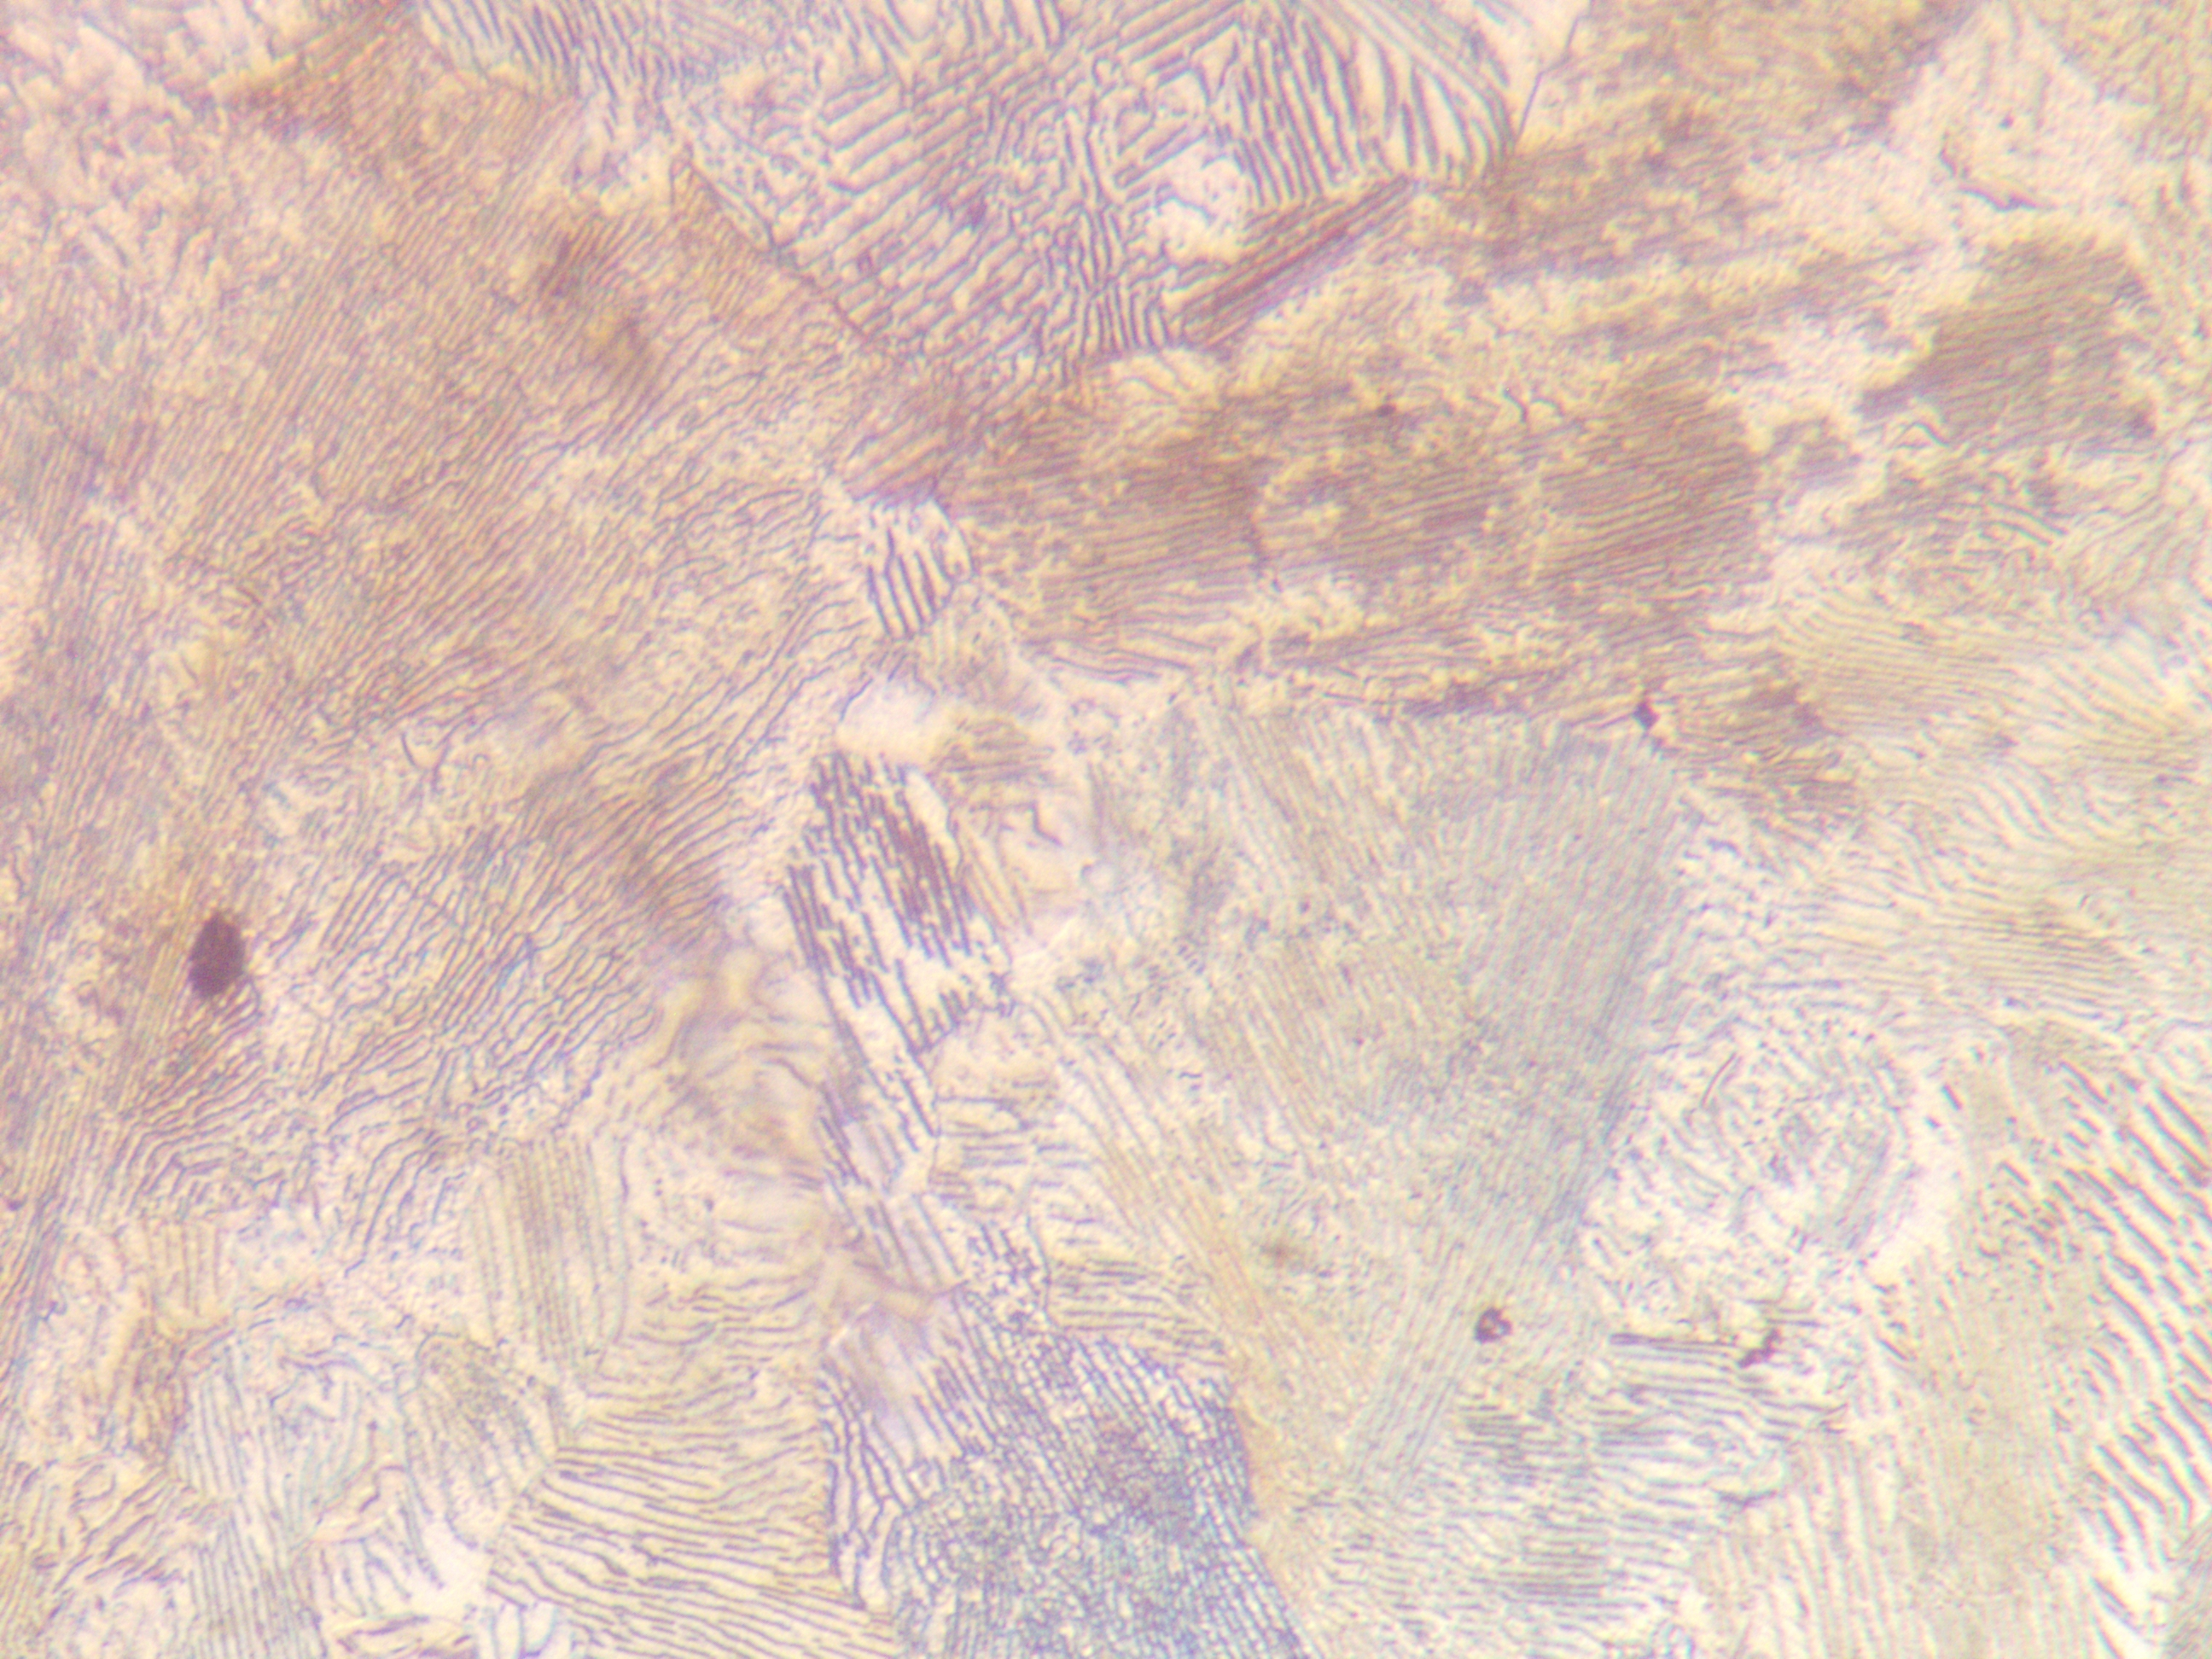
\includegraphics[width=50mm]{05-500.jpg}}
        \ffigbox[50mm]{\caption{05-T8钢}}{
\includegraphics[width=50mm]{5.png}}
    \end{floatrow}

\end{figure}

4.T12钢

如图七,图八,我们能从低倍镜下观察得到,T12钢的结构呈现一定程度的片层状,在白色围绕的部分内也有明显颜色深浅差异,
高倍数显微镜下能观察到区域化的层片状珠光体结构, 亮白色的部分是二次渗碳体,中间的渗碳体和铁素体较为细小,显现出颜色差异。
\begin{figure}[!ht]
    \begin{floatrow}
        \ffigbox[50mm]{\caption{06-T12钢-200}}{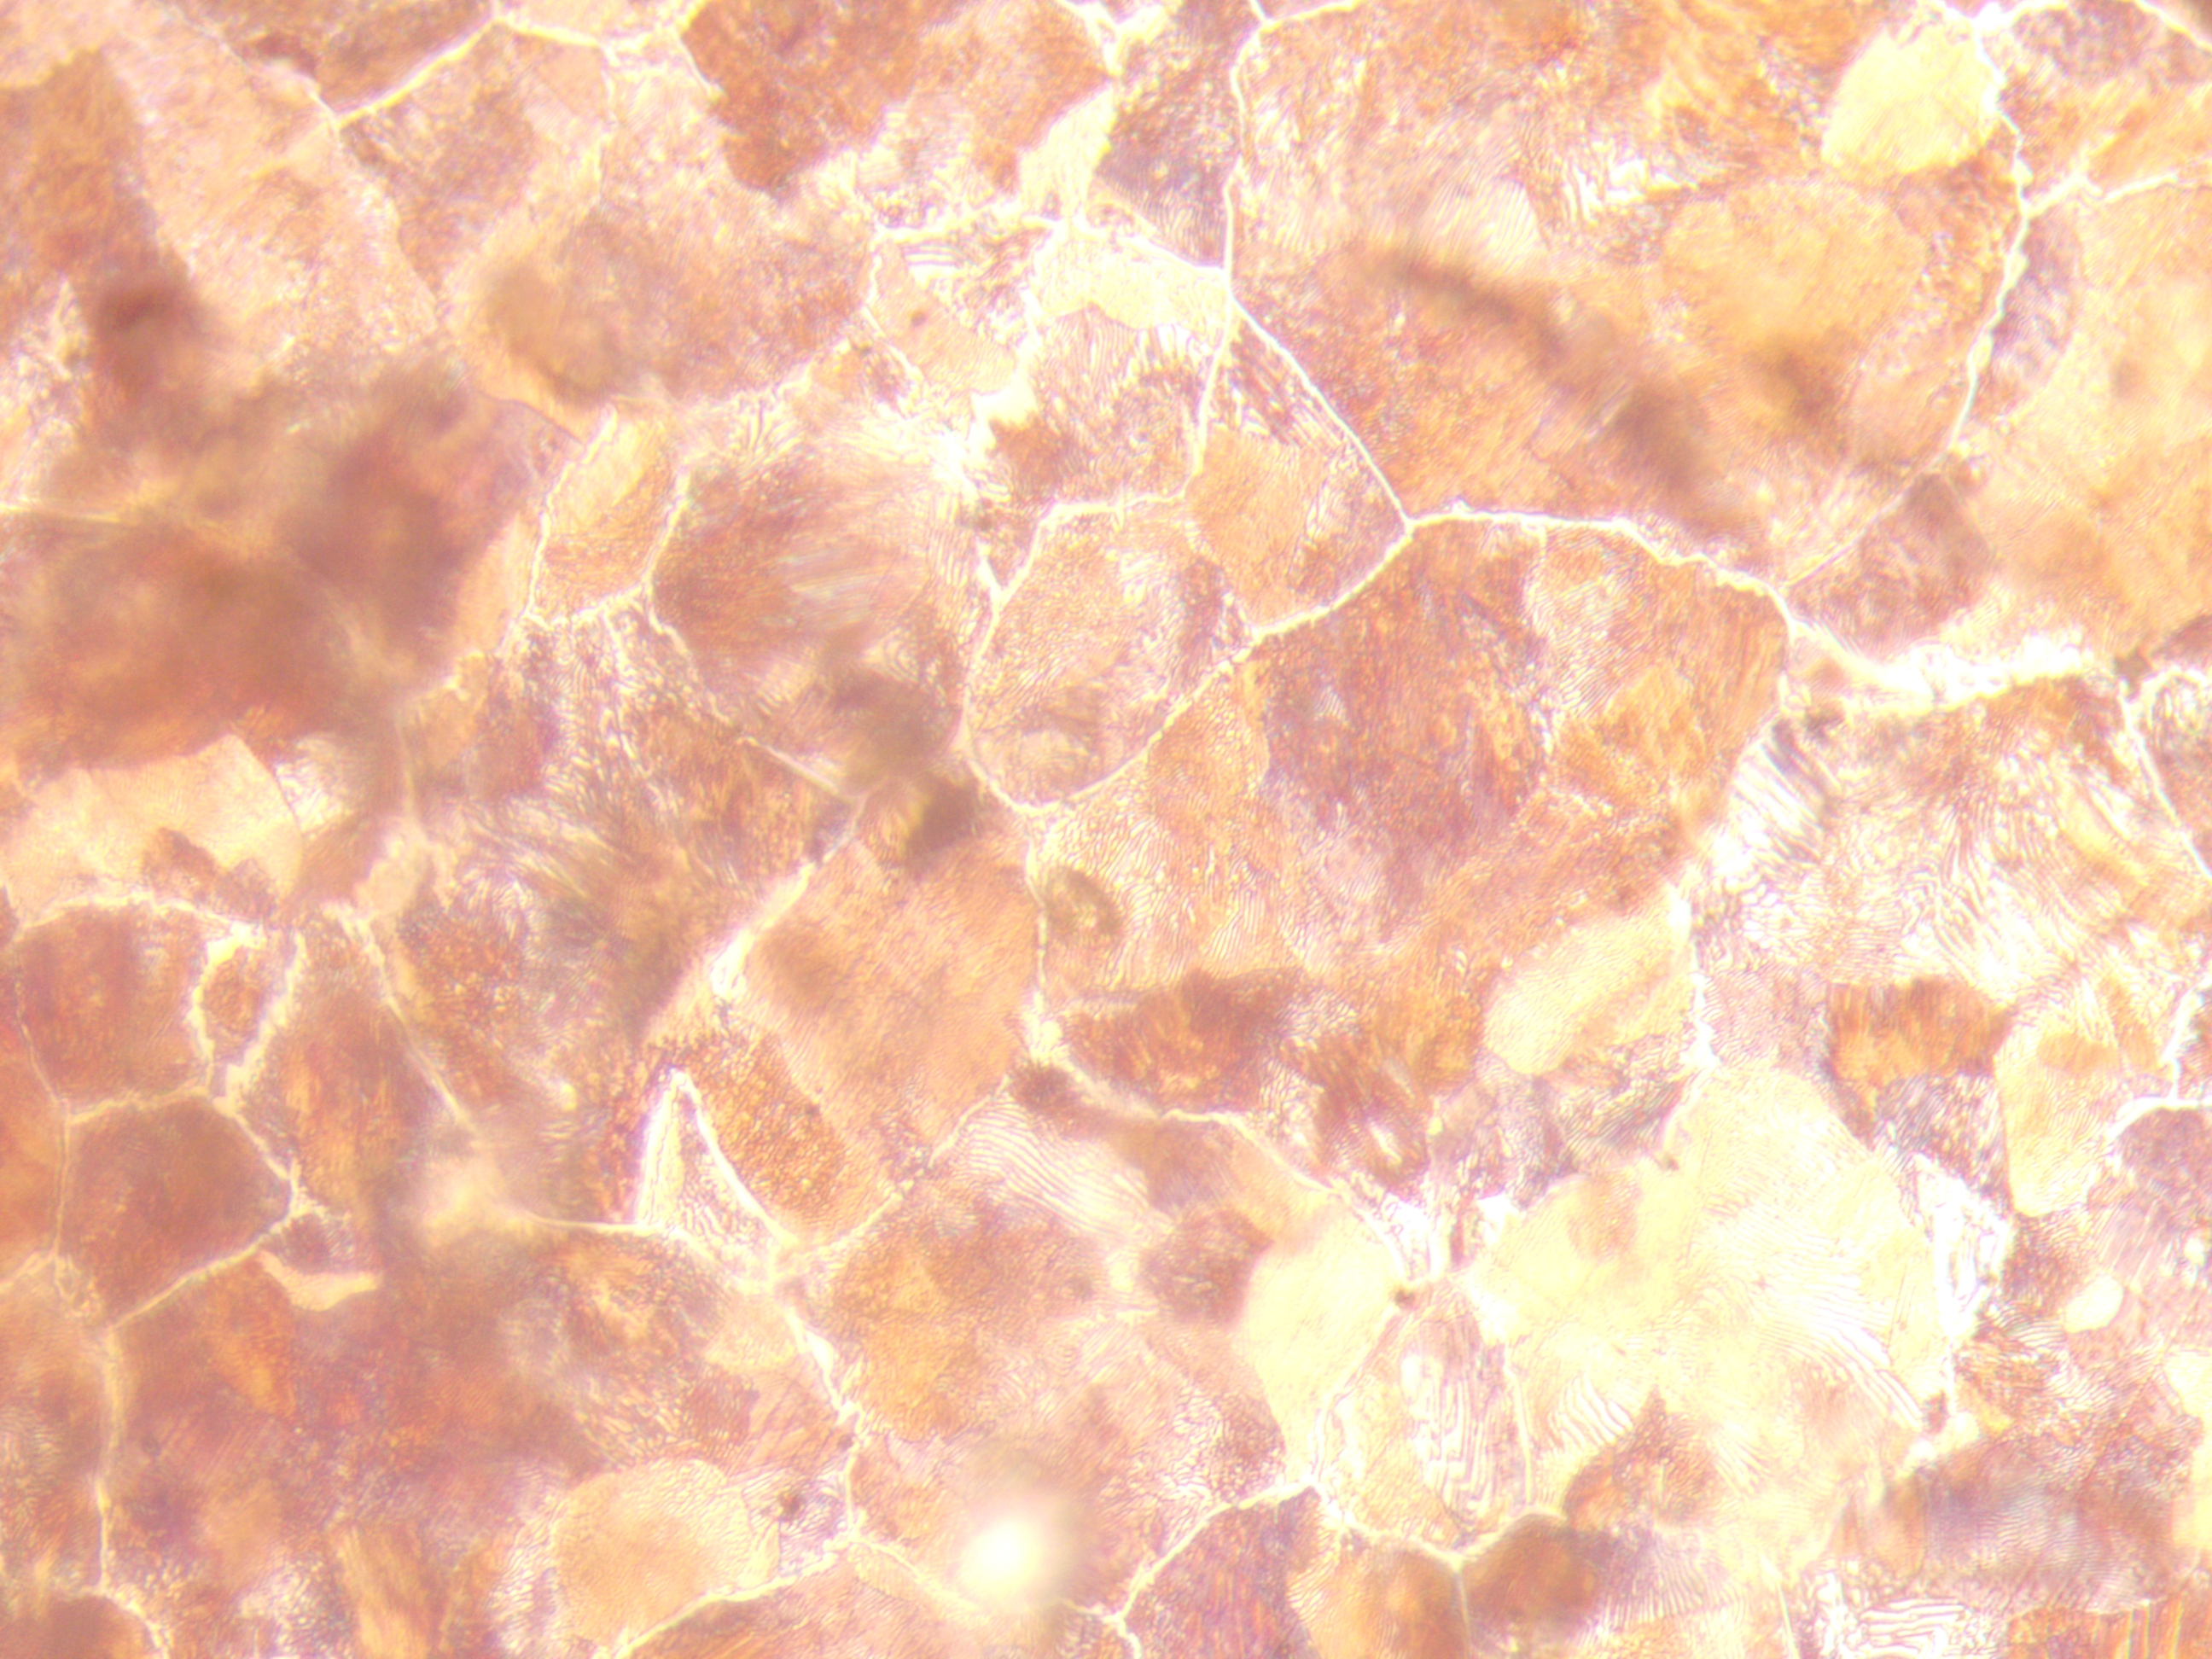
\includegraphics[width=50mm]{06-200.jpg}}
        \ffigbox[50mm]{\caption{06-T12钢-500}}{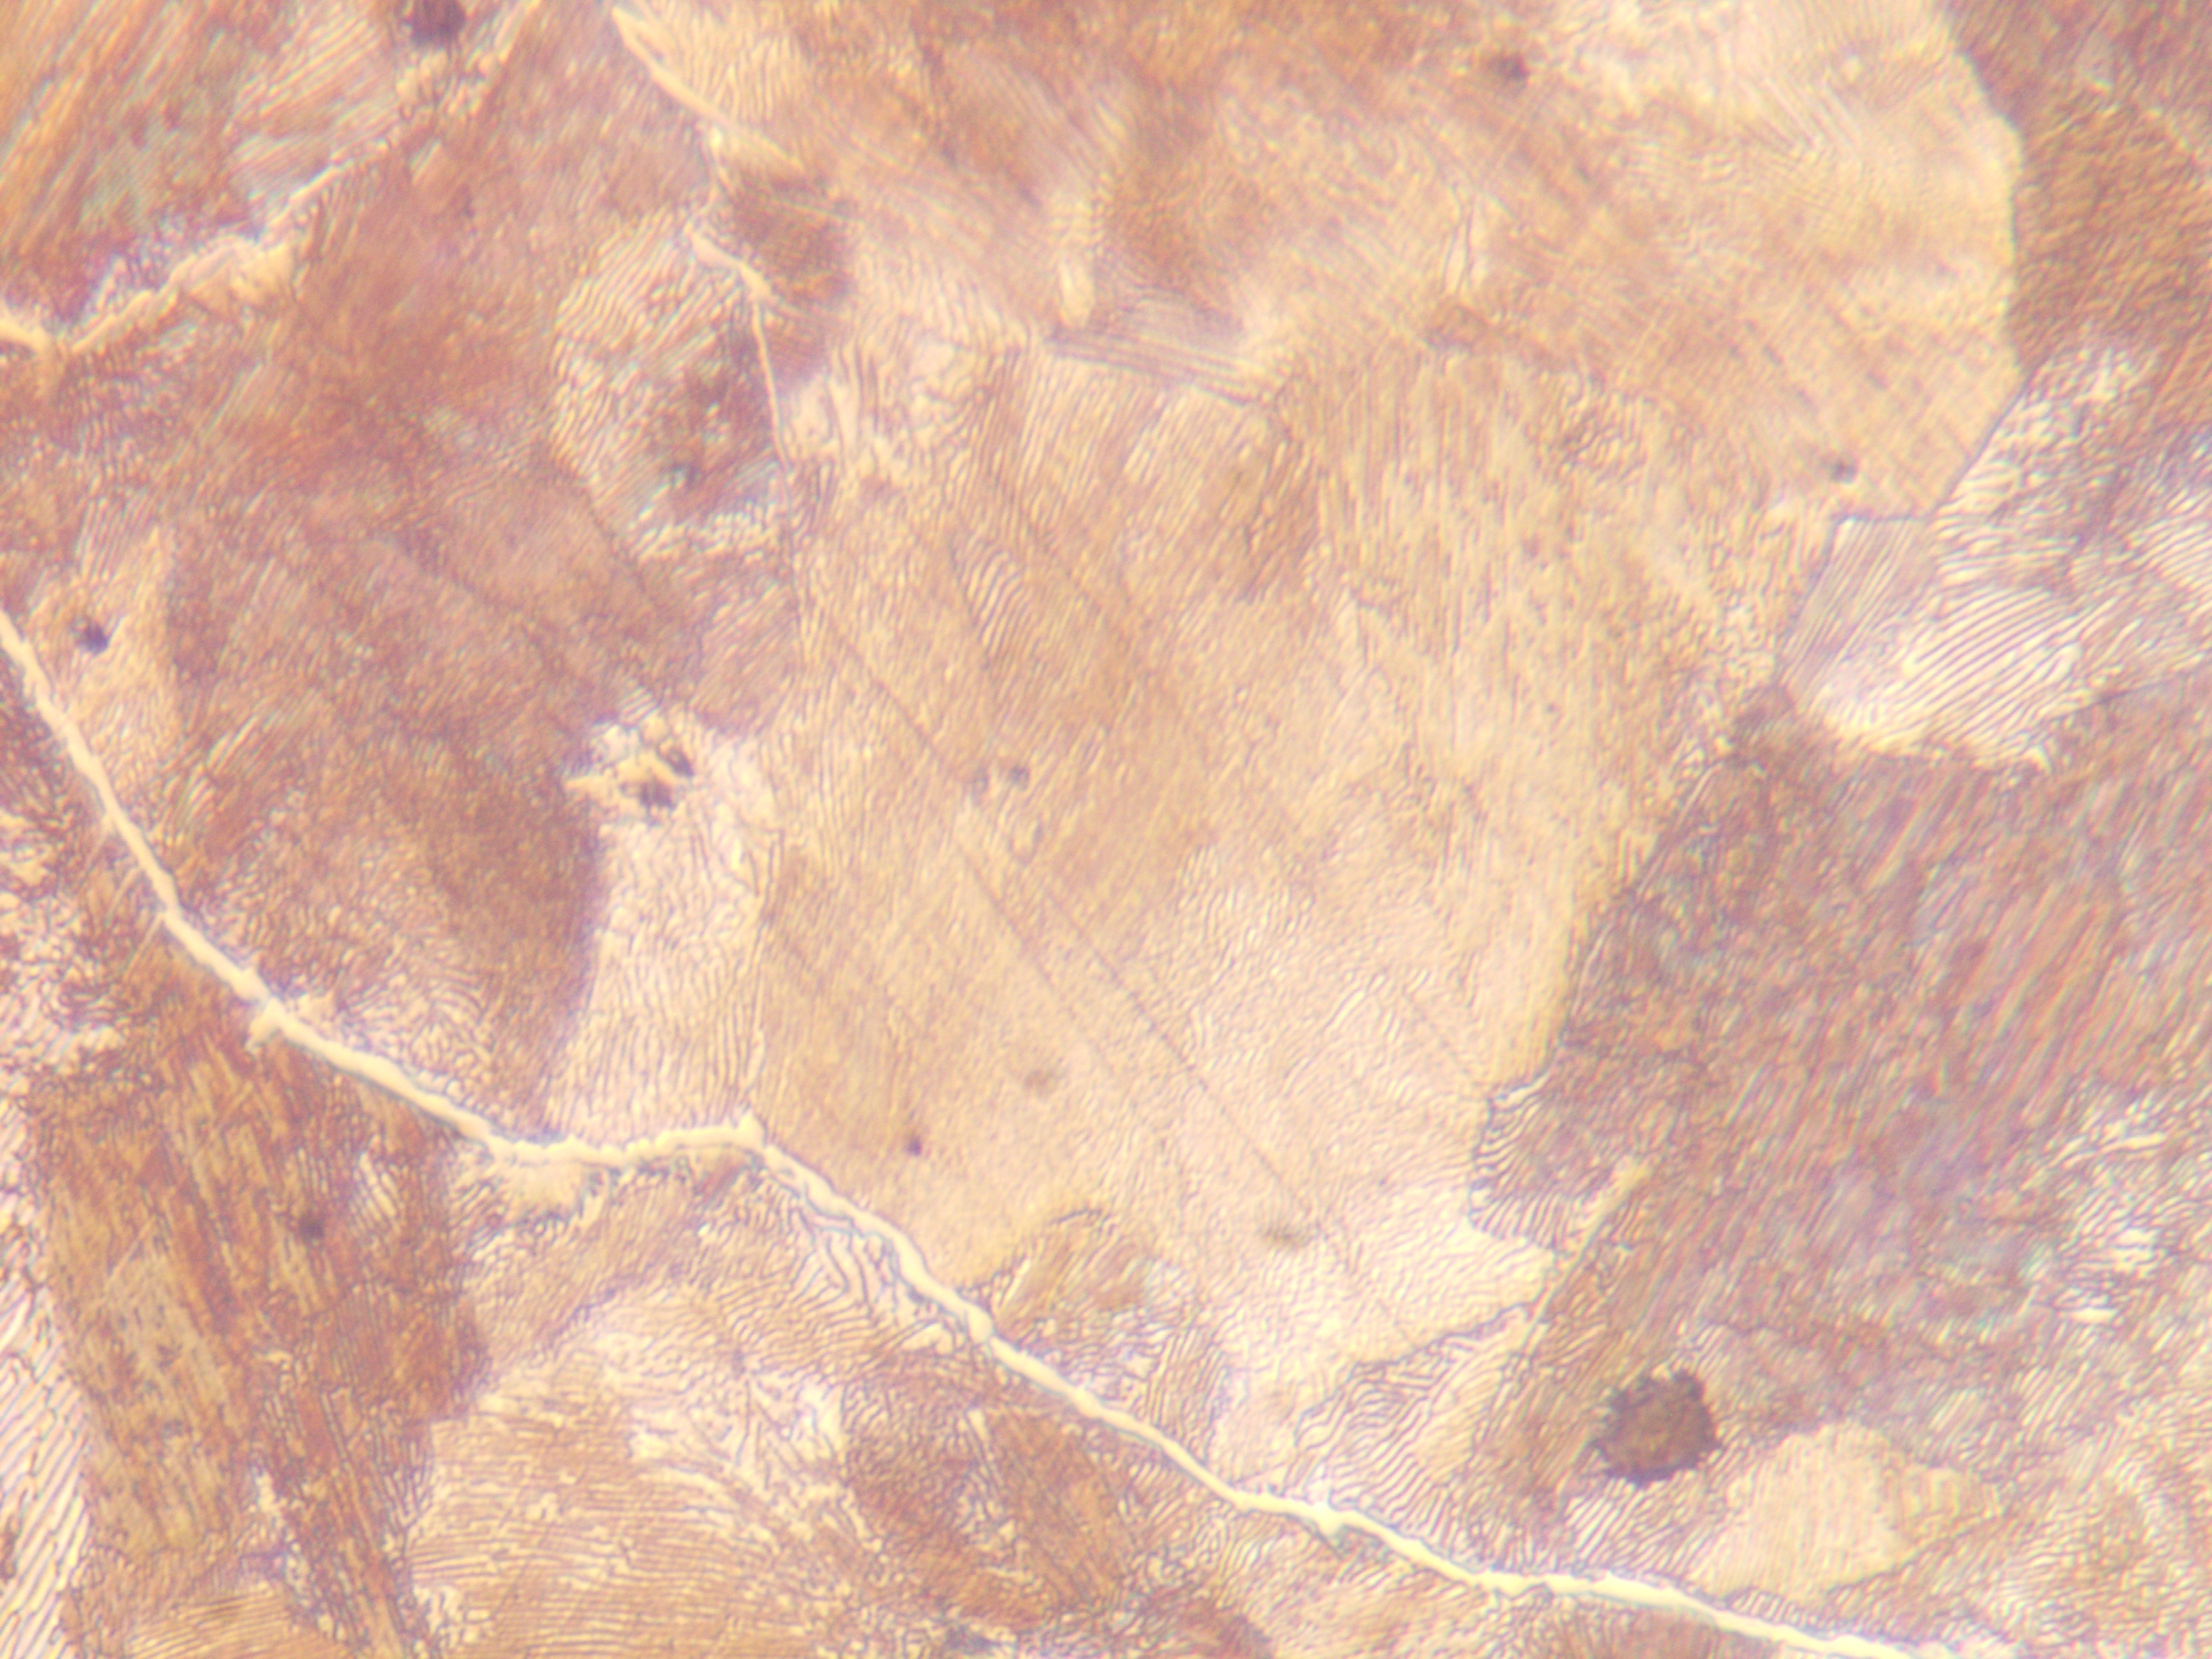
\includegraphics[width=50mm]{06-500.jpg}}
        \ffigbox[50mm]{\caption{06-T12钢}}{
\includegraphics[width=50mm]{5.png}}
    \end{floatrow}

\end{figure}

\newpage
5.亚共晶铸铁

如图九图十,亚共晶铸铁的显微组织由黑色树枝状珠光体、二次渗碳体以及片状带有部分斑点的低温莱氏体构成。
二次渗碳体在珠光体周围析出。
\begin{figure}[!ht]
    \begin{floatrow}
        \ffigbox[50mm]{\caption{08-亚共晶铸铁-200}}{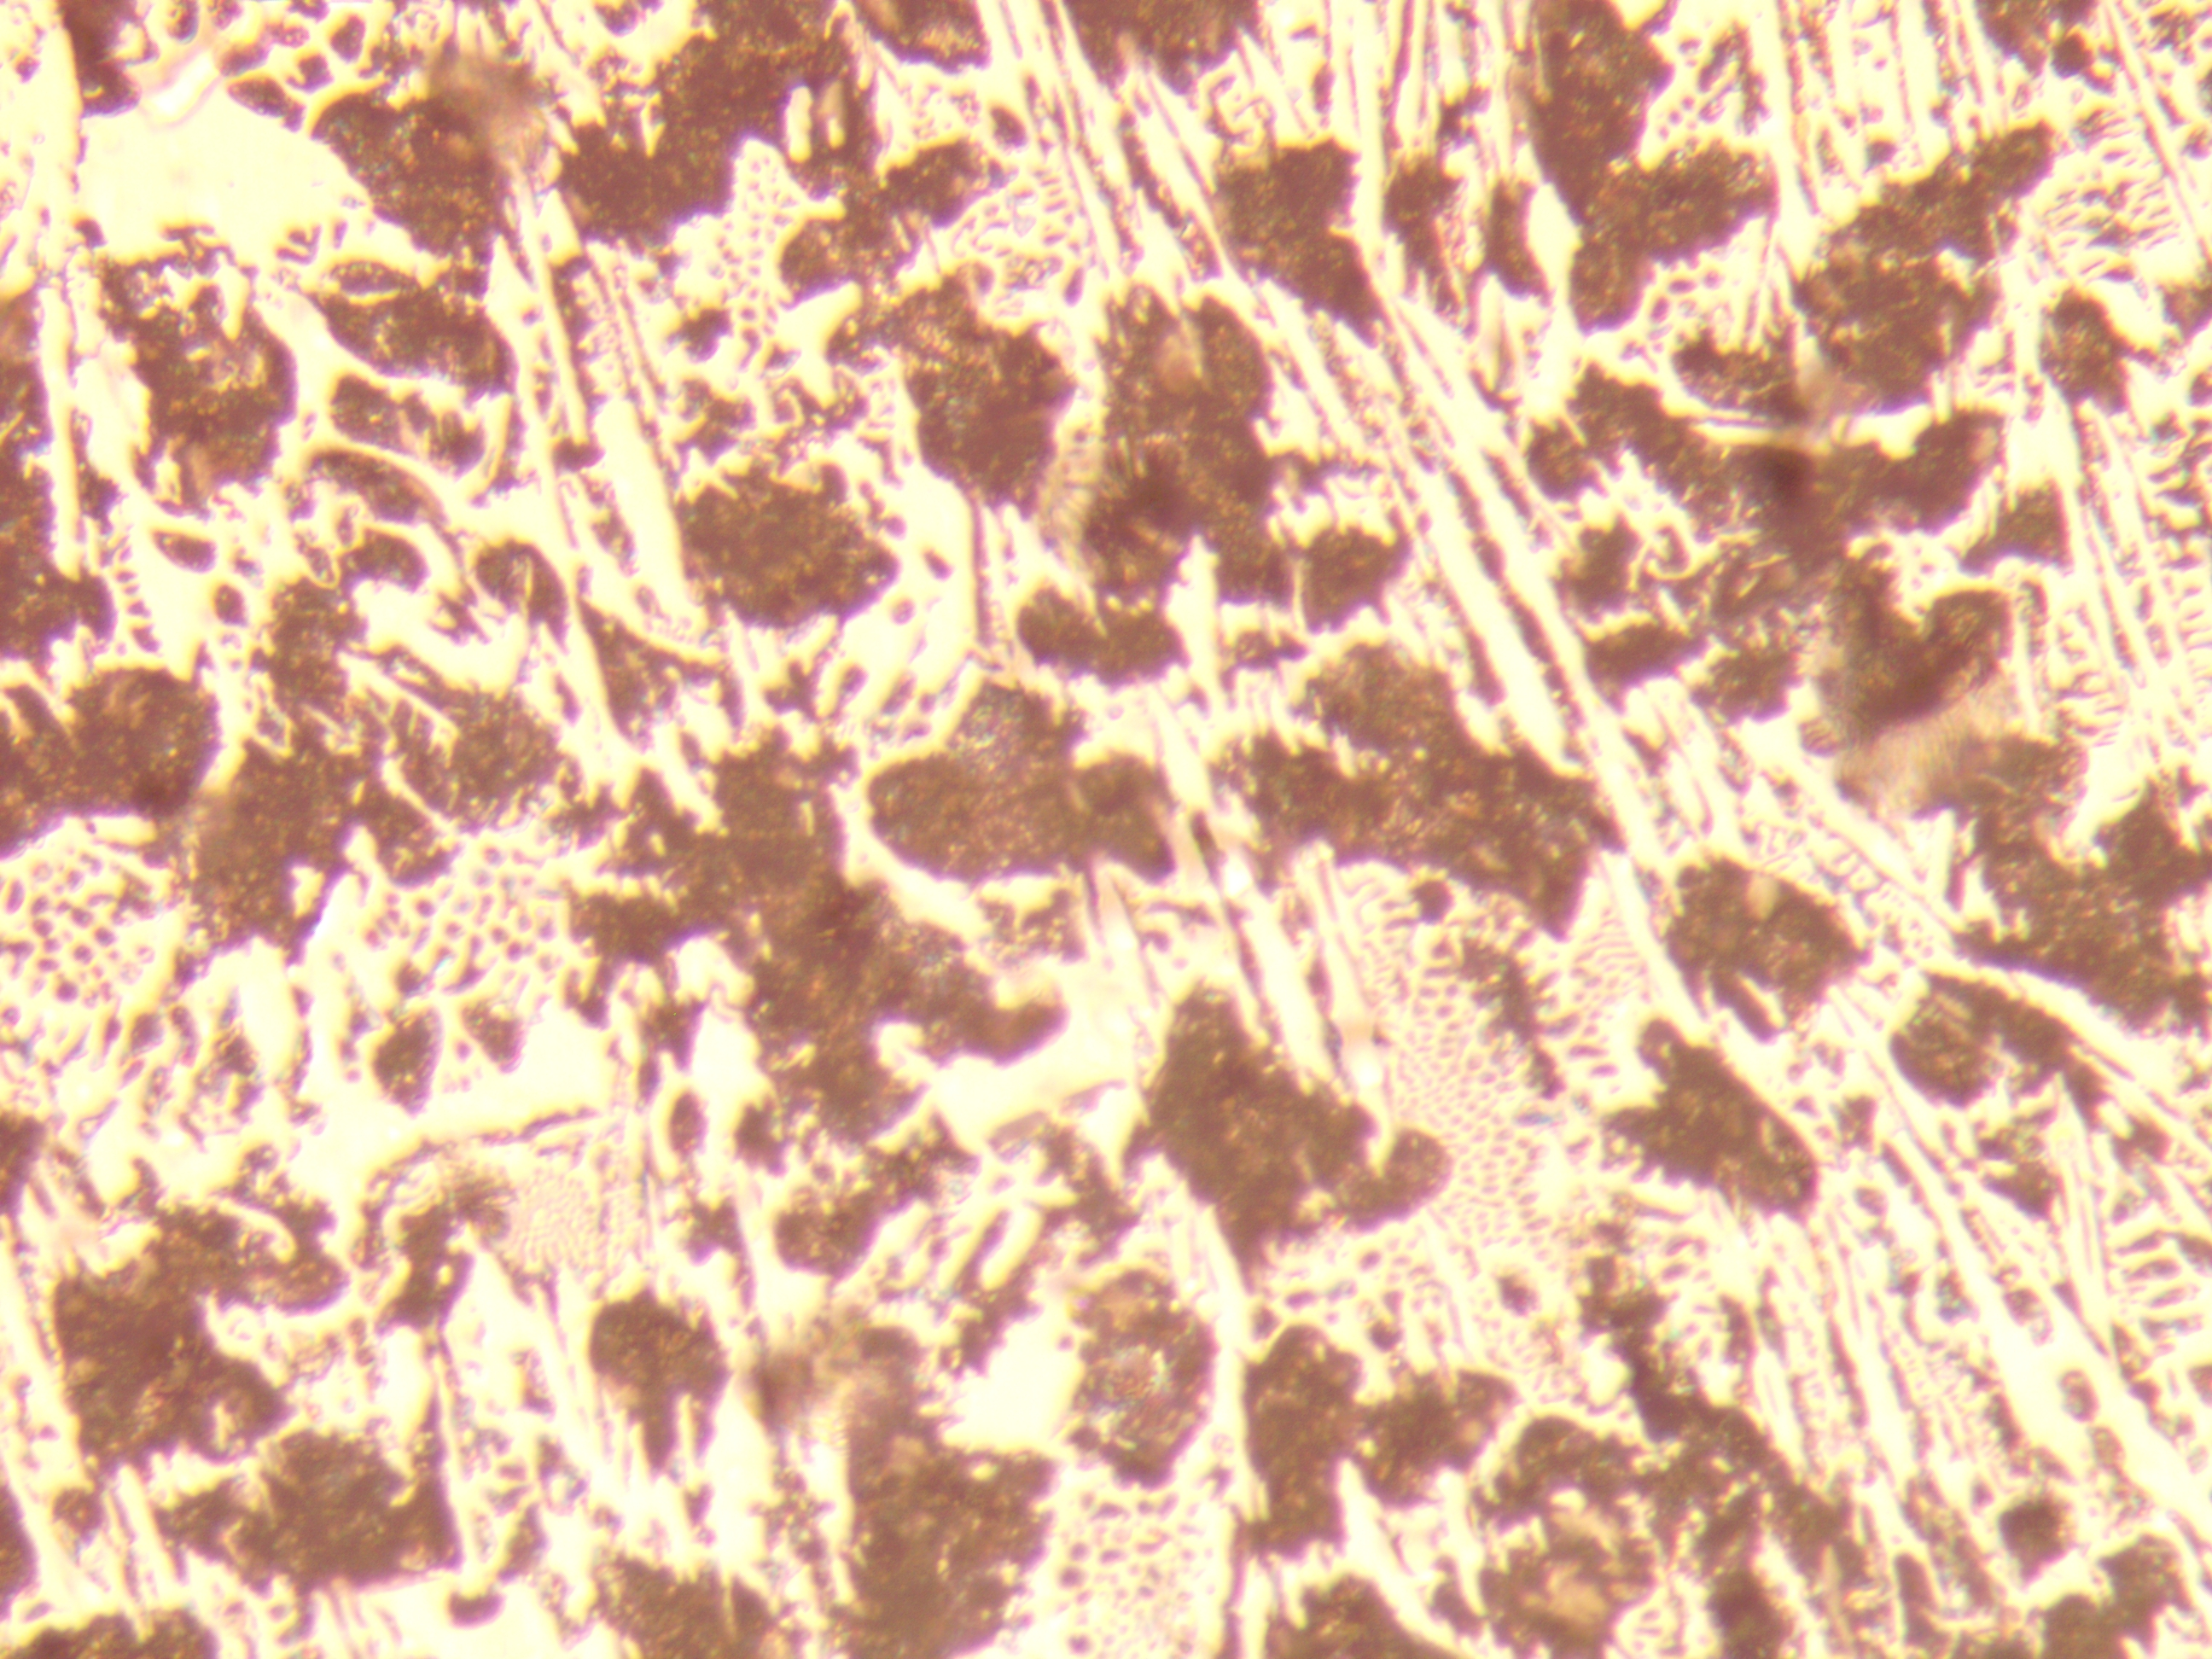
\includegraphics[width=50mm]{08-200.jpg}}
        \ffigbox[50mm]{\caption{08-亚共晶铸铁-500}}{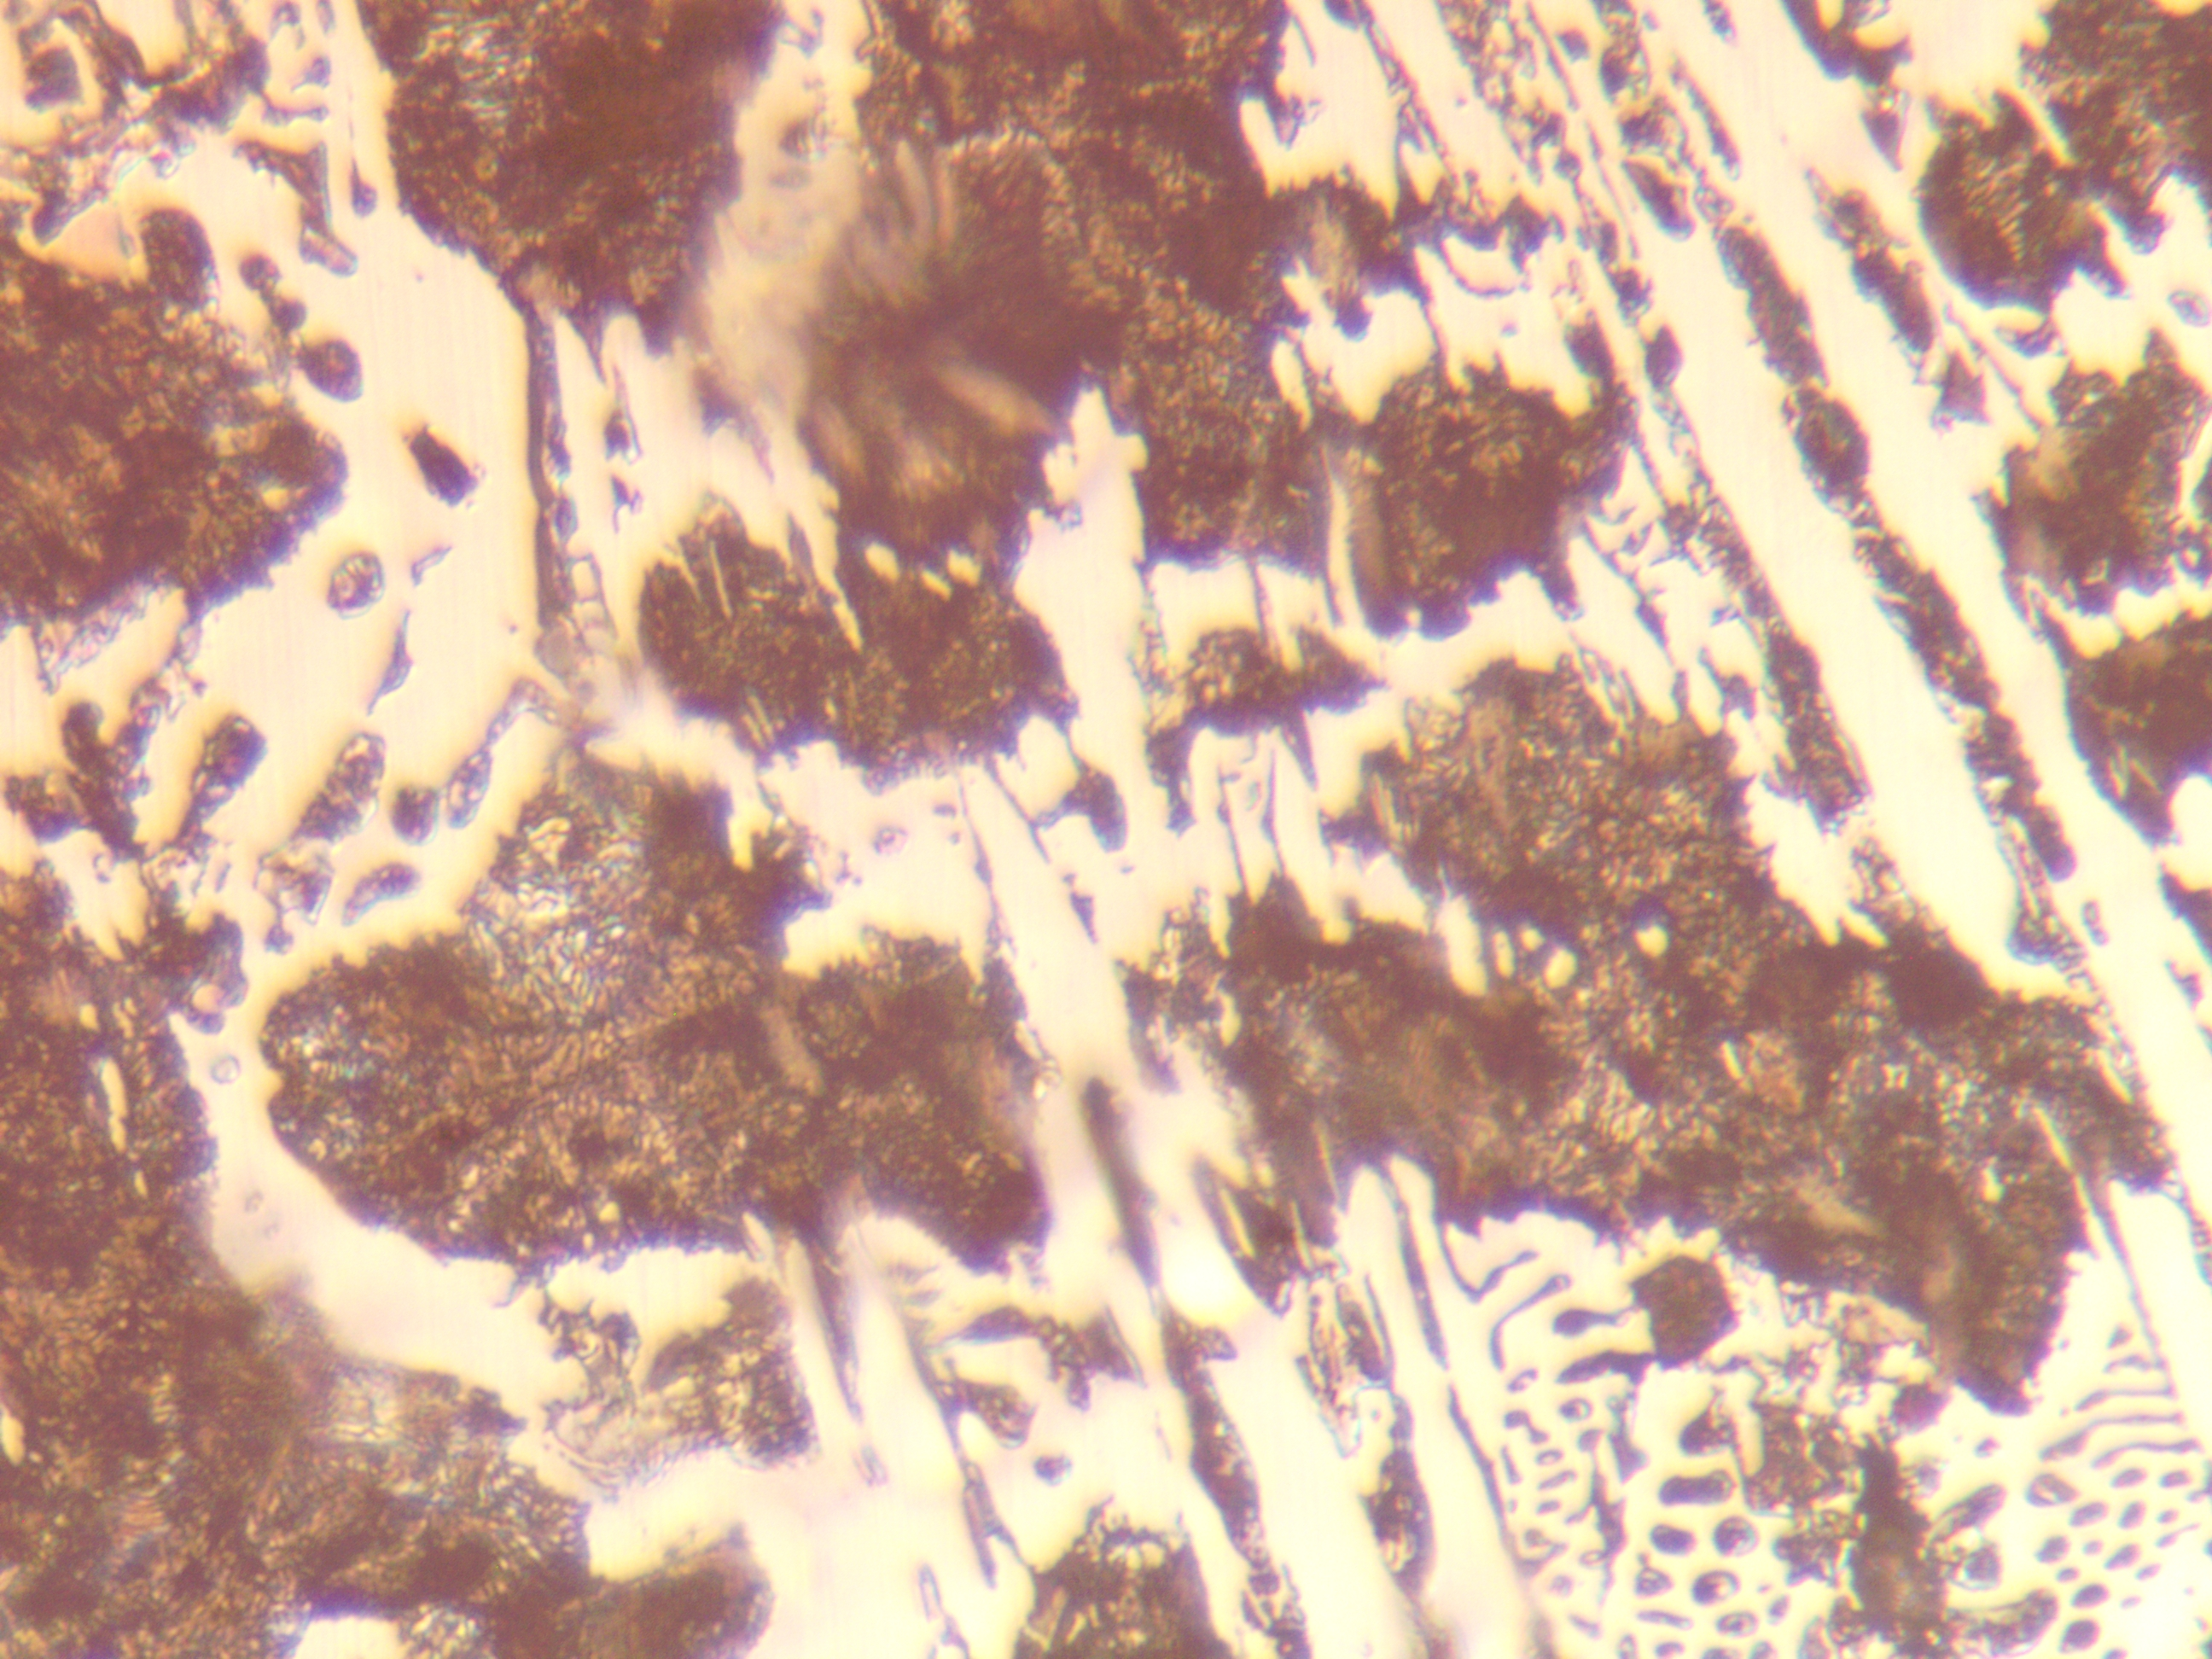
\includegraphics[width=50mm]{08-500.jpg}}
        \ffigbox[50mm]{\caption{08-亚共晶铸铁}}{
\includegraphics[width=50mm]{5.png}}
            
    \end{floatrow}

\end{figure}

6.共晶铸铁

如,图十一,十二,显微镜下呈现共晶低温莱氏体的纹路状结构,有点状的低温莱氏体镶嵌在中间,
白色基体为共晶渗碳体,珠光体应该为片层状,同时珠光体因无法分辨而呈现黑色。
\begin{figure}[!ht]
    \begin{floatrow}
        \ffigbox[50mm]{\caption{09-共晶铸铁-200}}{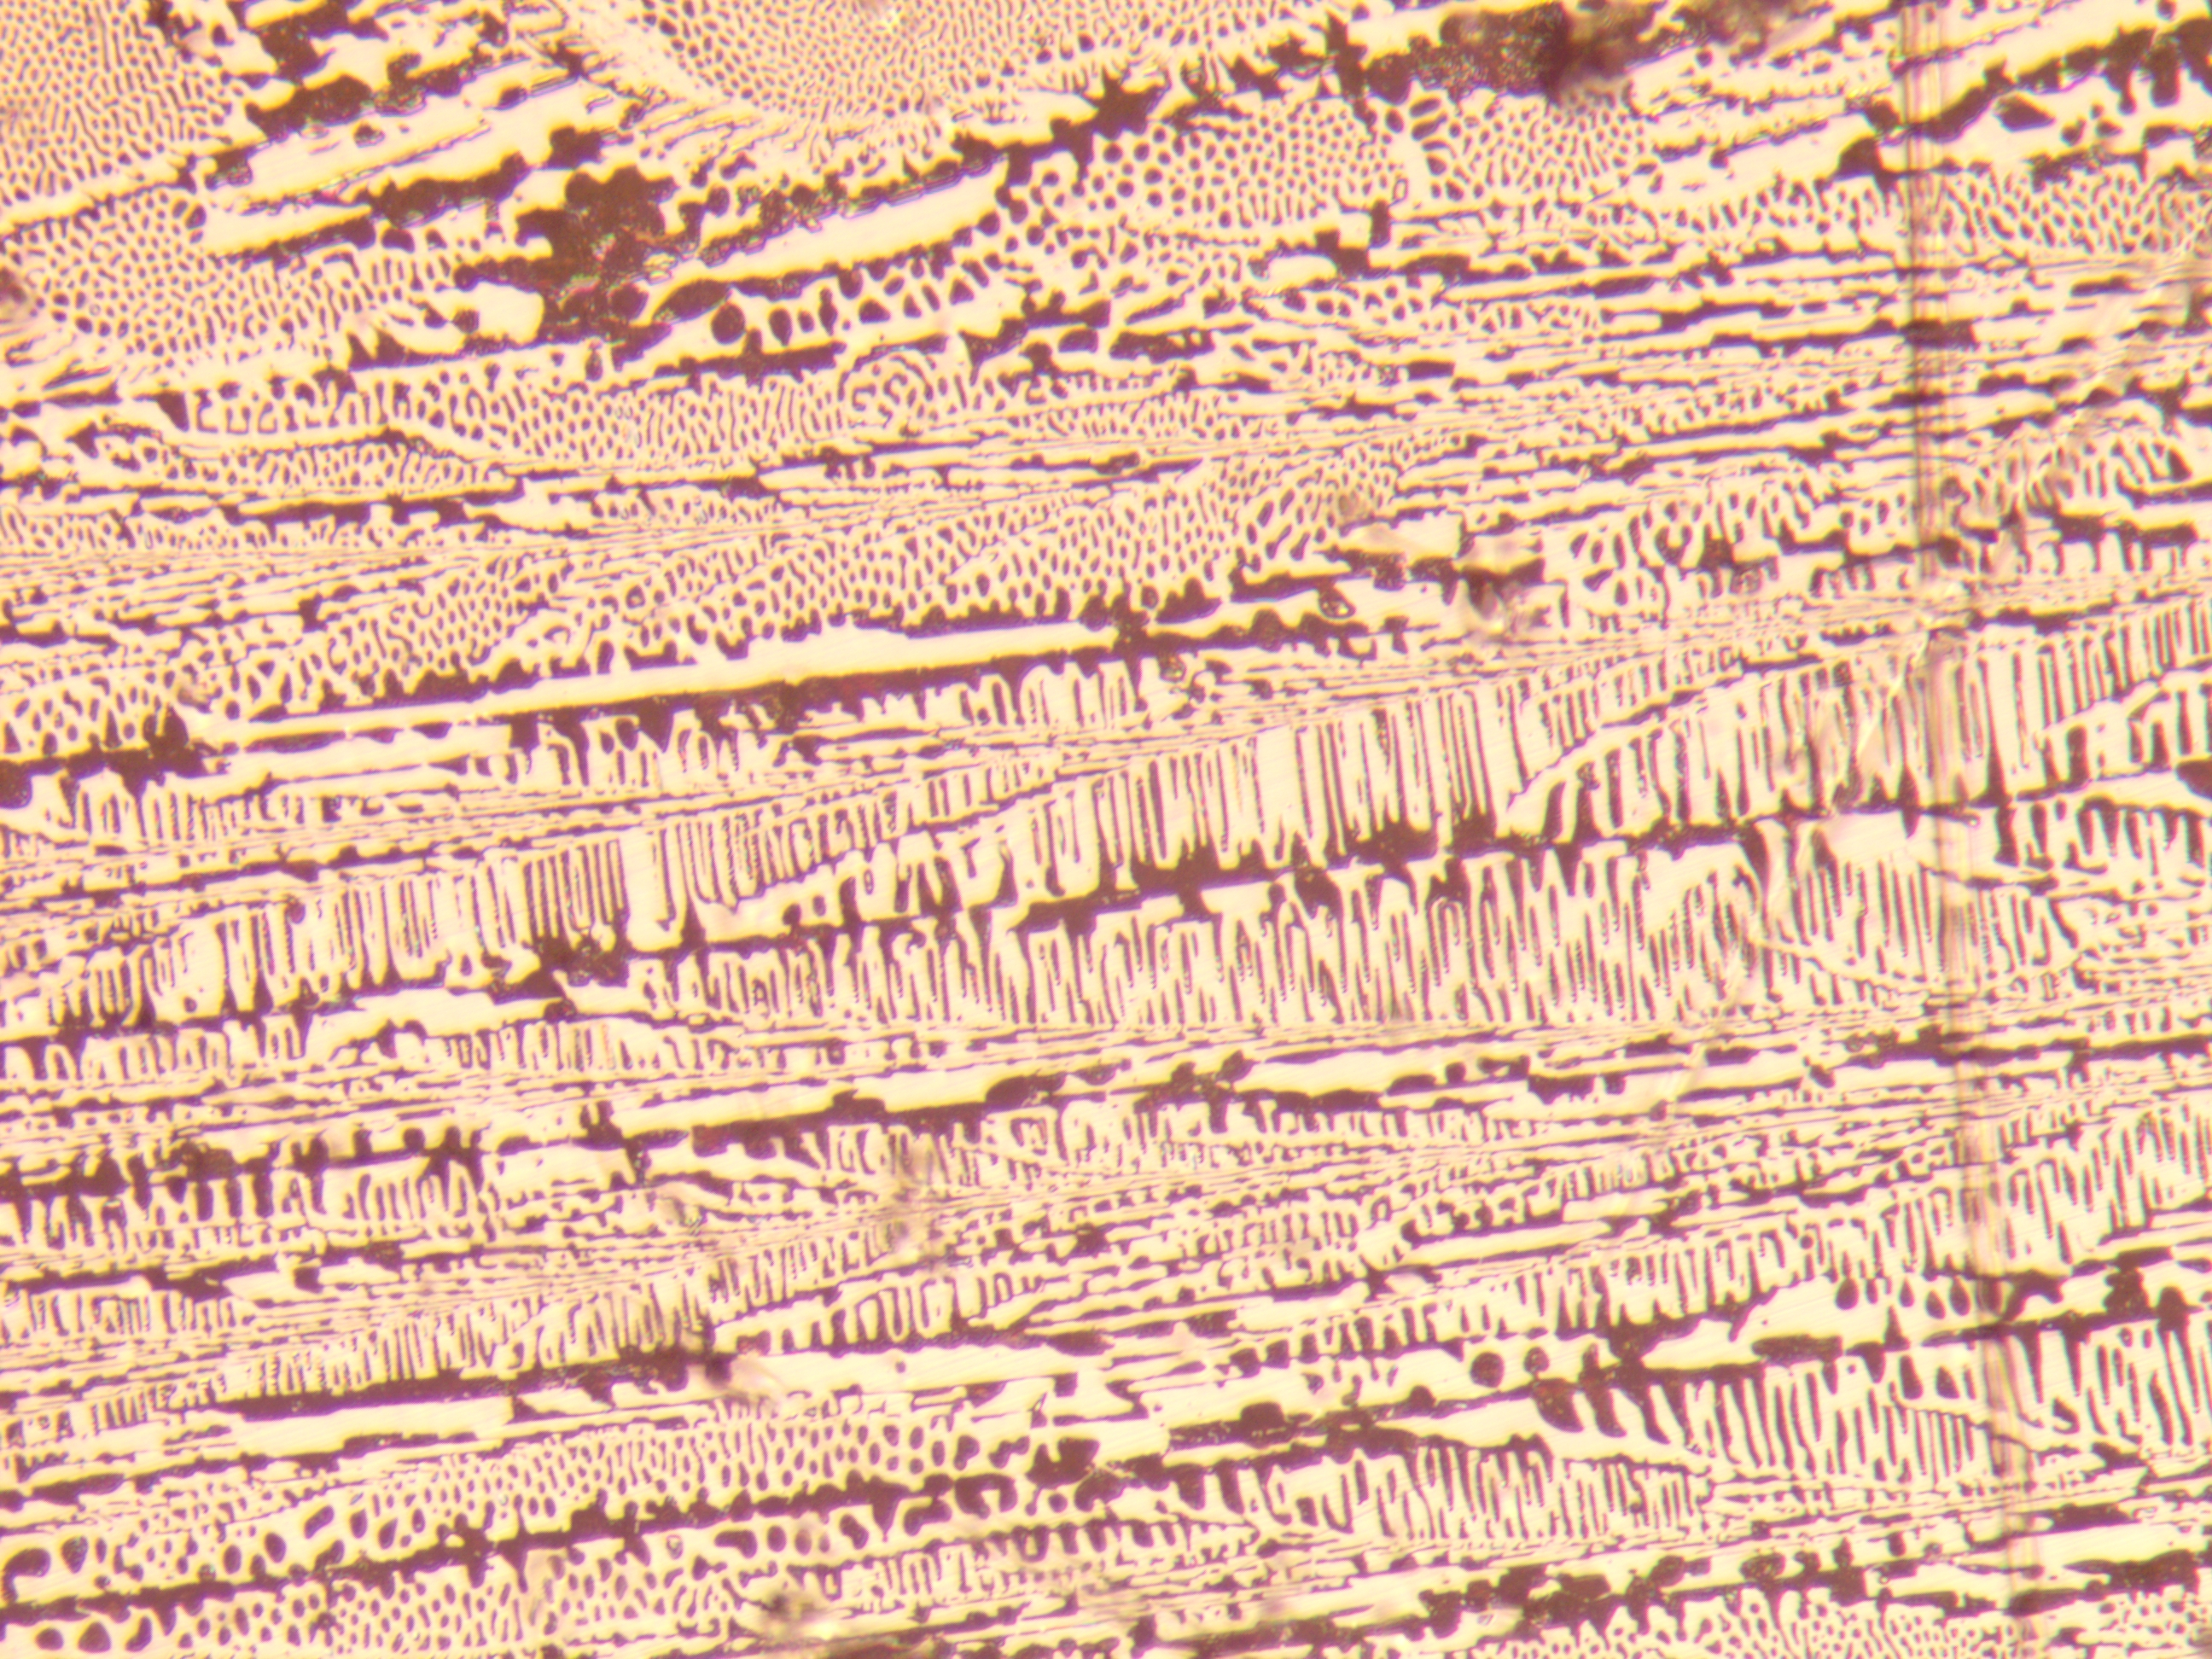
\includegraphics[width=50mm]{09-200.jpg}}
        \ffigbox[50mm]{\caption{09-共晶铸铁-200}}{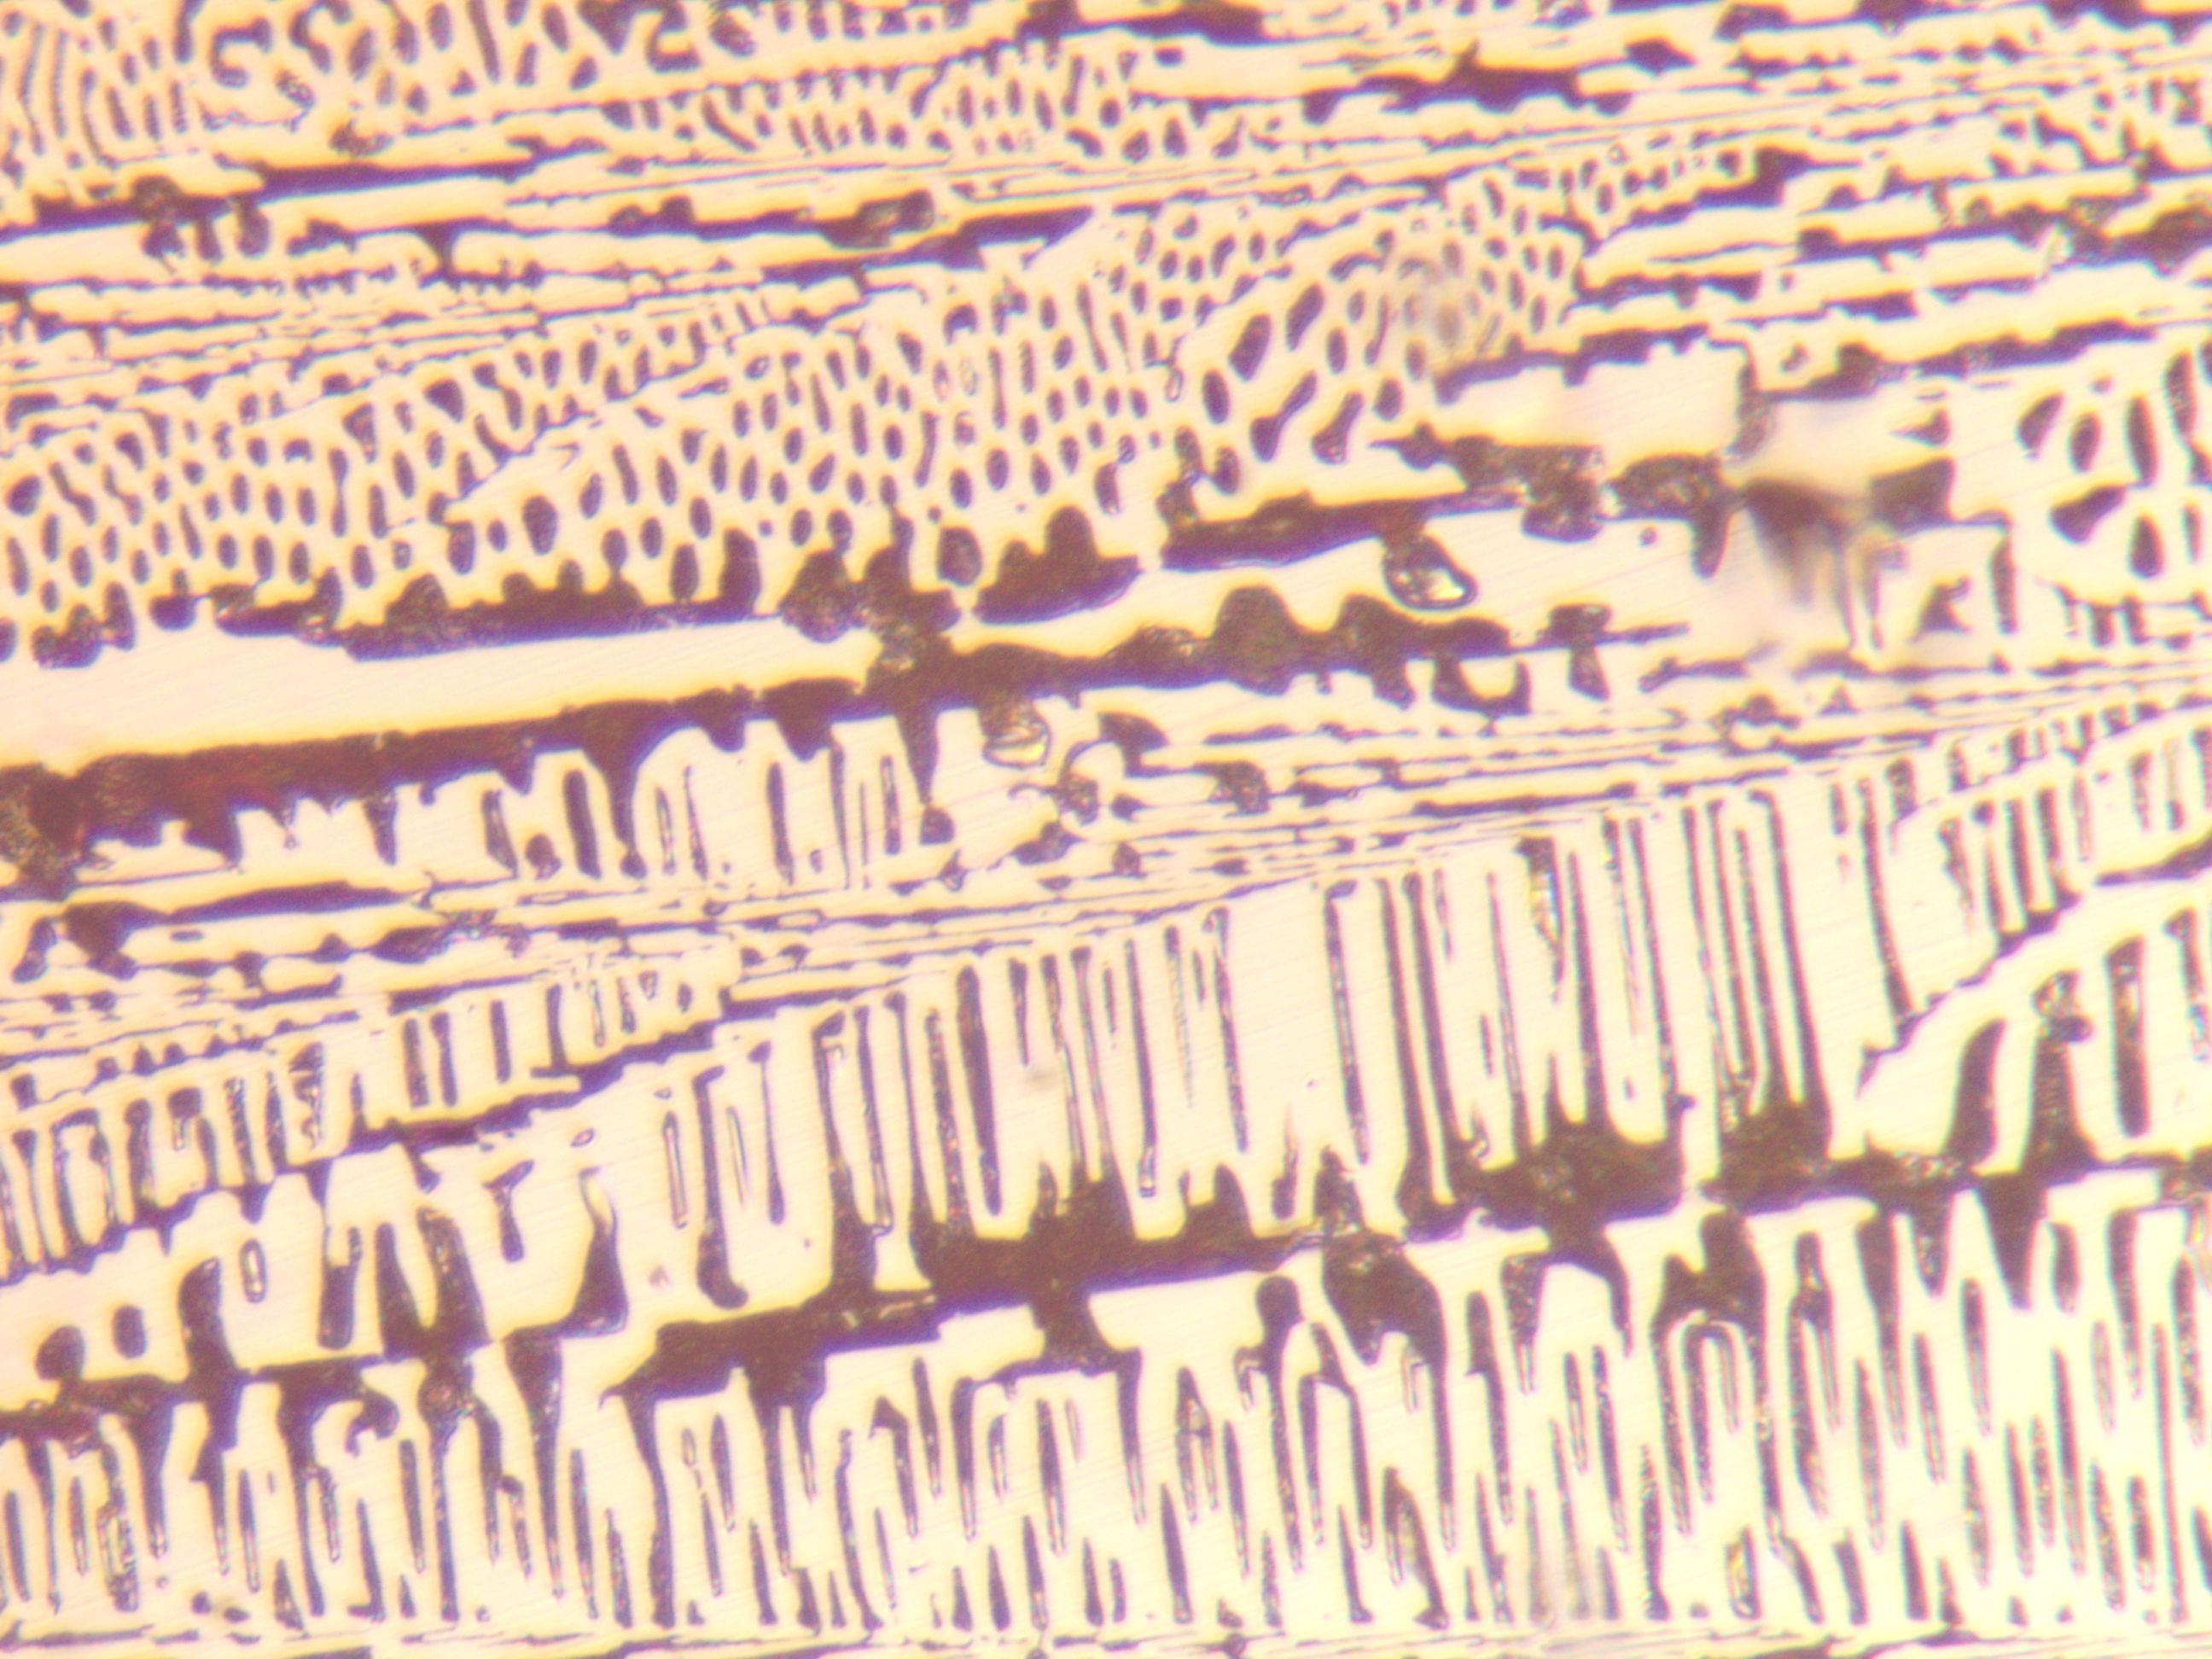
\includegraphics[width=50mm]{09-500.jpg}}
        \ffigbox[50mm]{\caption{09-共晶铸铁}}{
\includegraphics[width=50mm]{5.png}}
            
    \end{floatrow}

\end{figure}

\newpage
7.过共晶铸铁

如图十三,图十四,白亮色部分为一次渗碳体,呈现板条状,中间夹杂的共晶莱氏体。共晶莱氏体的微观结构
由点状的部分和更深颜色的连续部分组成。
\begin{figure}[!ht]
    \begin{floatrow}
        \ffigbox[50mm]{\caption{10-过共晶铸铁-200}}{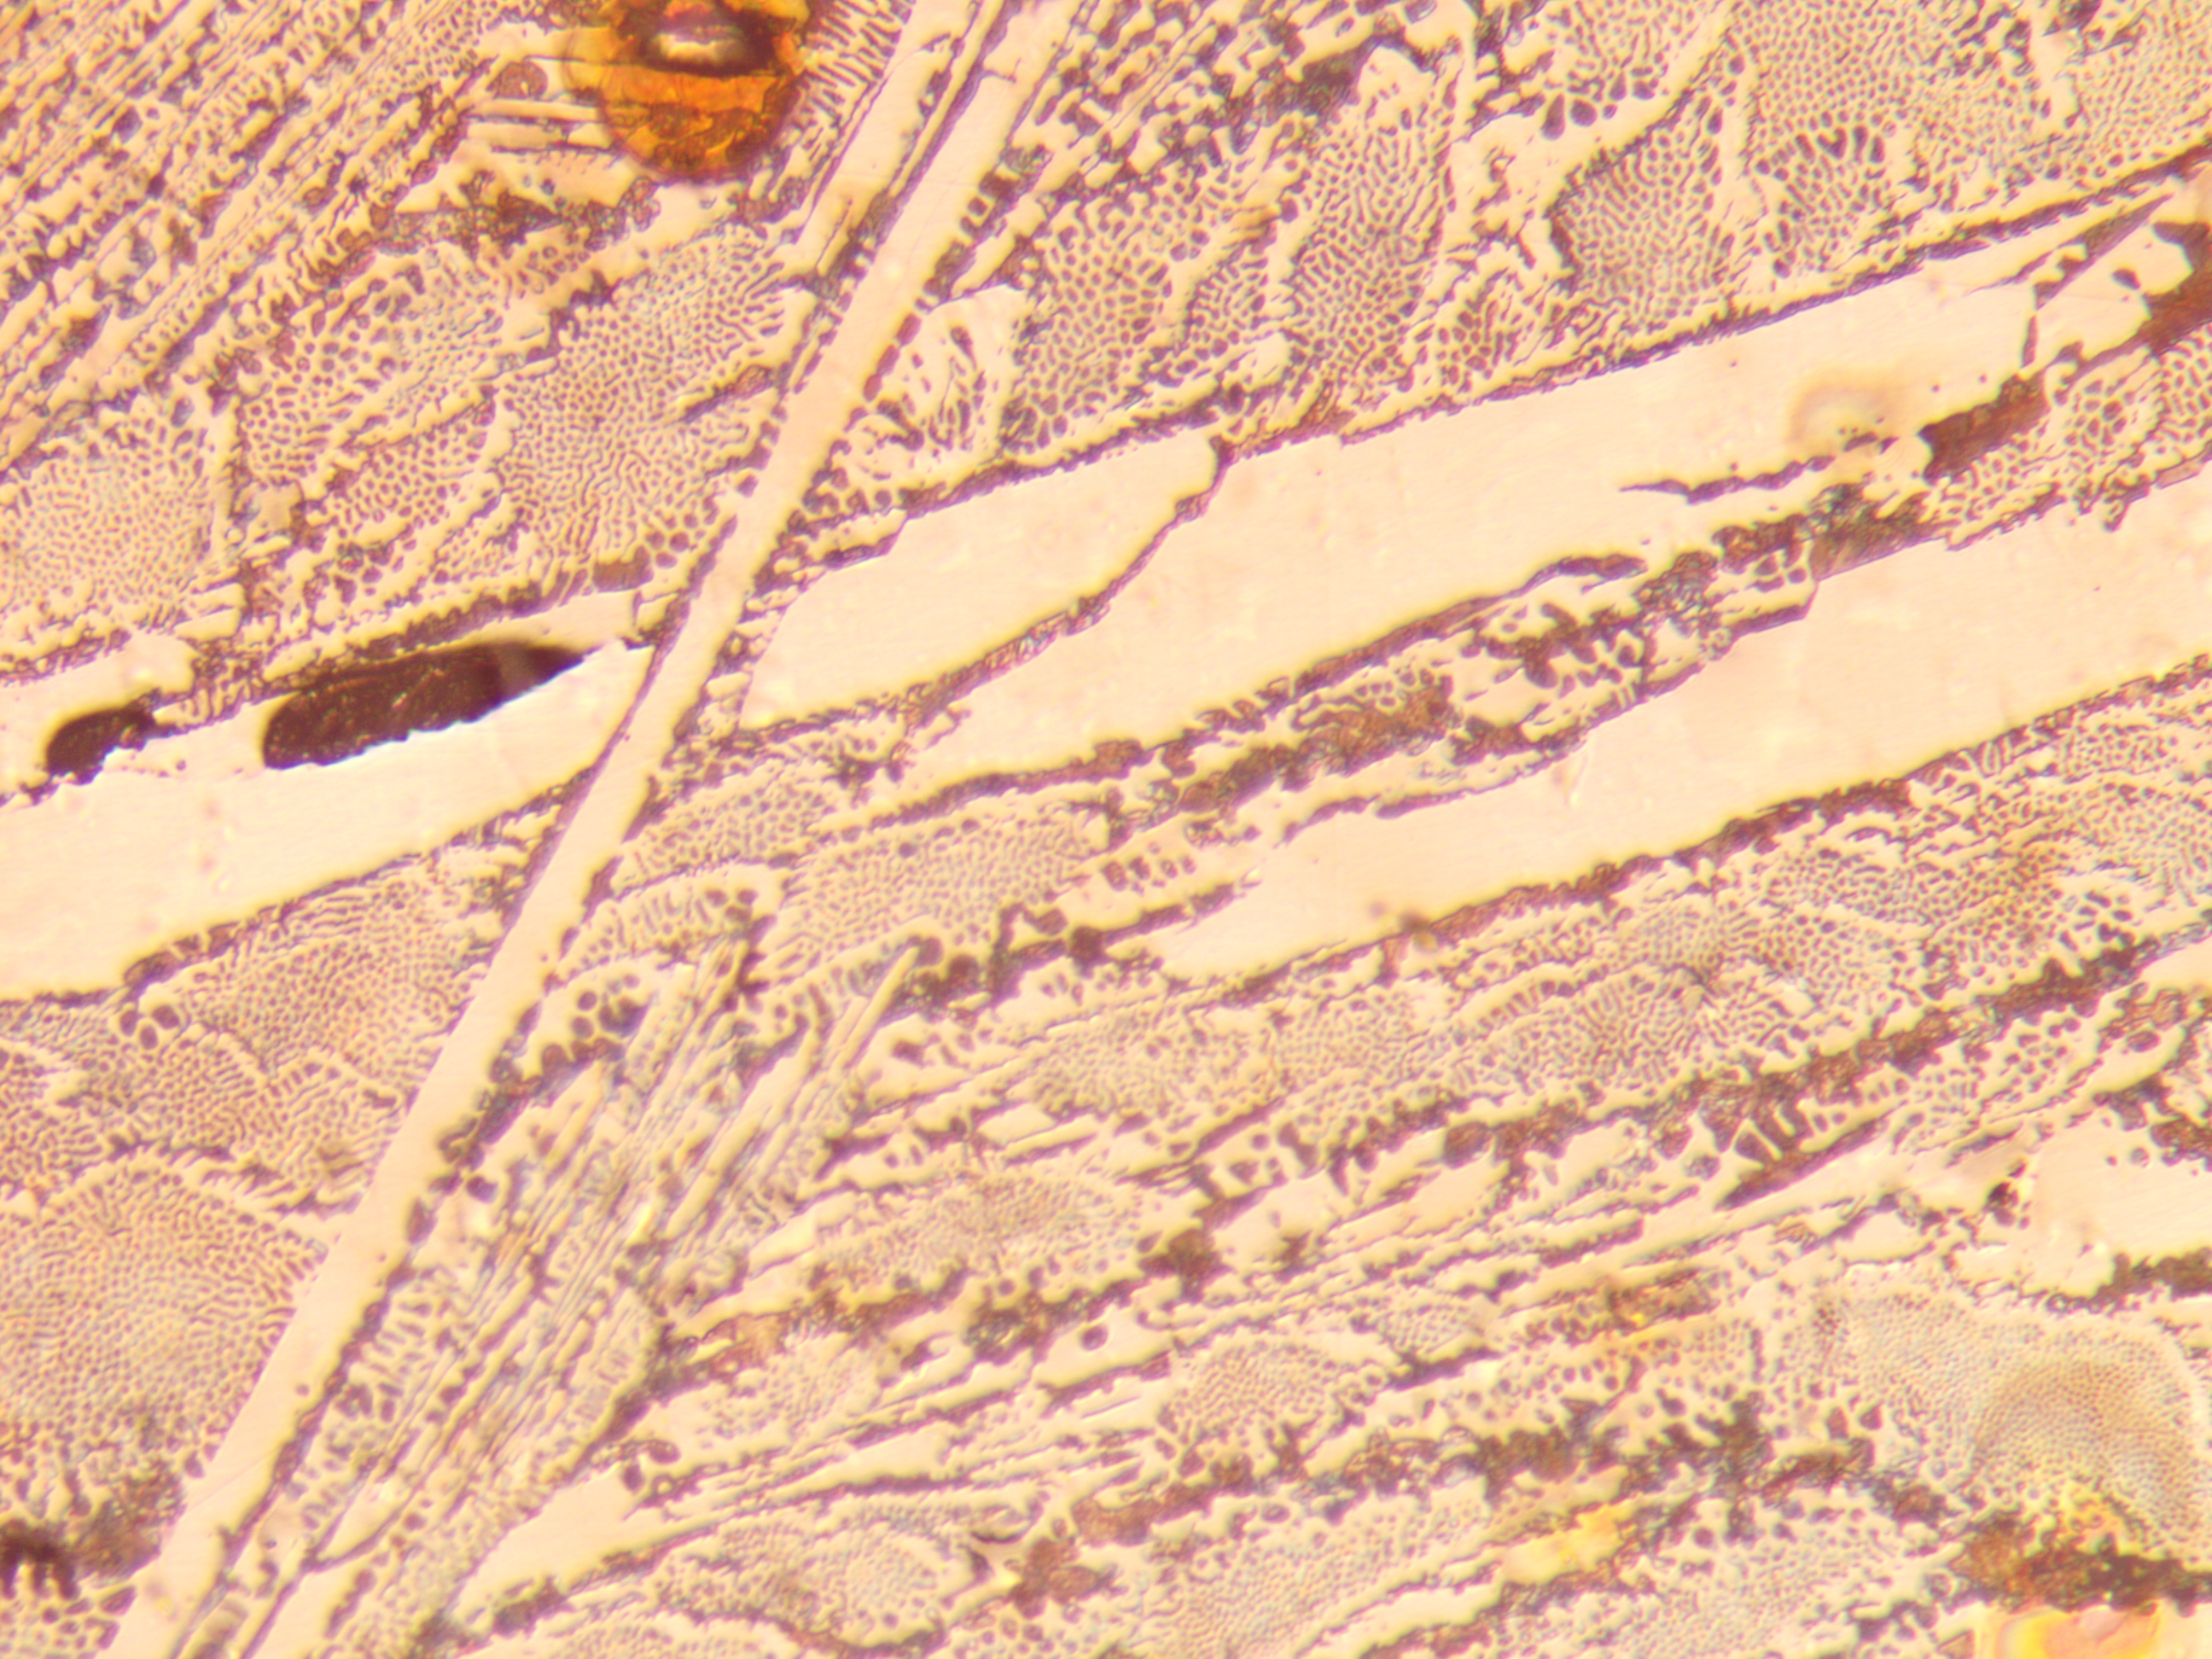
\includegraphics[width=50mm]{10-200.jpg}}
        \ffigbox[50mm]{\caption{10-过共晶铸铁-500}}{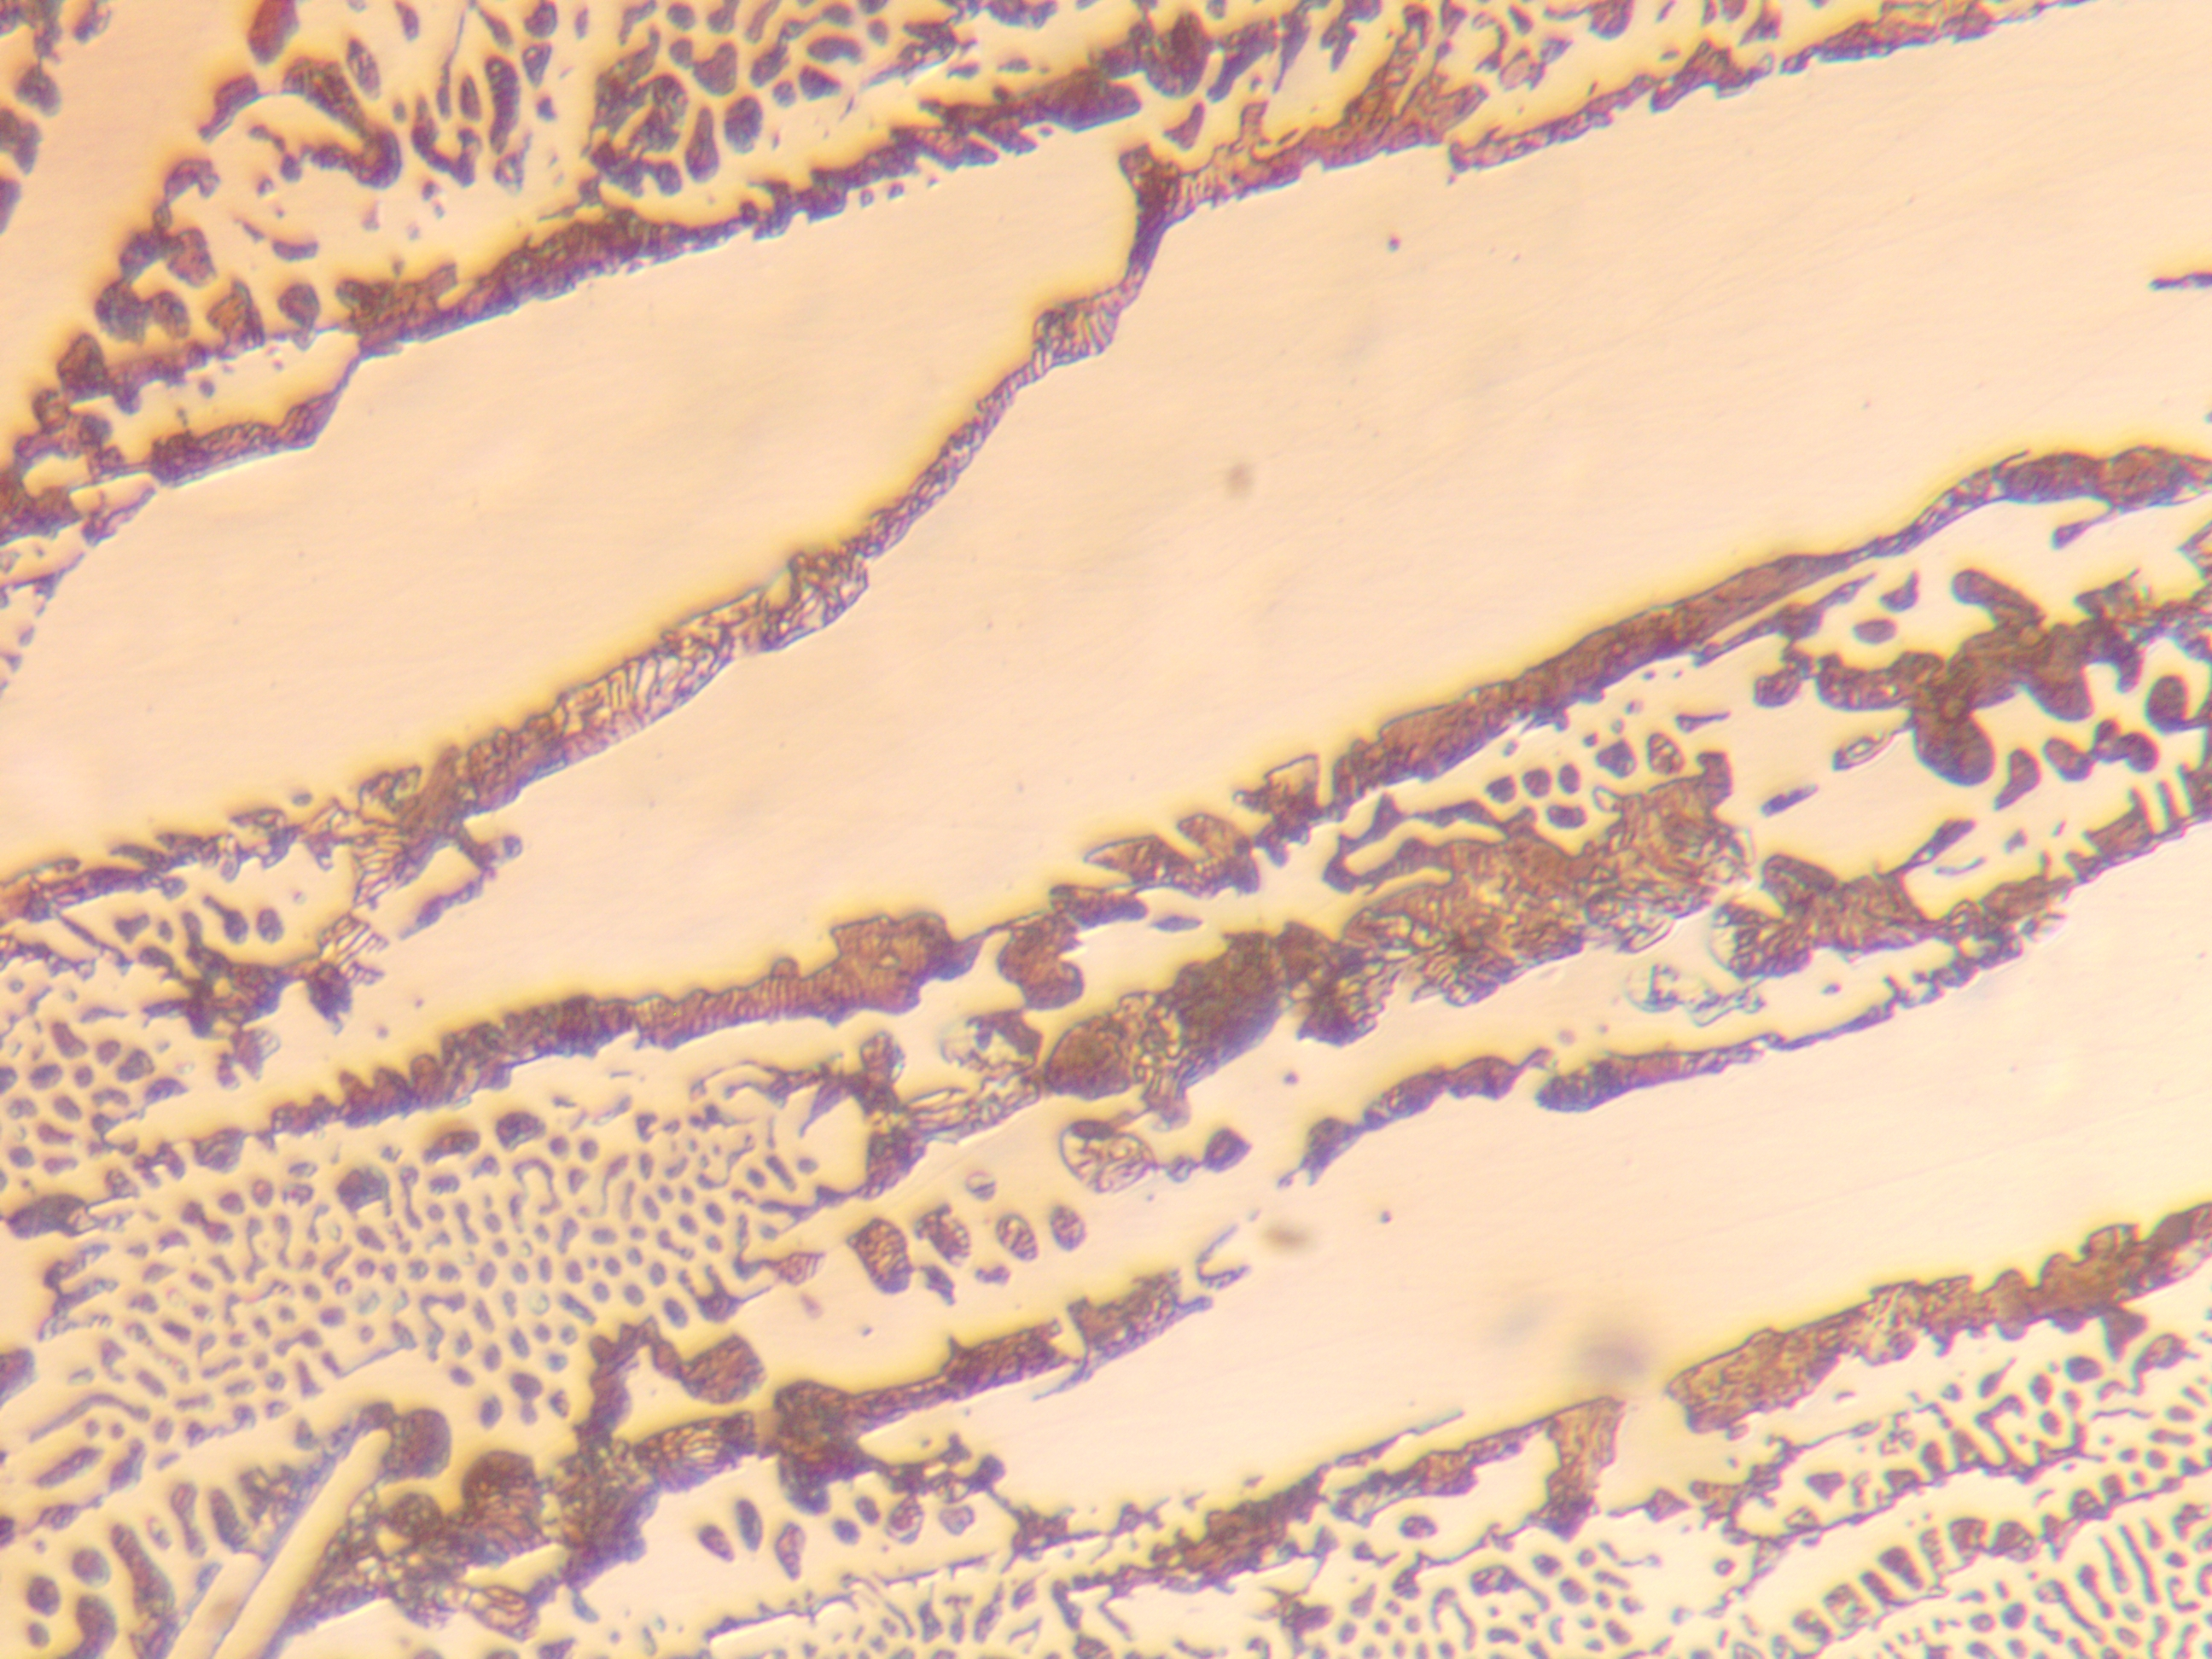
\includegraphics[width=50mm]{10-500.jpg}}
        \ffigbox[50mm]{\caption{10-过共晶铸铁}}{
\includegraphics[width=50mm]{5.png}}
            
    \end{floatrow}

\end{figure}

8.\#21,45钢860°C水淬+中温回火

如图十五,图十六,显微组织下的结构呈现回火屈氏体的特征,马氏体针状形态消失,但仍隐约可见;
铁素体基体上分布有细粒状渗碳体。
\begin{figure}[!ht]
    \begin{floatrow}
        \ffigbox[50mm]{\caption{21-200}}{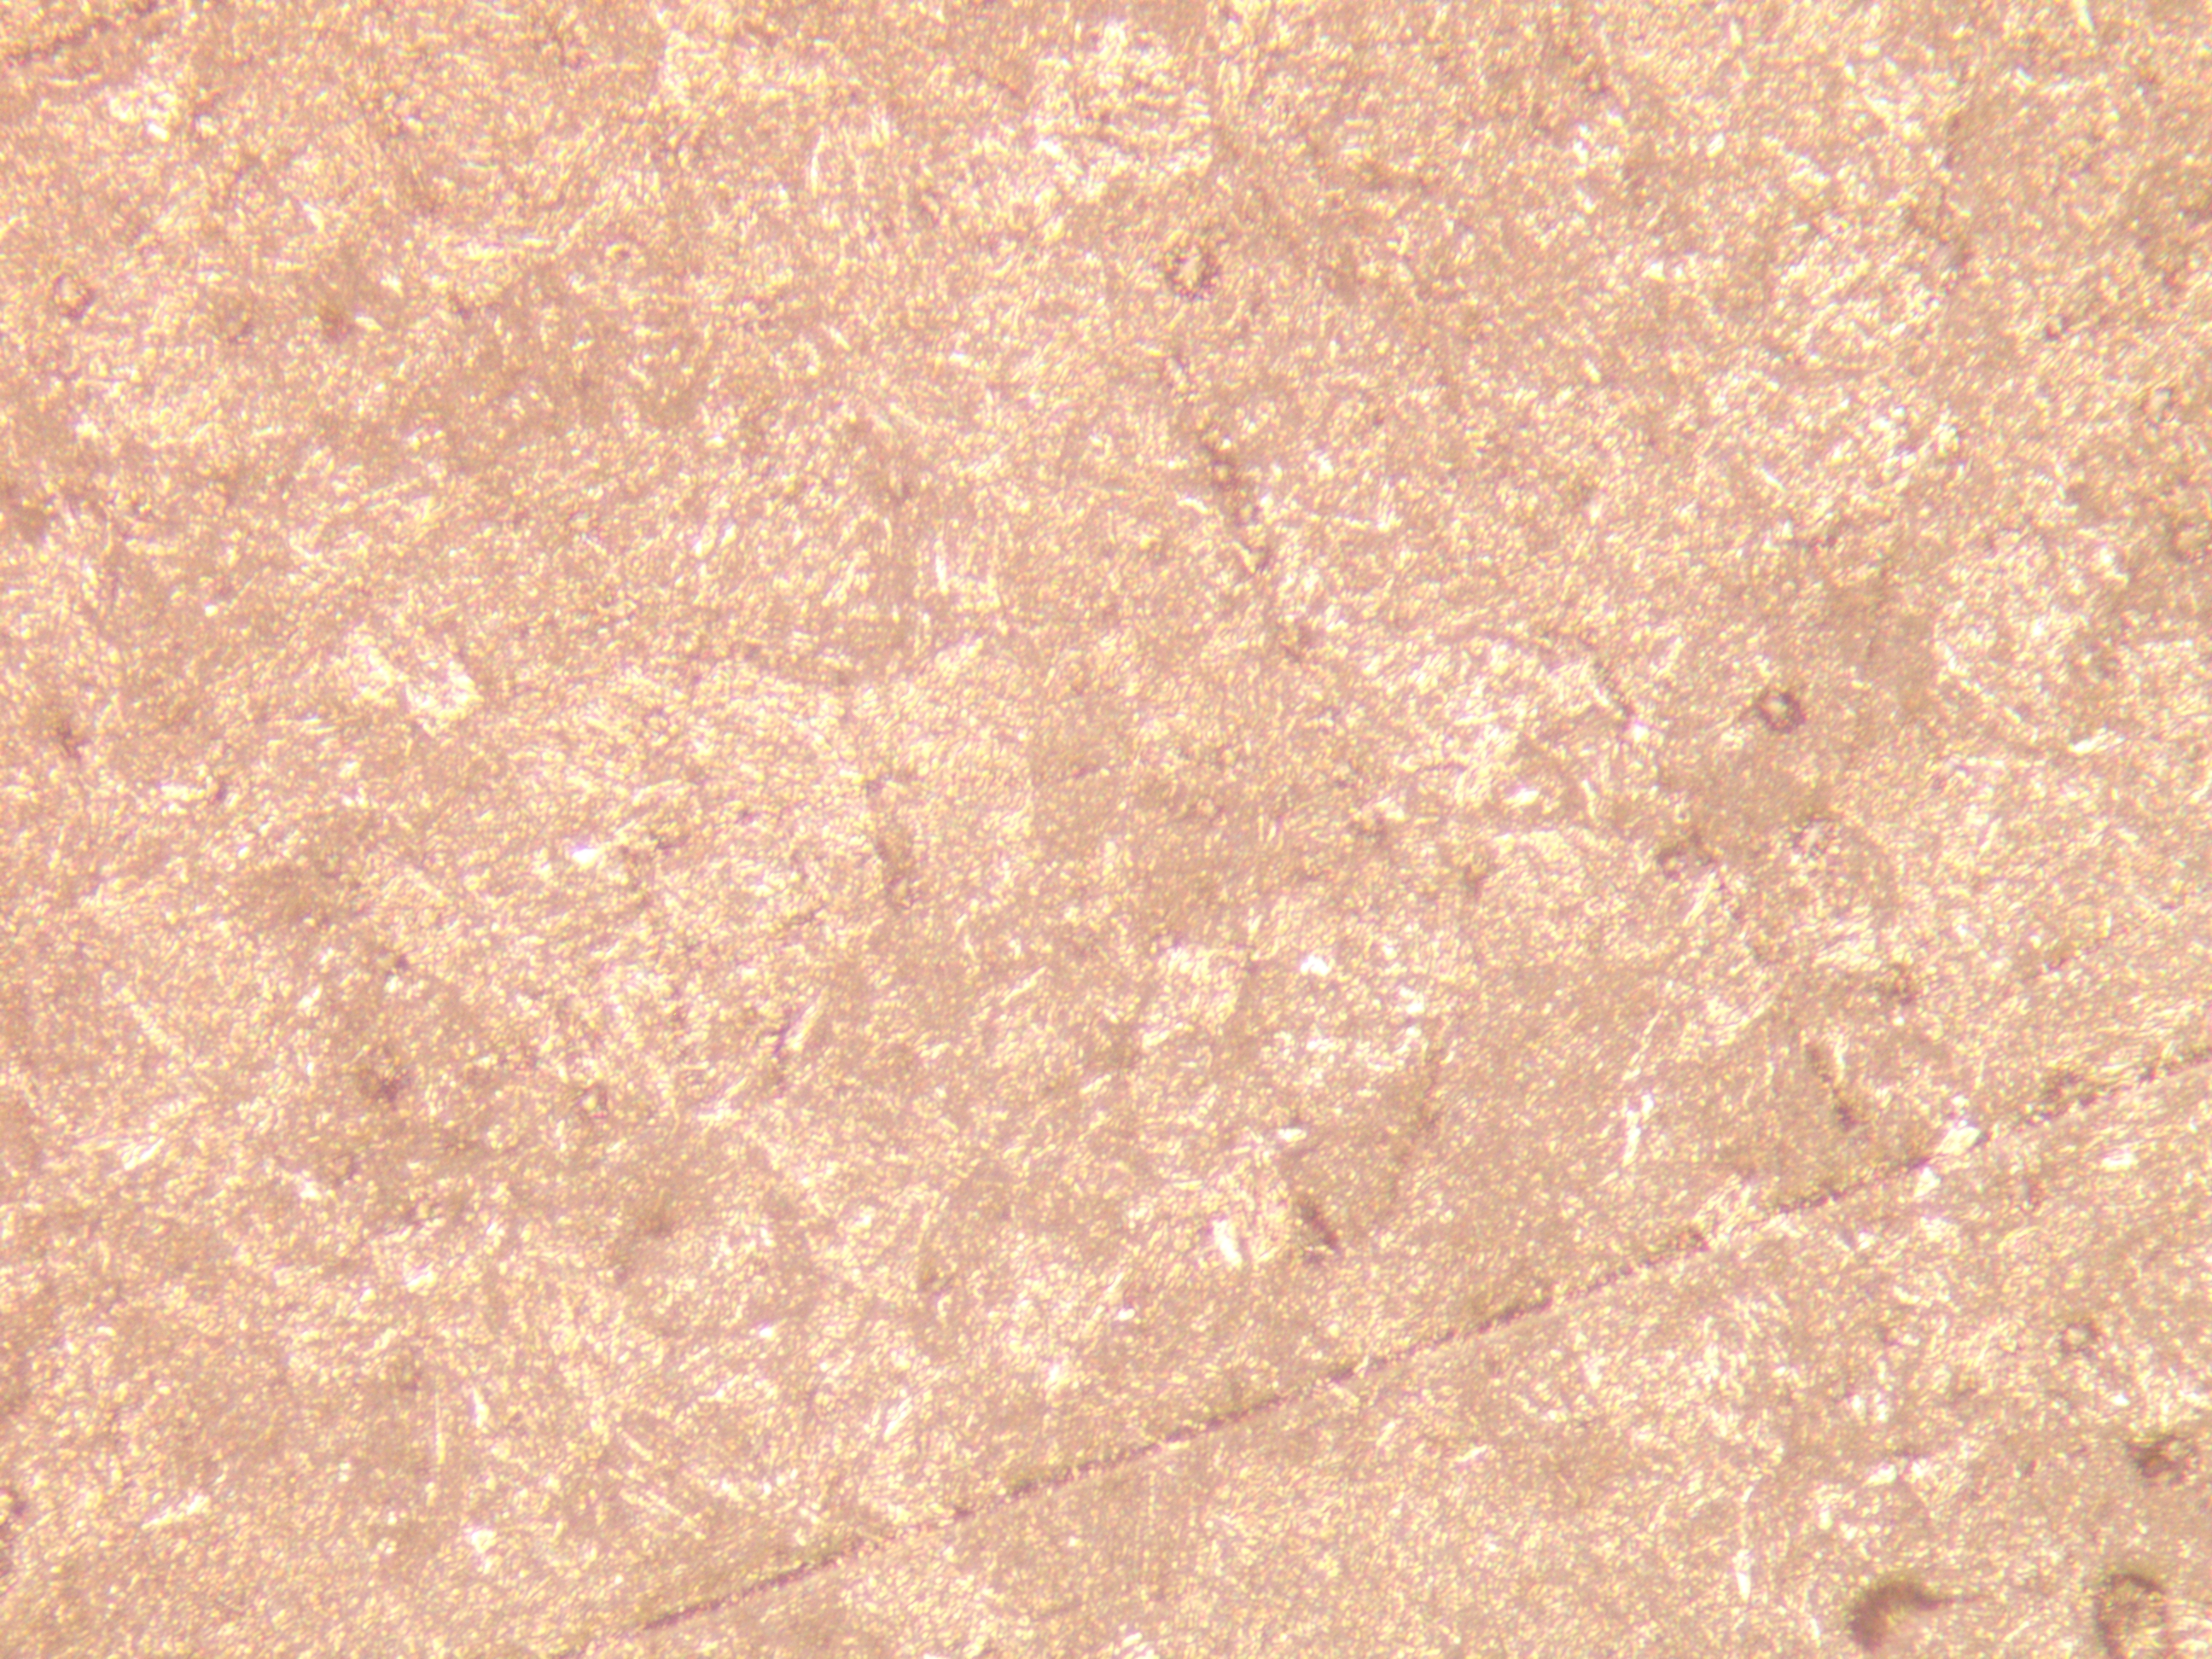
\includegraphics[width=50mm]{21-200.jpg}}
        \ffigbox[50mm]{\caption{21-500}}{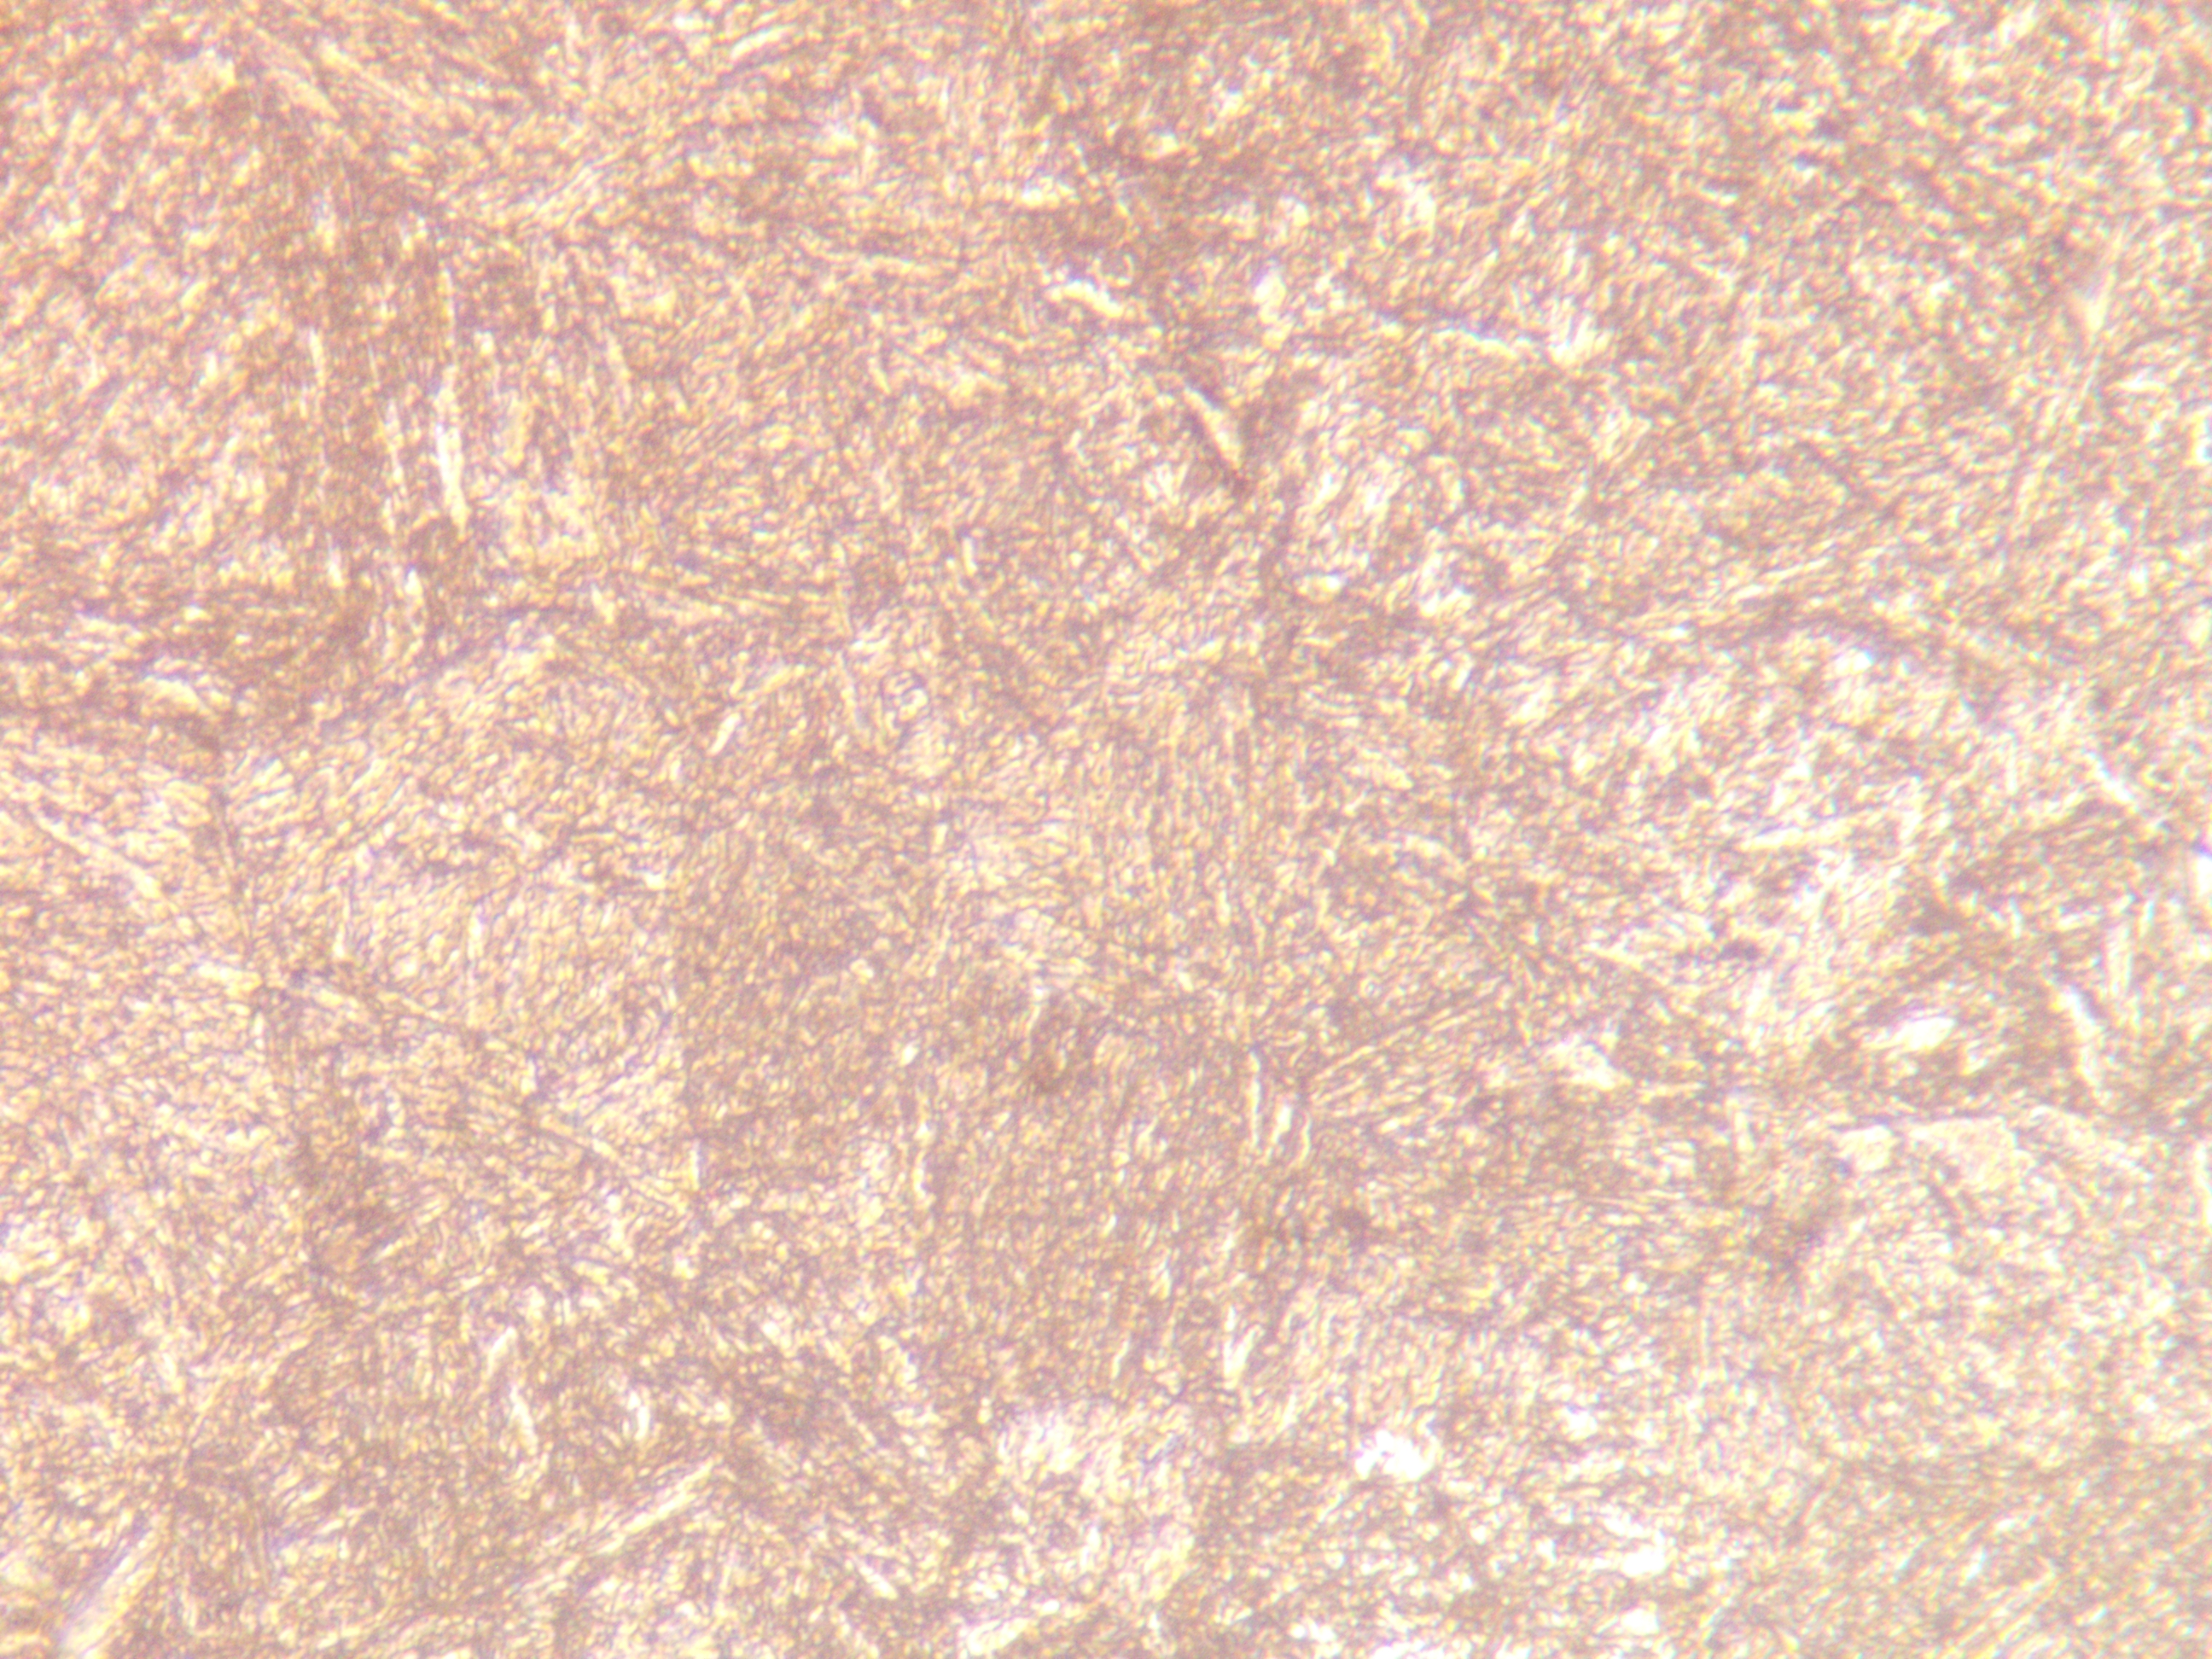
\includegraphics[width=50mm]{21-500.jpg}}
        \ffigbox[50mm]{\caption{21}}{
\includegraphics[width=50mm]{5.png}}
            
    \end{floatrow}

\end{figure}

9.\#22,45钢860°C水淬+高温回火

如图十七,十八,显微组织下呈现回火索氏体的特征,其铁素体基体上分布有细小球(颗粒)状渗碳体。
\begin{figure}[!ht]
    \begin{floatrow}
        \ffigbox[50mm]{\caption{22-200}}{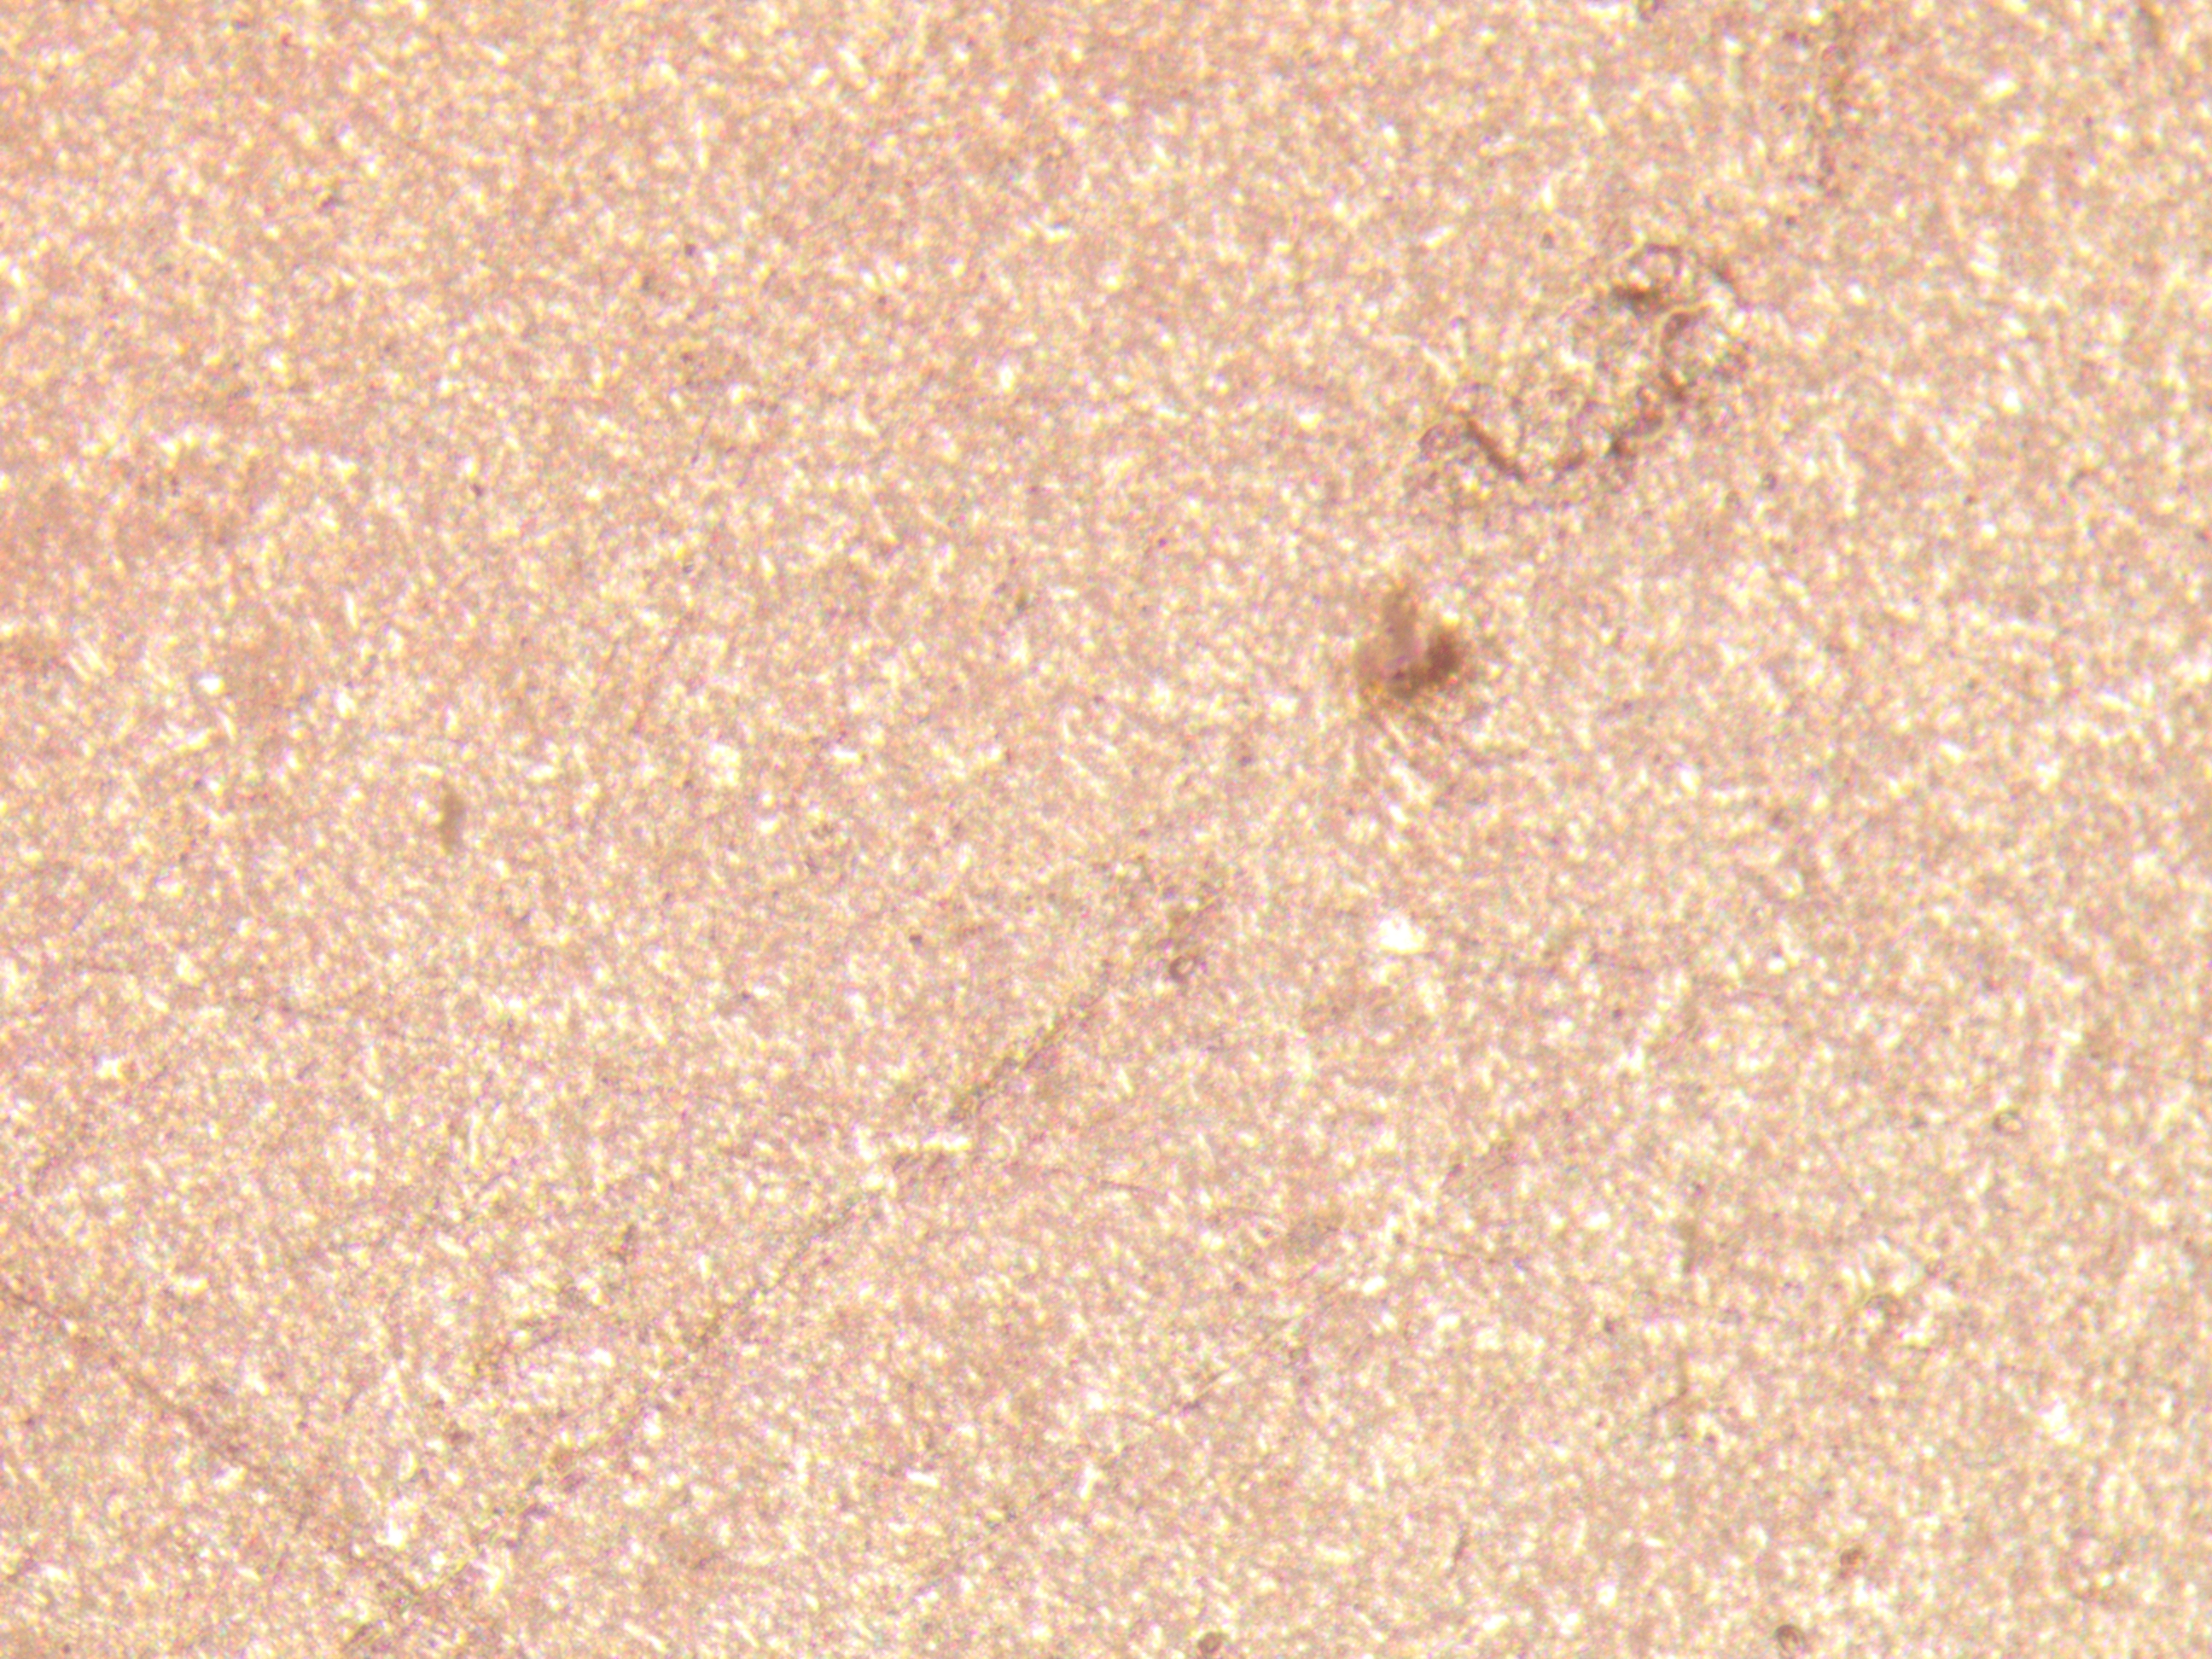
\includegraphics[width=50mm]{22-200.jpg}}
        \ffigbox[50mm]{\caption{22-500}}{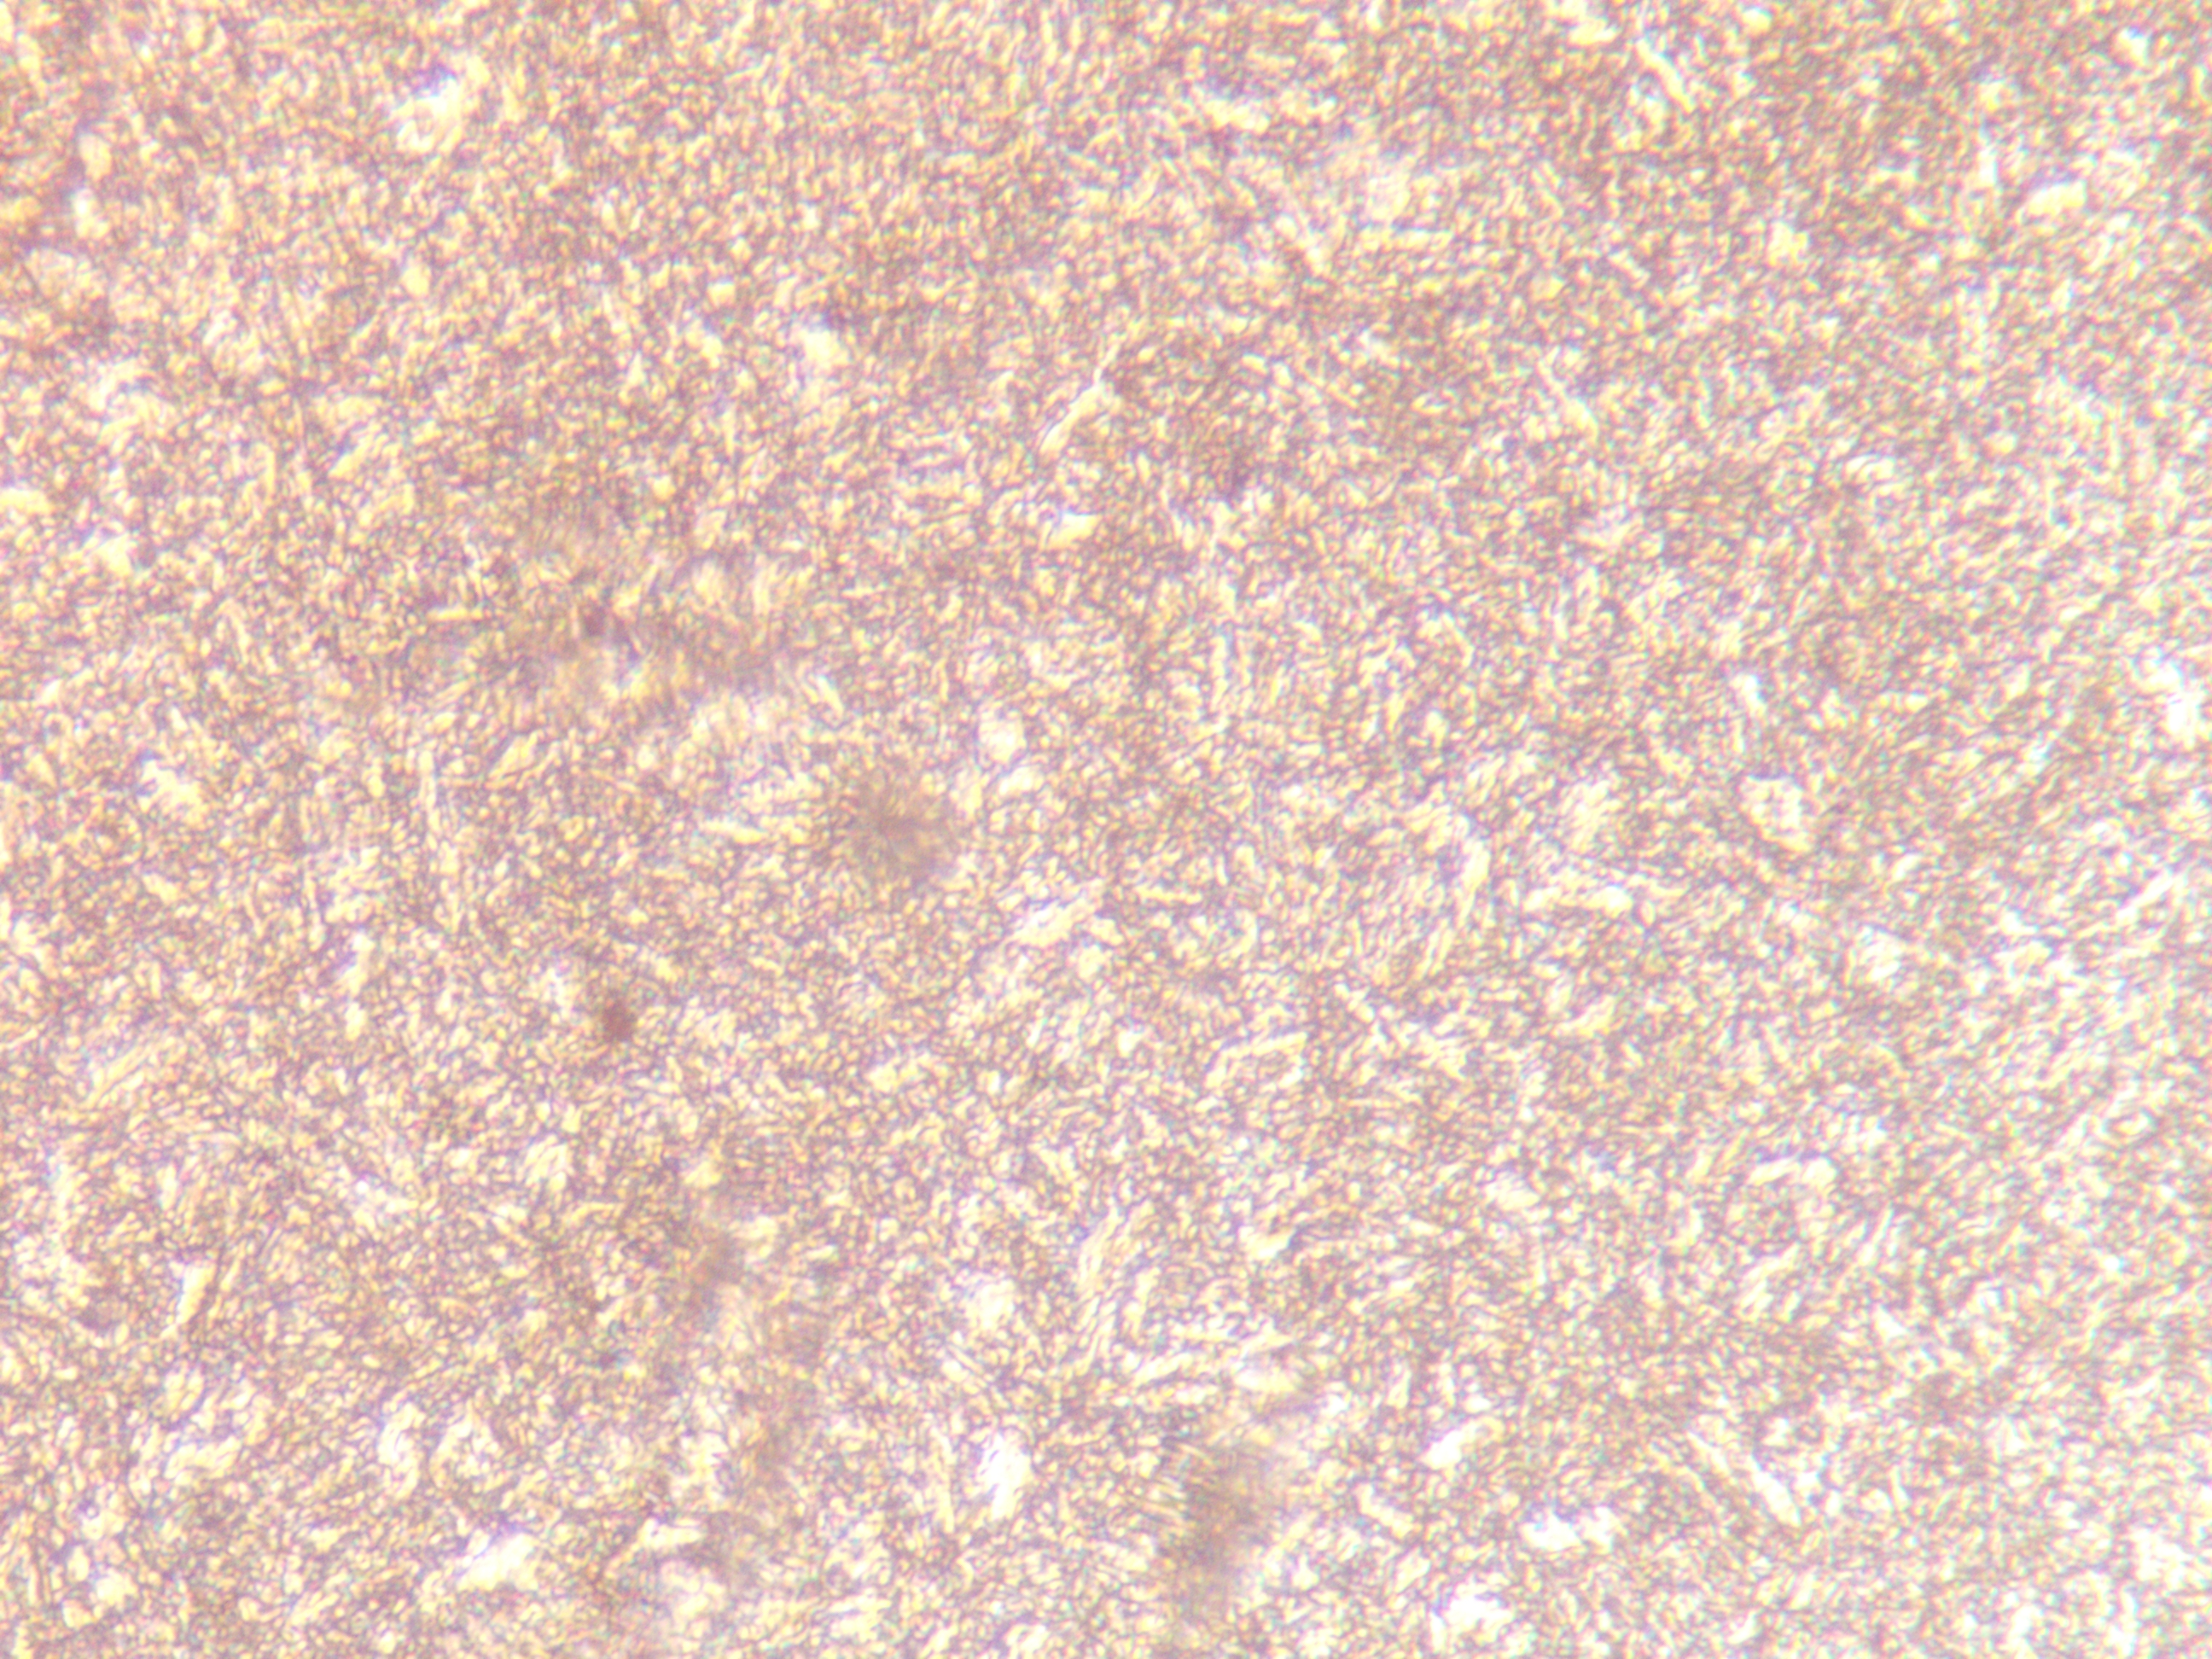
\includegraphics[width=50mm]{22-500.jpg}}
        \ffigbox[50mm]{\caption{22}}{
\includegraphics[width=50mm]{5.png}}
            
    \end{floatrow}

\end{figure}

10.\#23,45钢780°C水淬

如图十九,二十,从500倍可知,白色部分为铁素体,黑色部分为片状的马氏体,结构呈现为片状马氏体和白色不规则小块状铁素体
\begin{figure}[!ht]
    \begin{floatrow}
        \ffigbox[50mm]{\caption{23-200}}{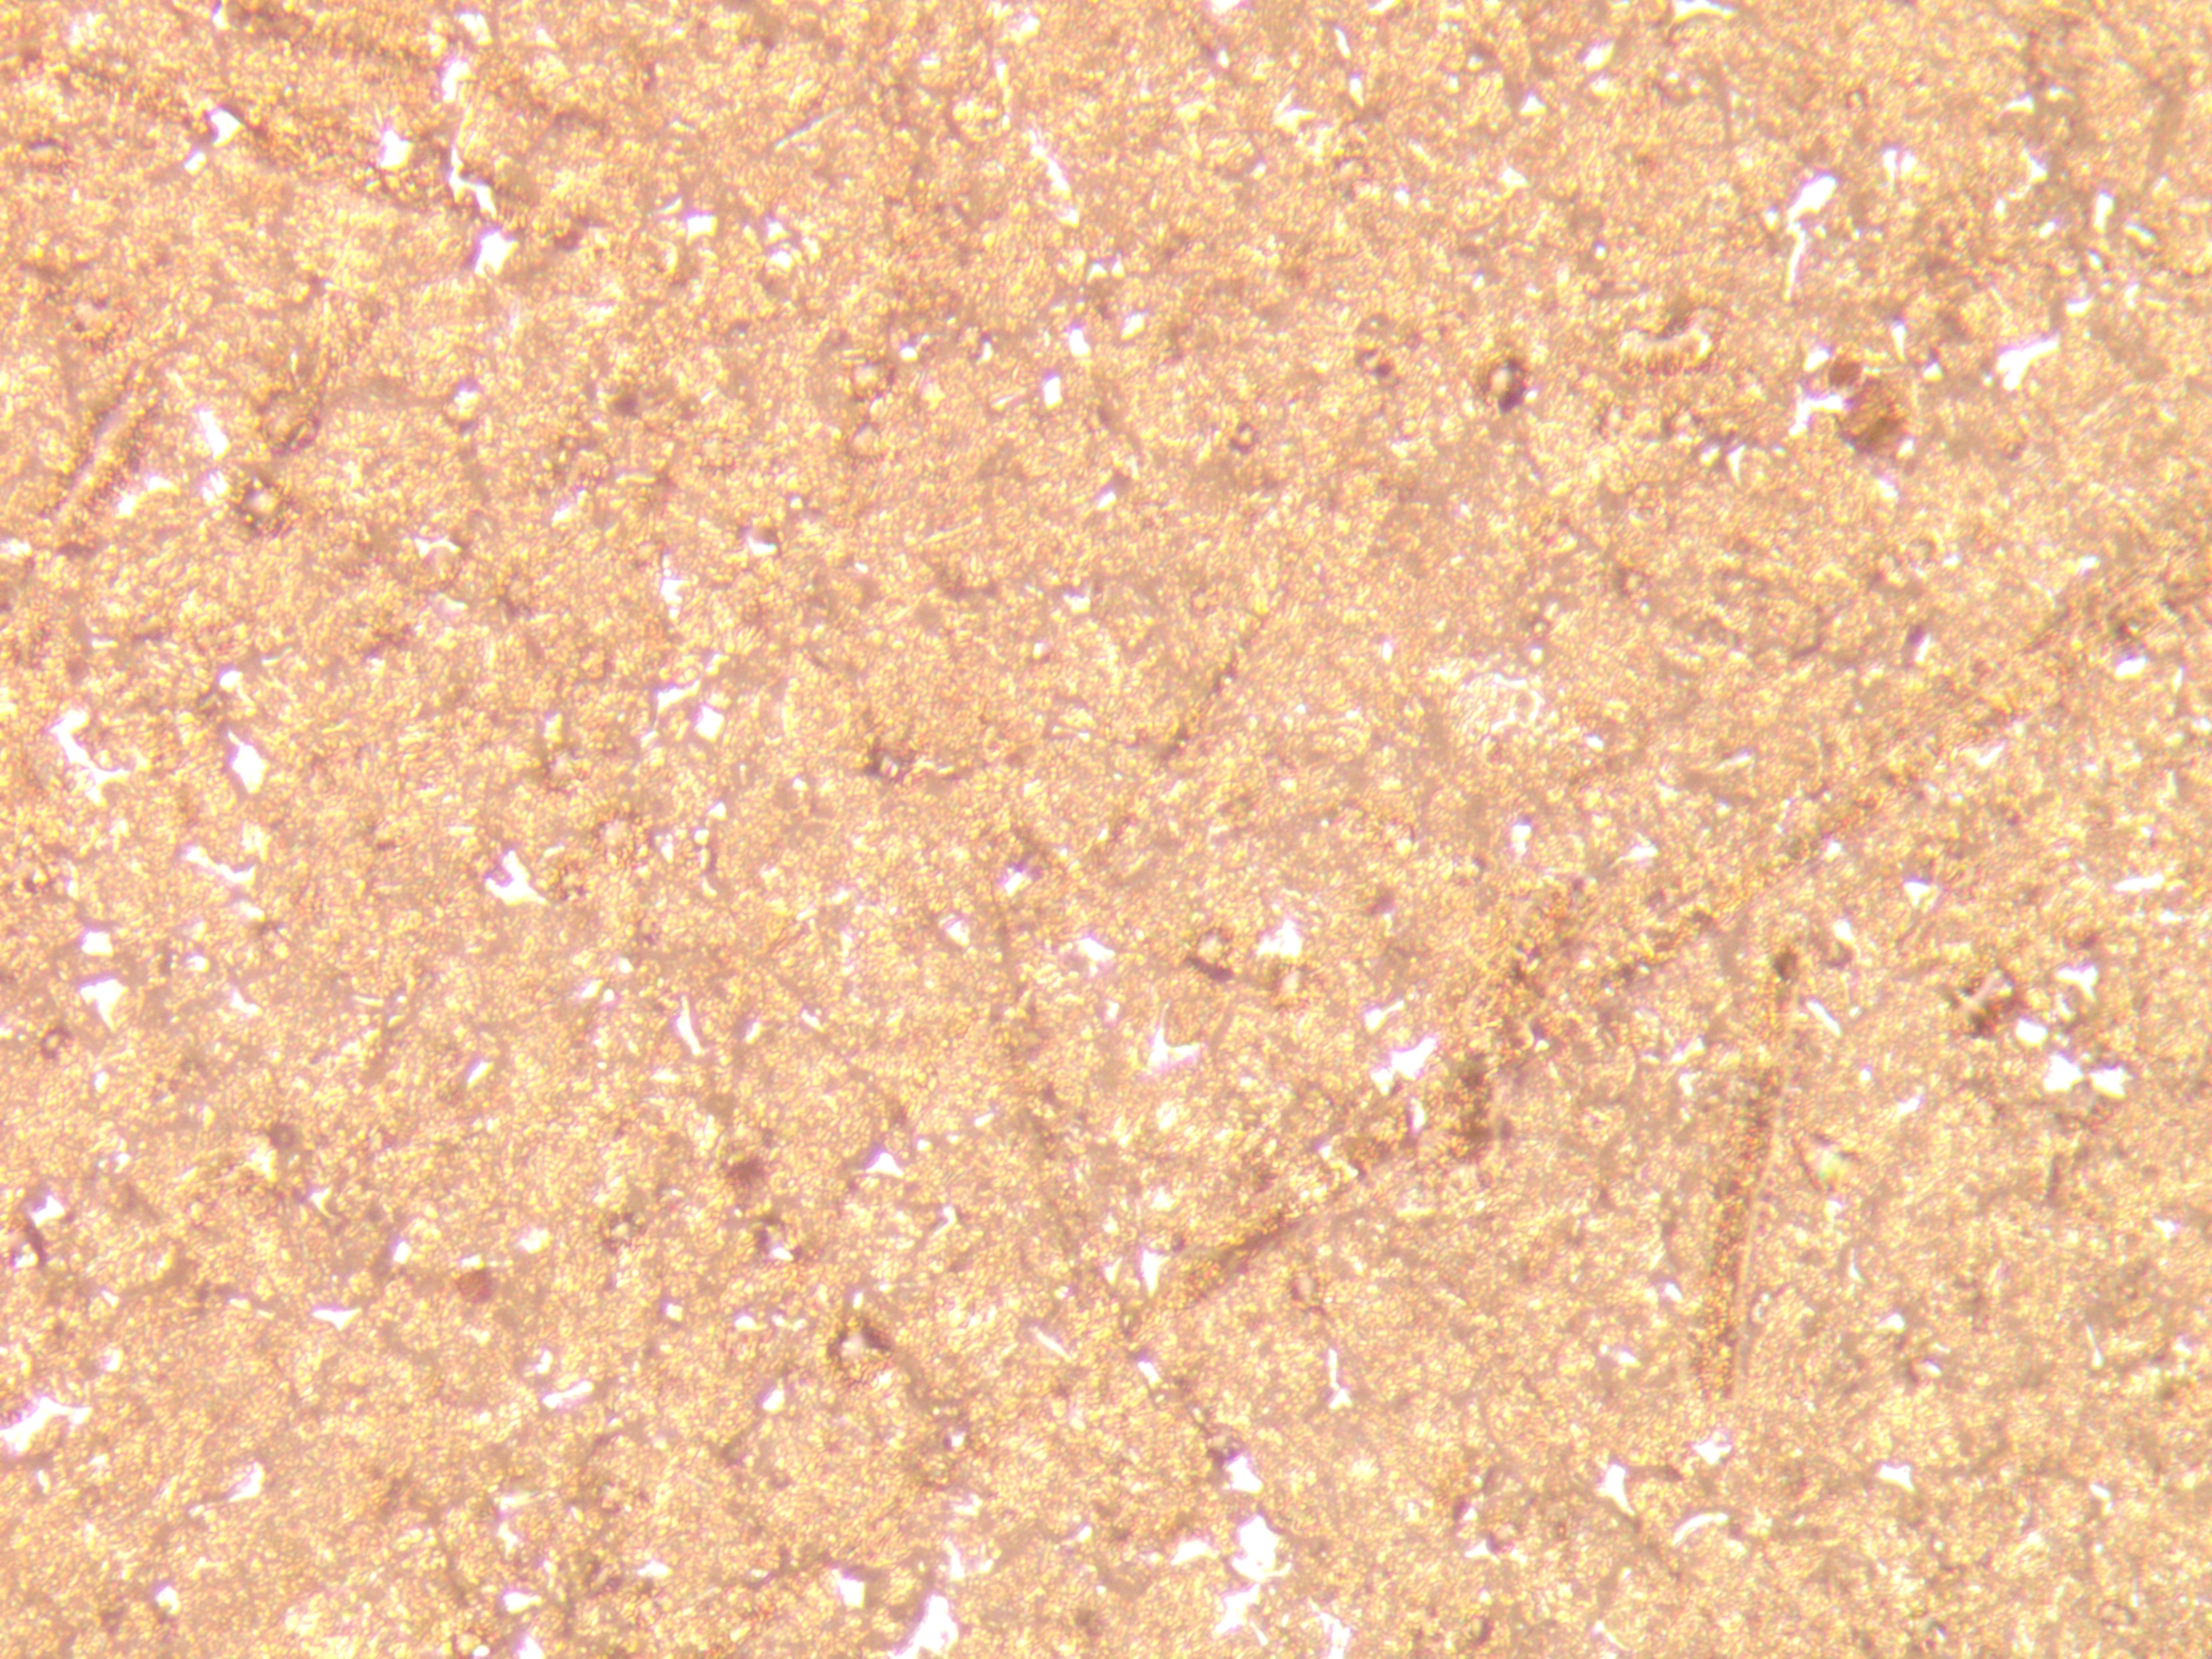
\includegraphics[width=50mm]{23-200.jpg}}
        \ffigbox[50mm]{\caption{23-500}}{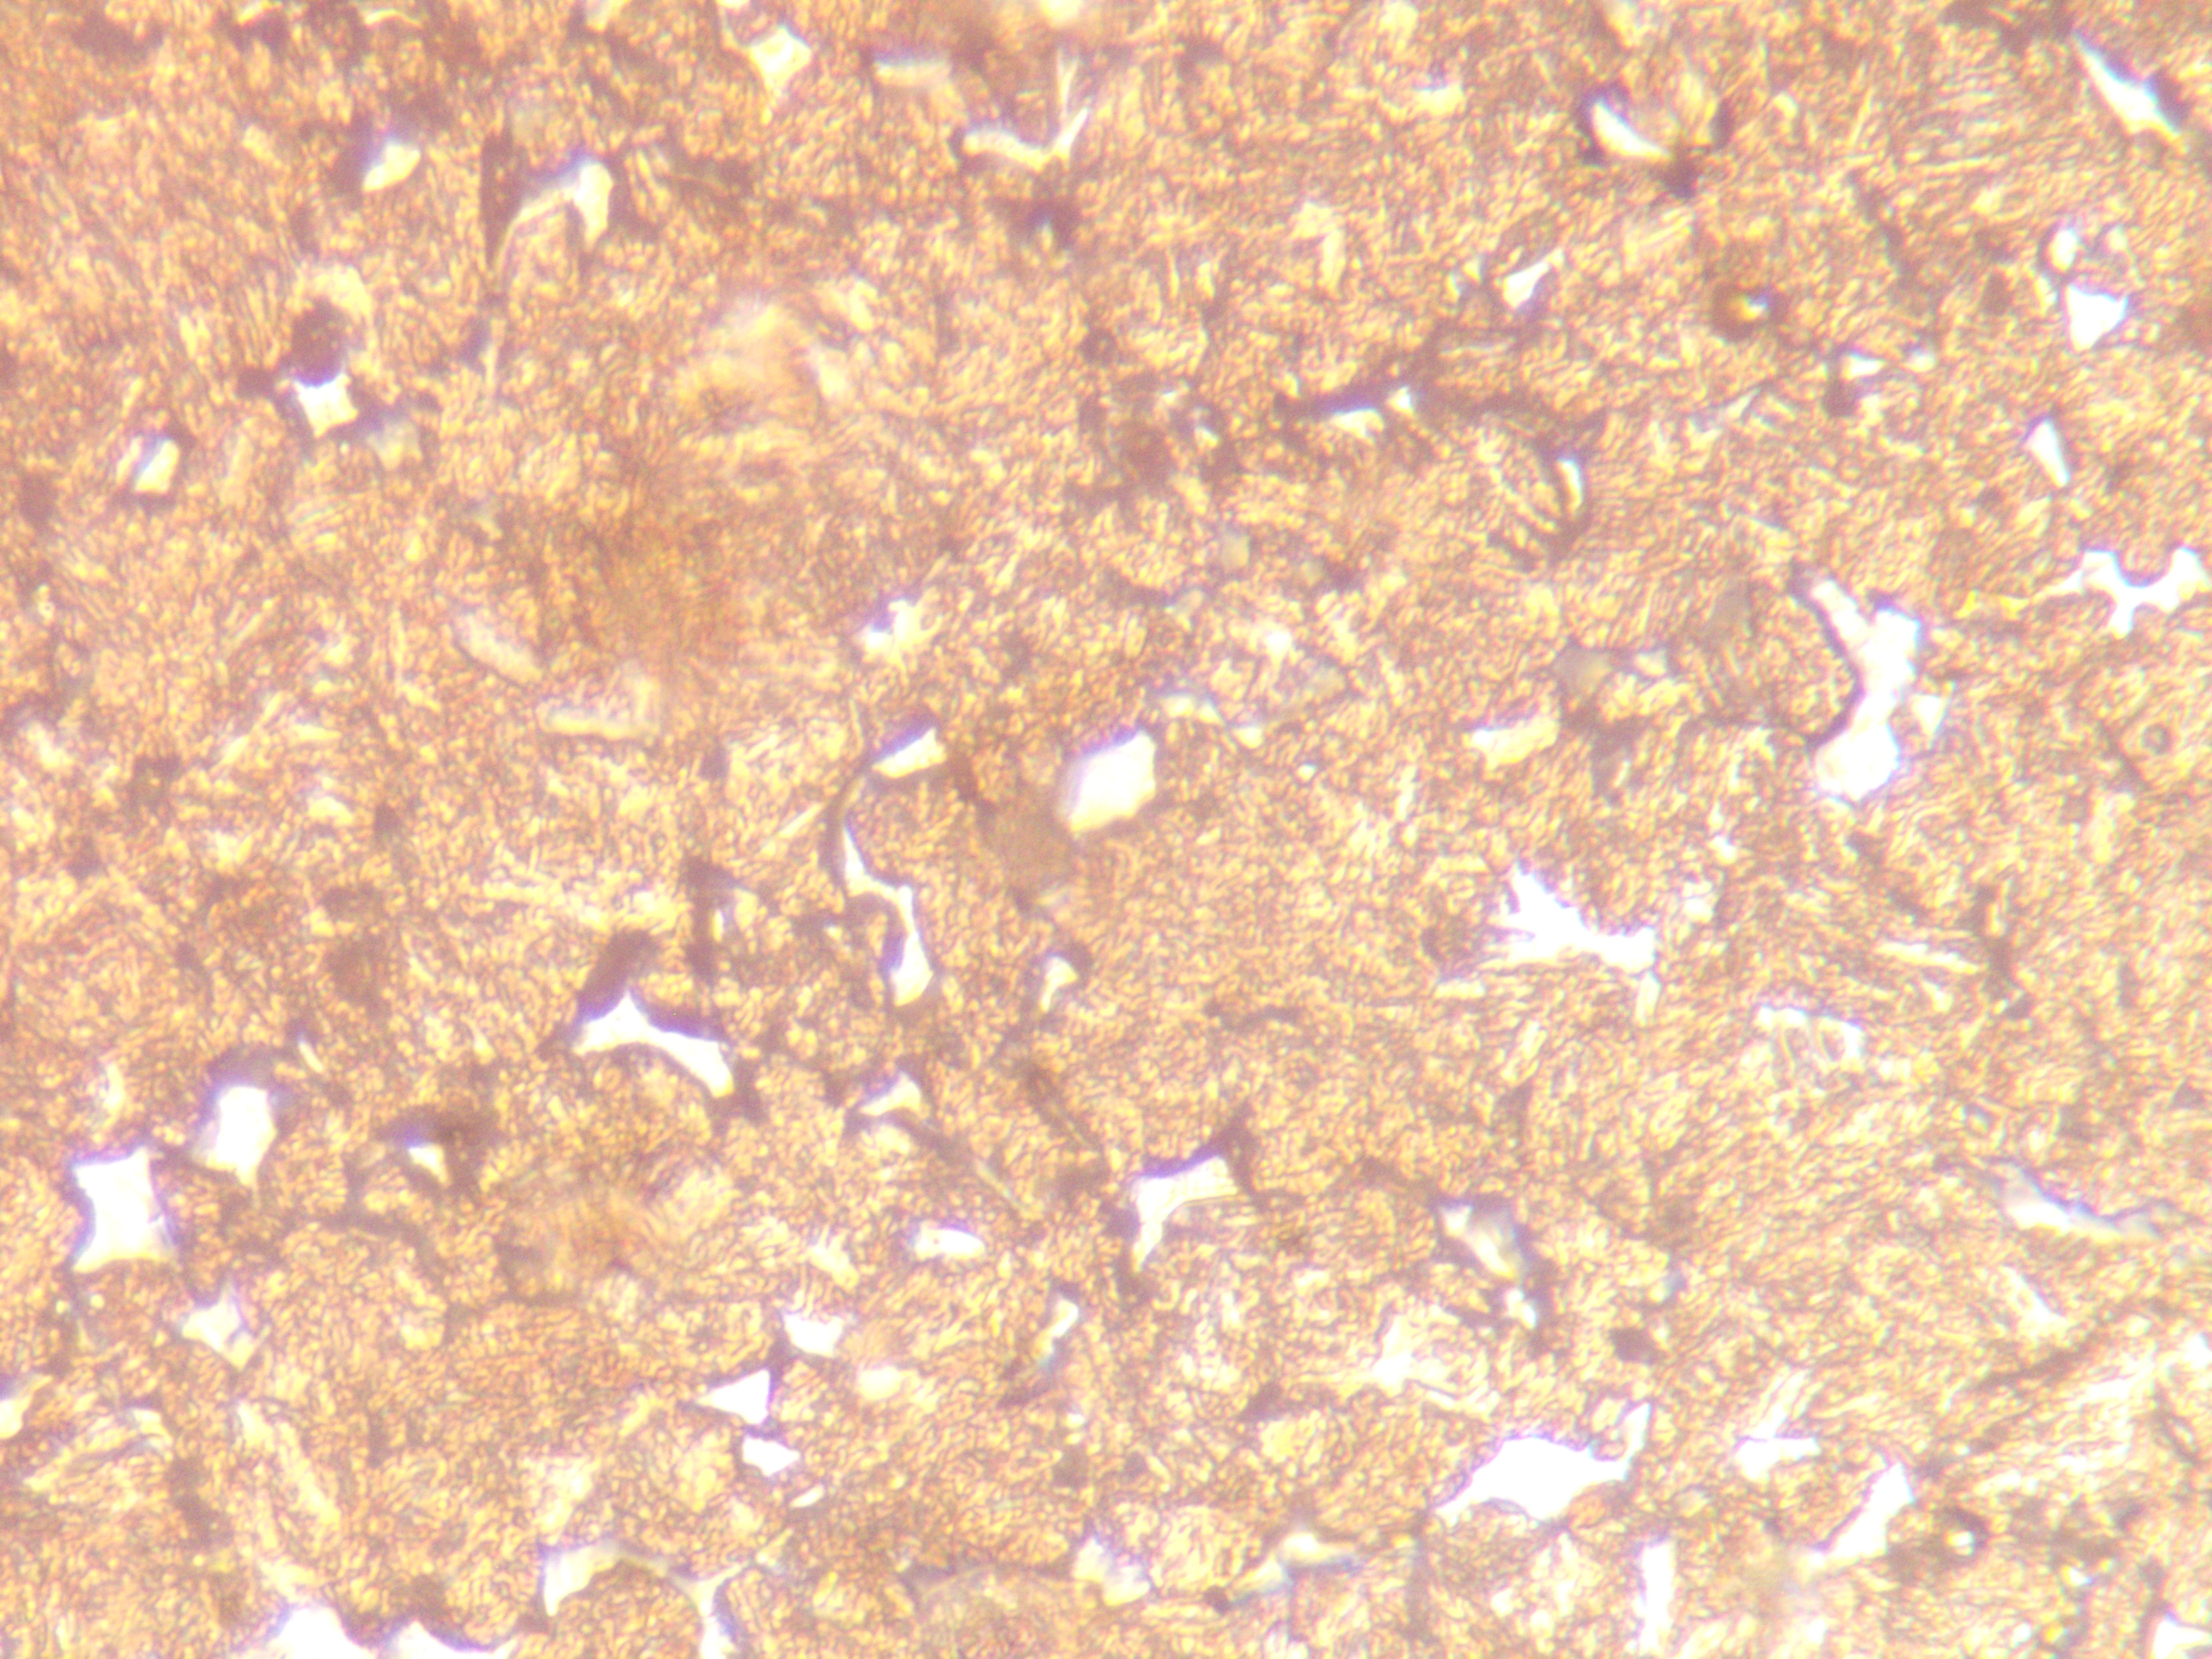
\includegraphics[width=50mm]{23-500.jpg}}
        \ffigbox[50mm]{\caption{23}}{
\includegraphics[width=50mm]{5.png}}
            
    \end{floatrow}

\end{figure}

\newpage
11.\#24,45钢1100°C水淬

如图二十一,二十二,显微组织下的结构呈现为珠光体。在200倍显微镜下,观察到的一条条黑线是渗碳体,
500倍显微镜下,观察到宽条的铁素体和细条的渗碳体。
\begin{figure}[!ht]
    \begin{floatrow}
        \ffigbox[50mm]{\caption{24-200}}{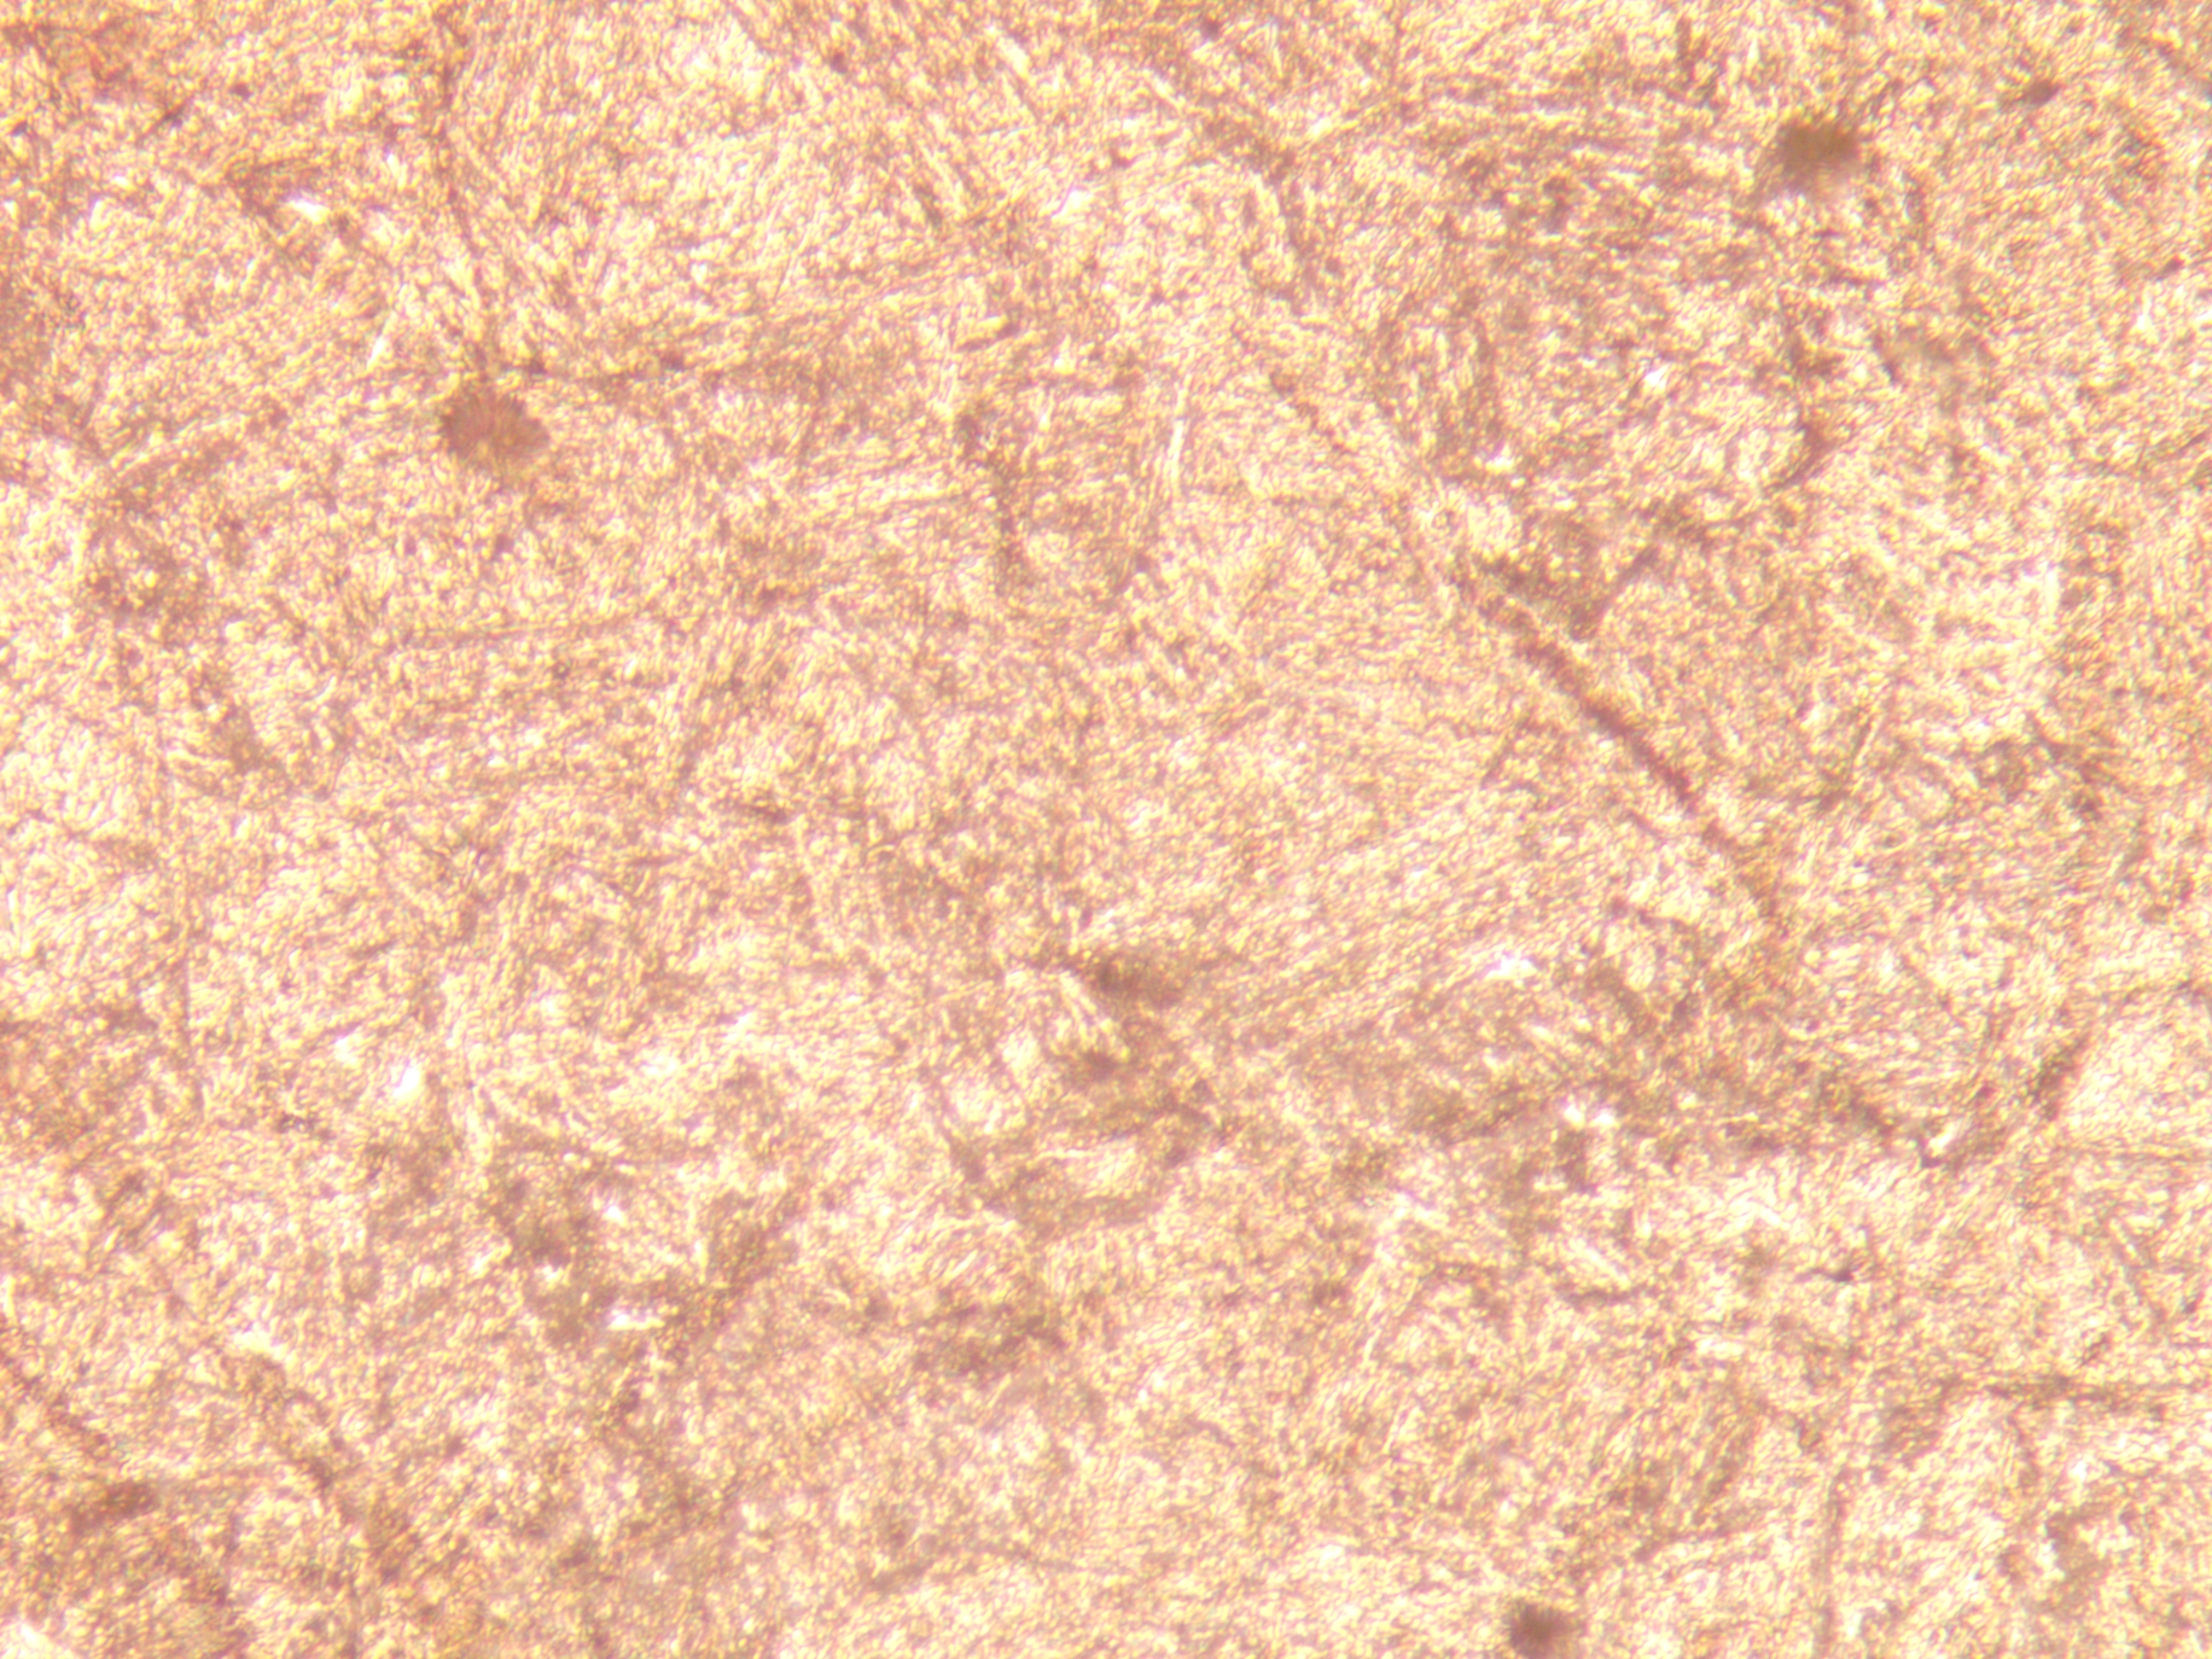
\includegraphics[width=50mm]{24-200.jpg}}
        \ffigbox[50mm]{\caption{24-500}}{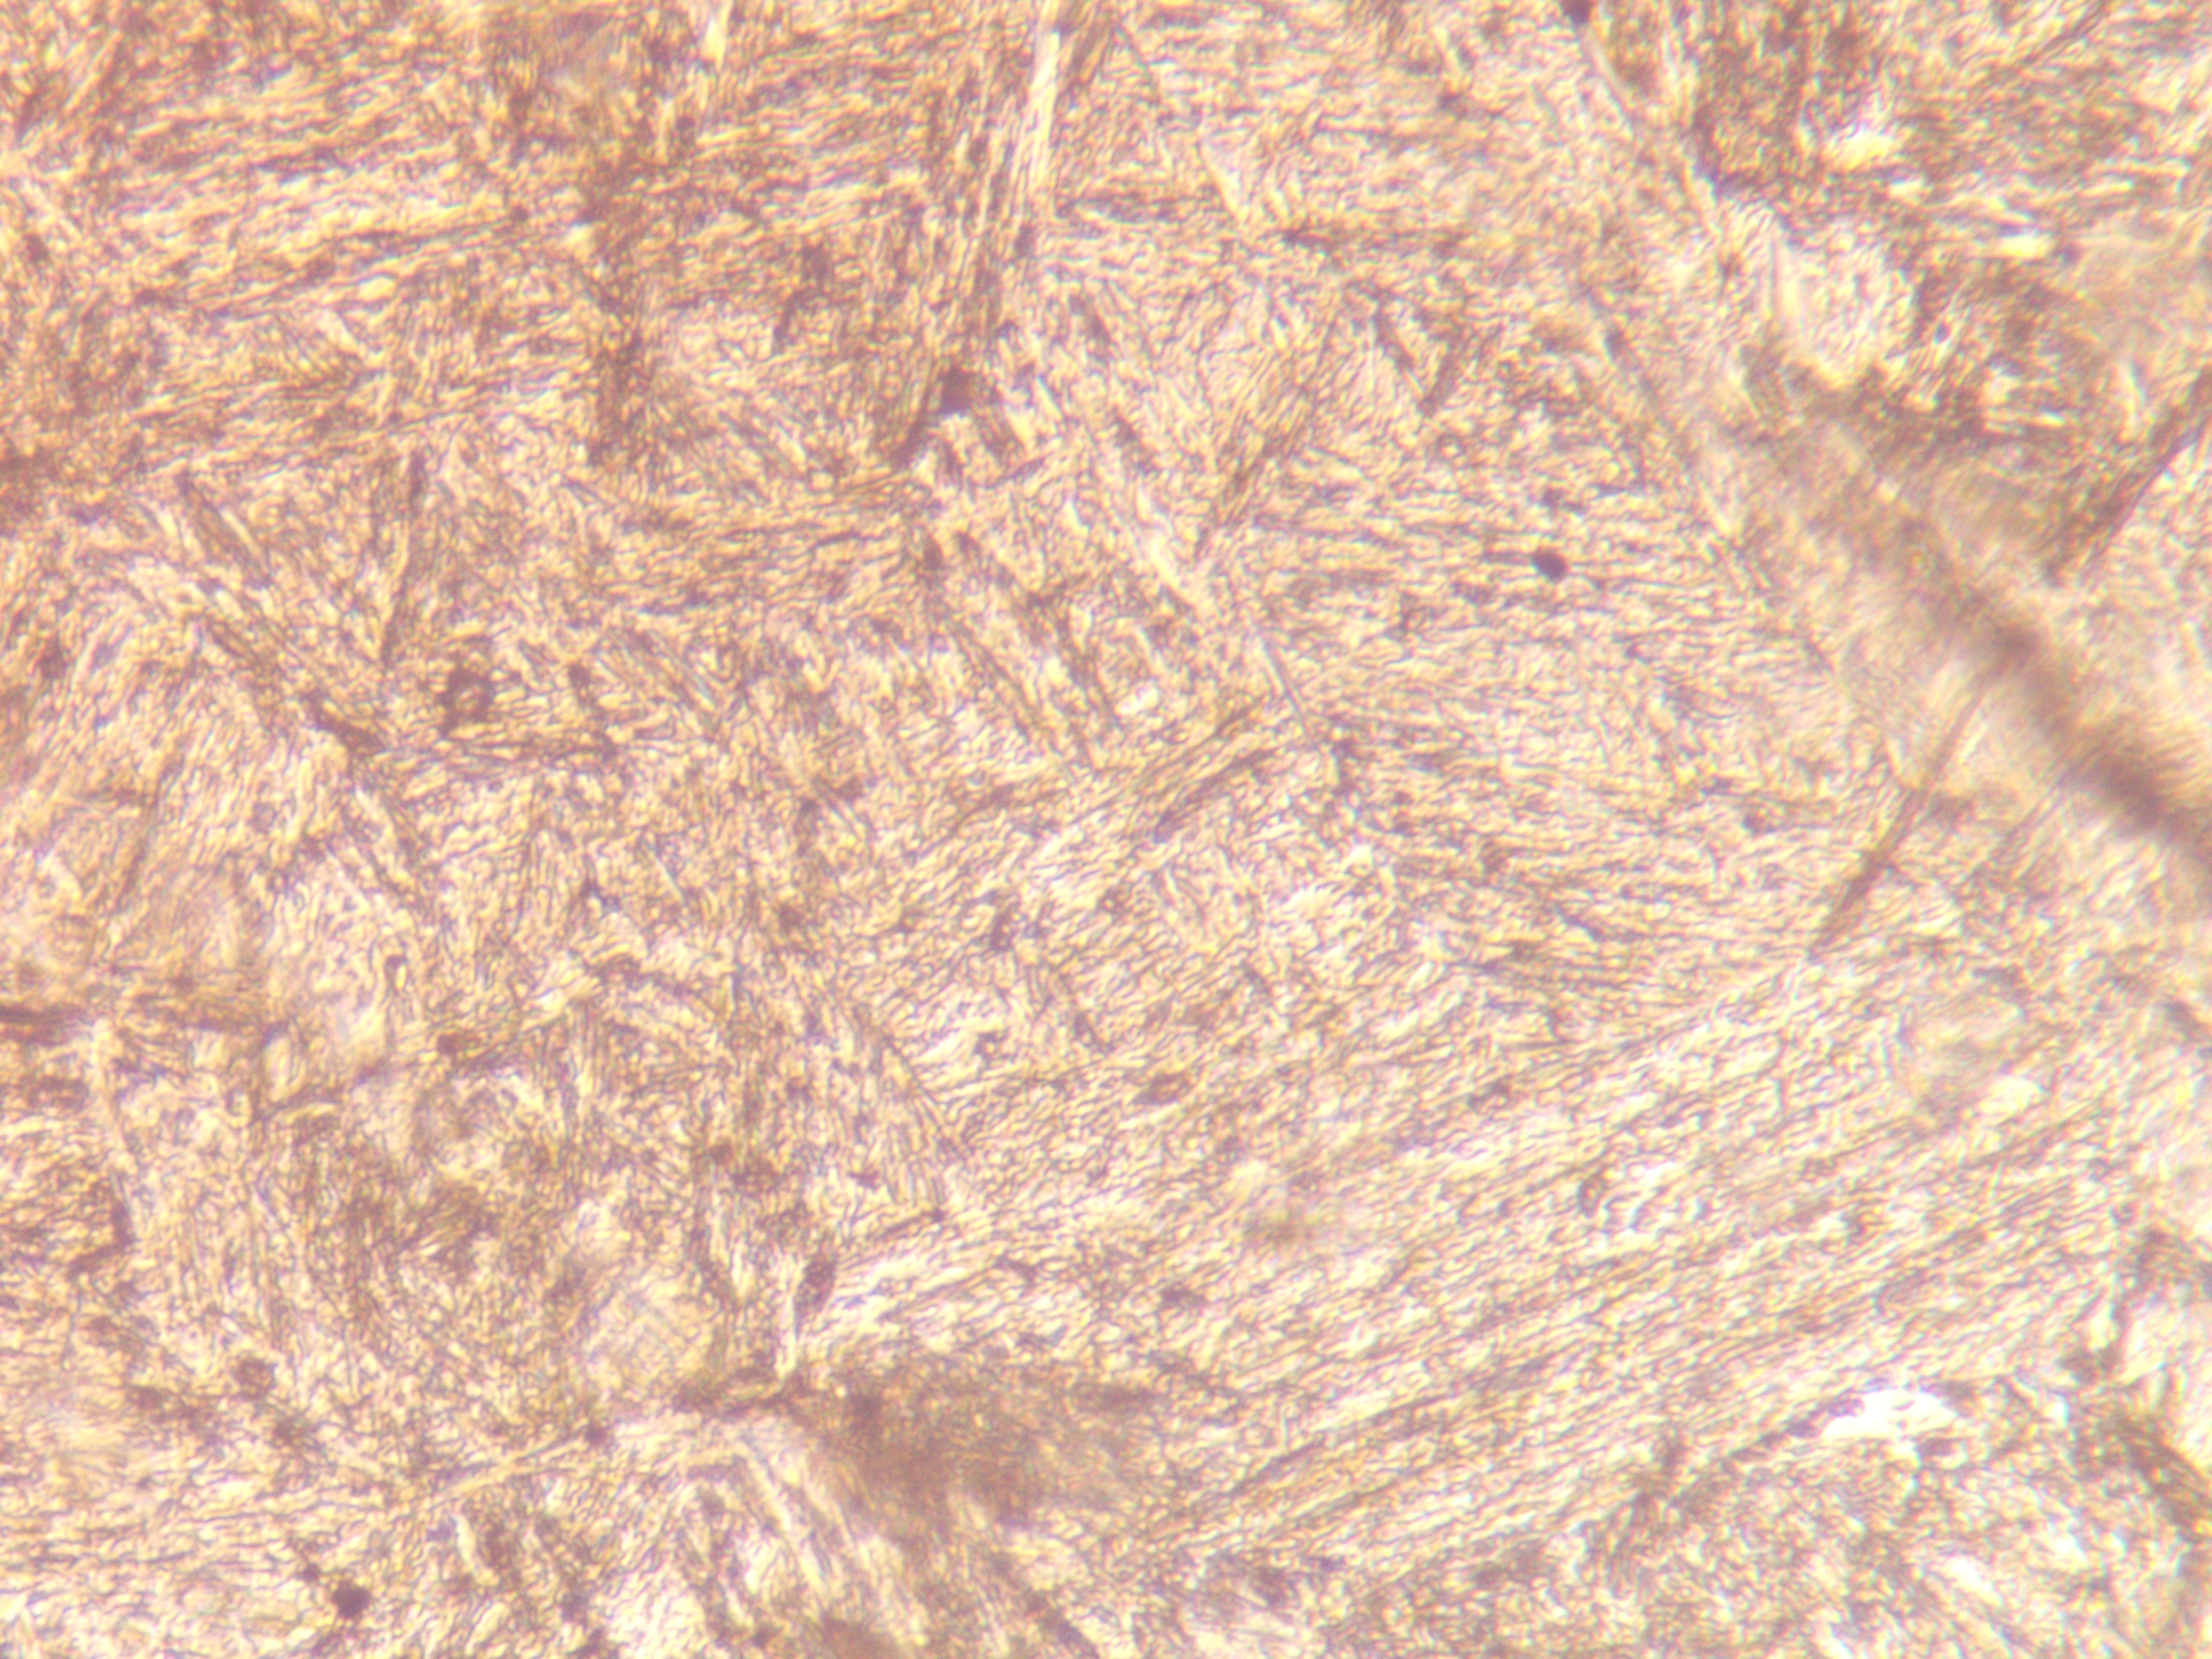
\includegraphics[width=50mm]{24-500.jpg}}
        \ffigbox[50mm]{\caption{24}}{
\includegraphics[width=50mm]{5.png}}
            
    \end{floatrow}

\end{figure}

12.\#25,T12钢球化退火


如图二十三,二十四,其结构呈现为回火马氏体的基体上分布着许多不规则的小颗粒状碳三铁。
图中由明显的颜色差异(不是明显的黑白的颜色差距),基体中铁素体晶粒之间的晶界,没有腐蚀出来,观察不到
\begin{figure}[!ht]
    \begin{floatrow}
        \ffigbox[50mm]{\caption{25-200}}{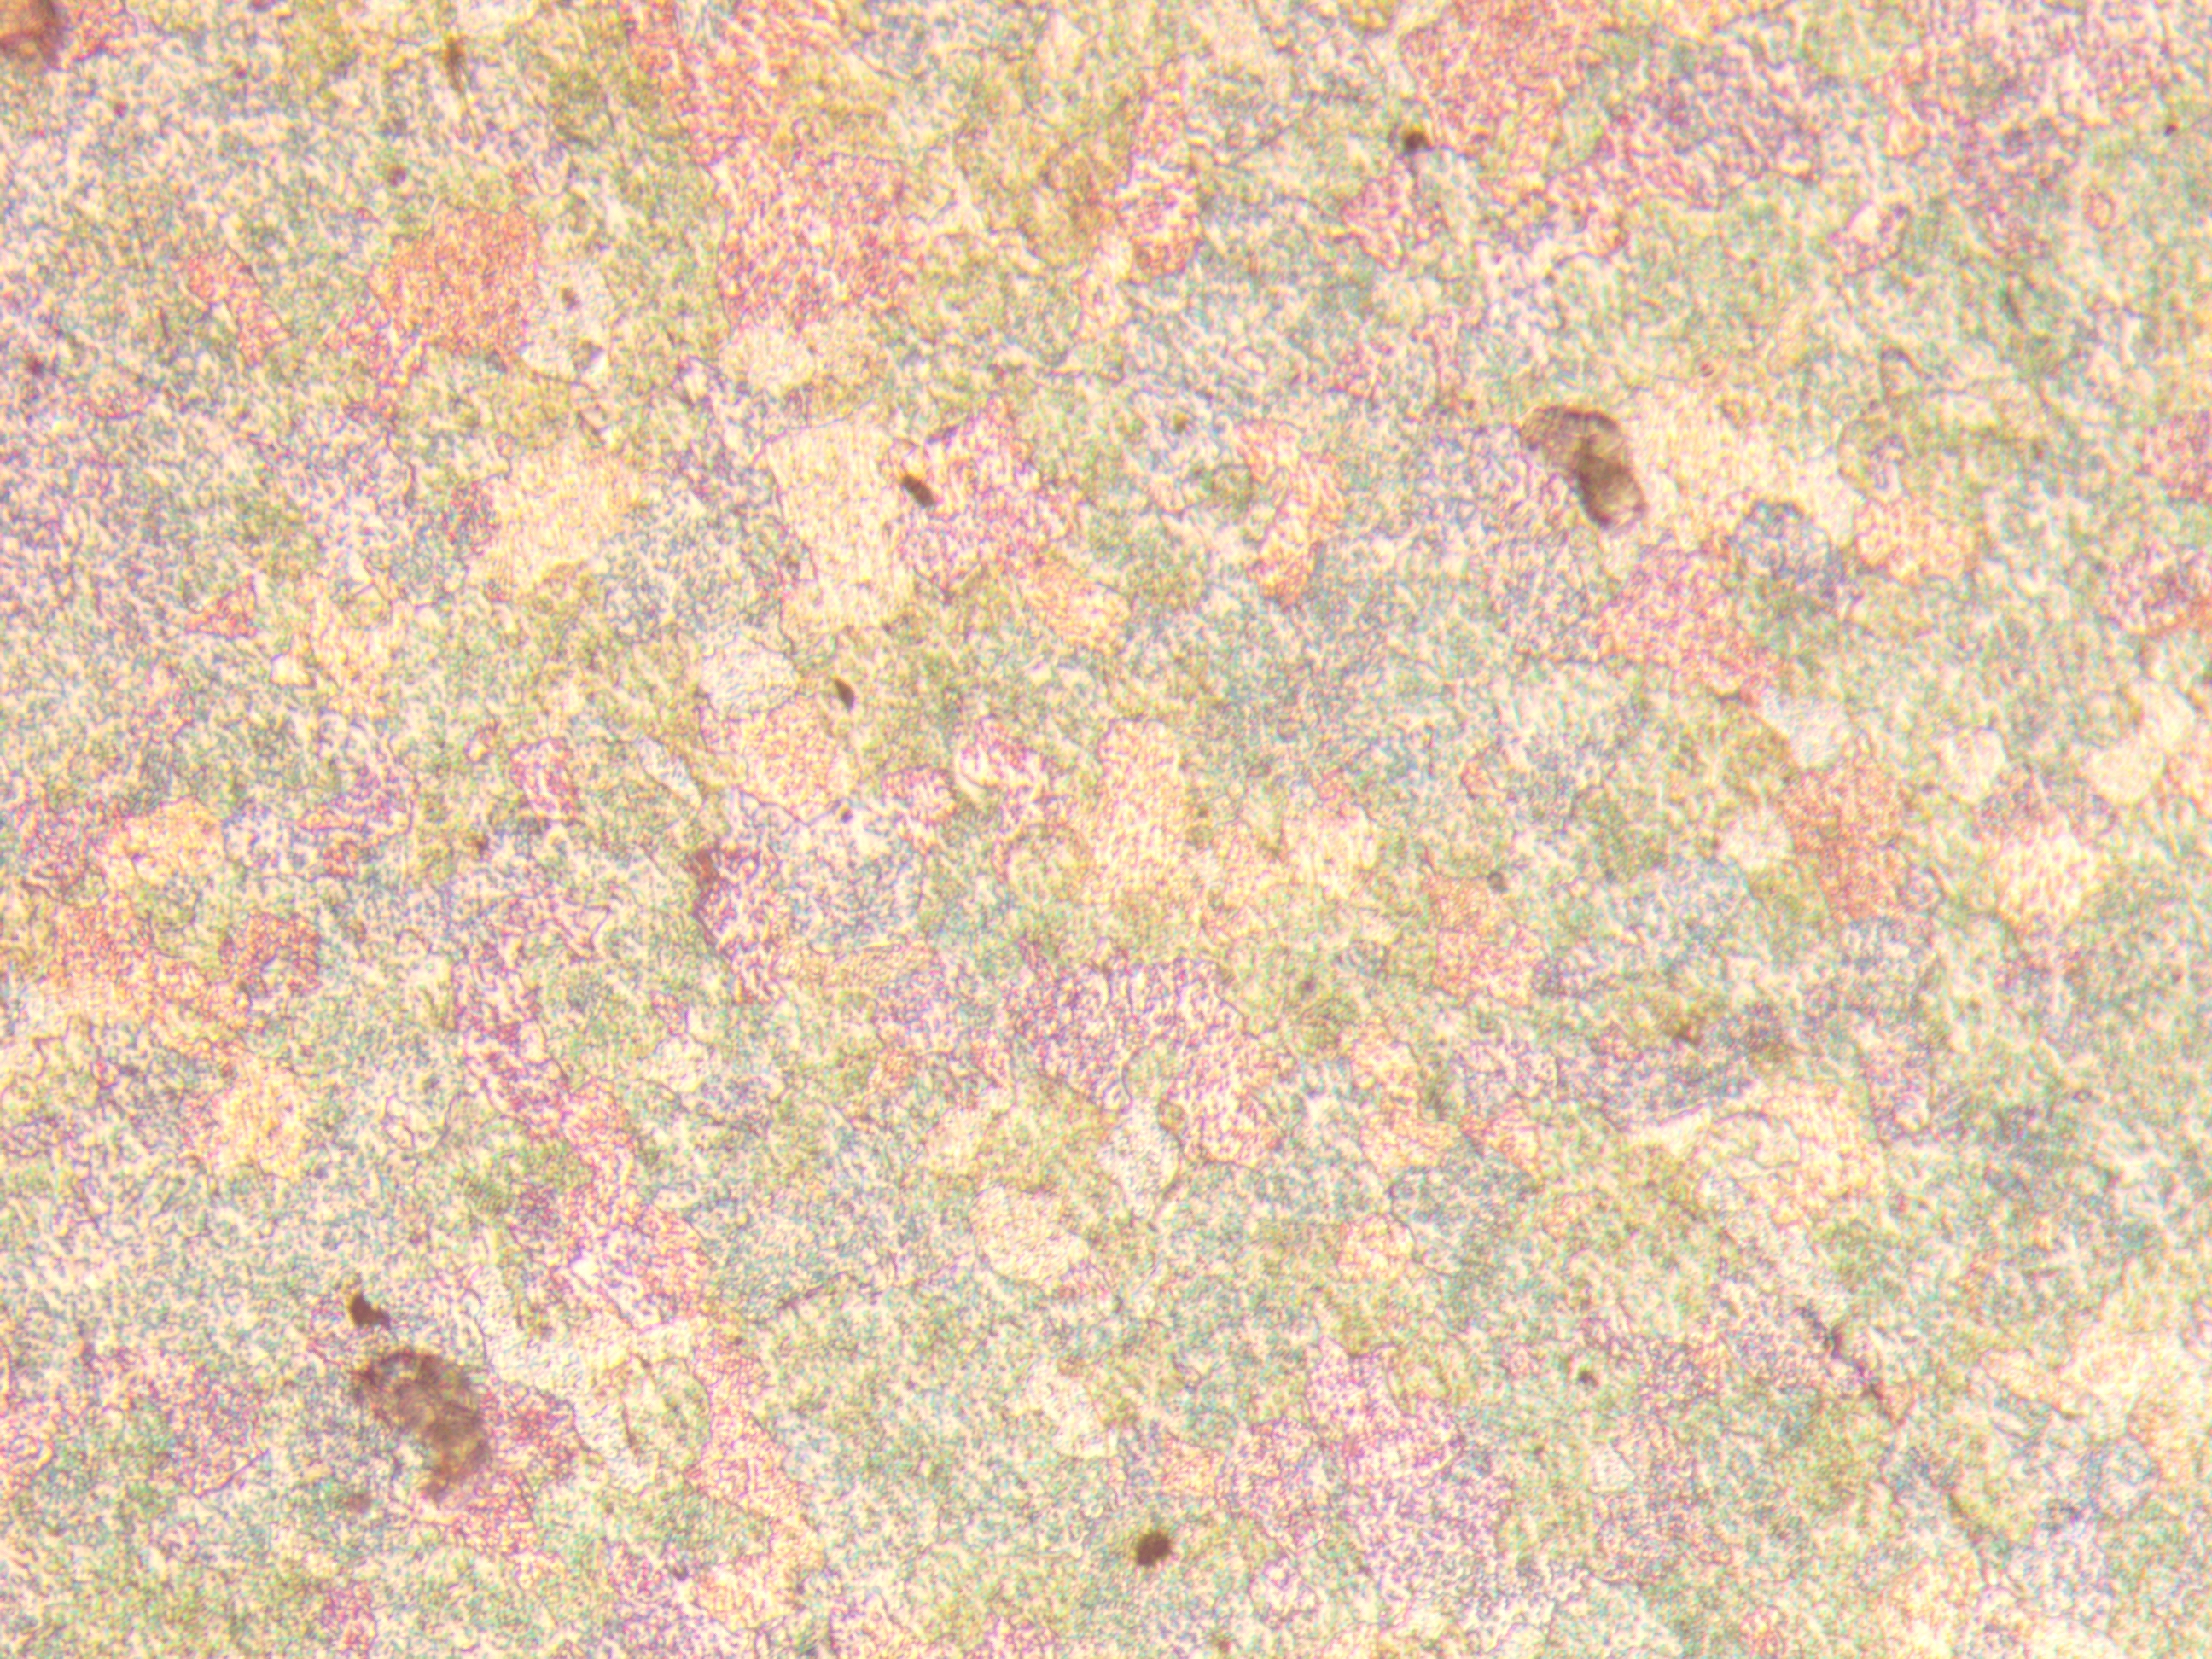
\includegraphics[width=50mm]{25-200.jpg}}
        \ffigbox[50mm]{\caption{25-500}}{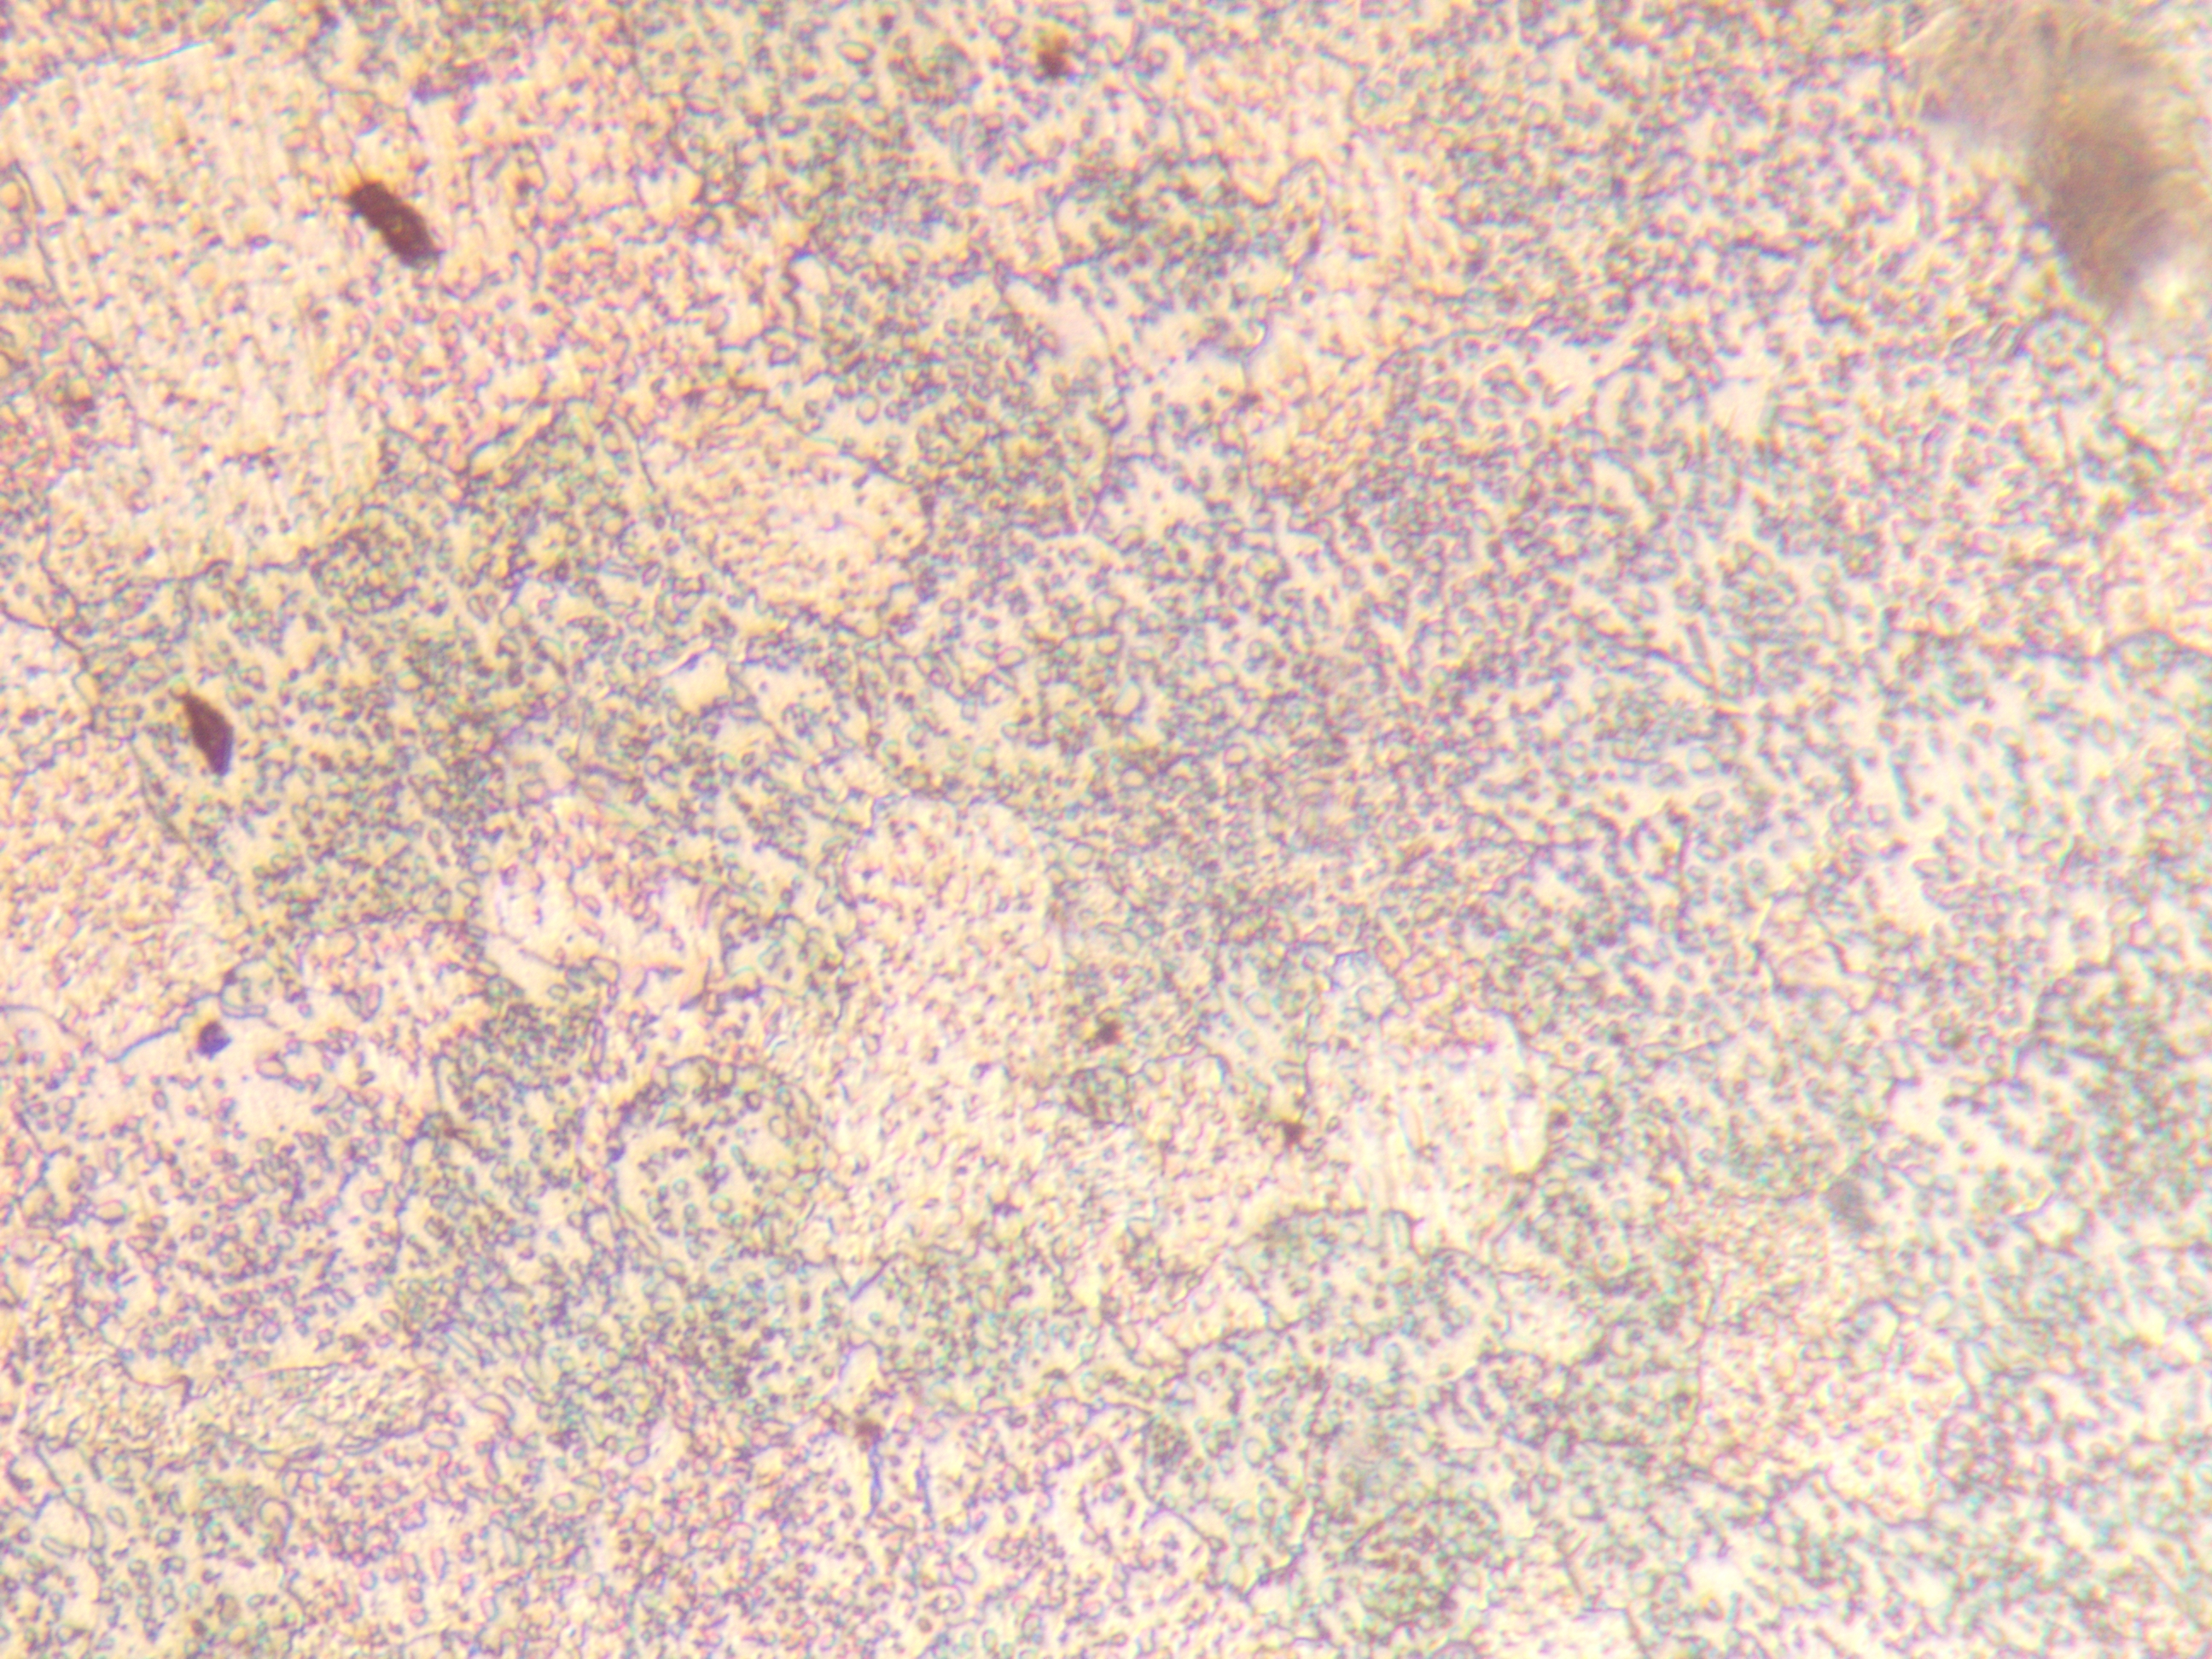
\includegraphics[width=50mm]{25-500.jpg}}
        \ffigbox[50mm]{\caption{25}}{
\includegraphics[width=50mm]{5.png}}
            
    \end{floatrow}

\end{figure}



13.\#26,T12钢780°C水淬+低温回火

如图二十五、二十六,主要结构为回火马氏体,基体上分布着小块颗粒状二次渗碳体。

\begin{figure}[!ht]
    \begin{floatrow}
        \ffigbox[50mm]{\caption{26-200}}{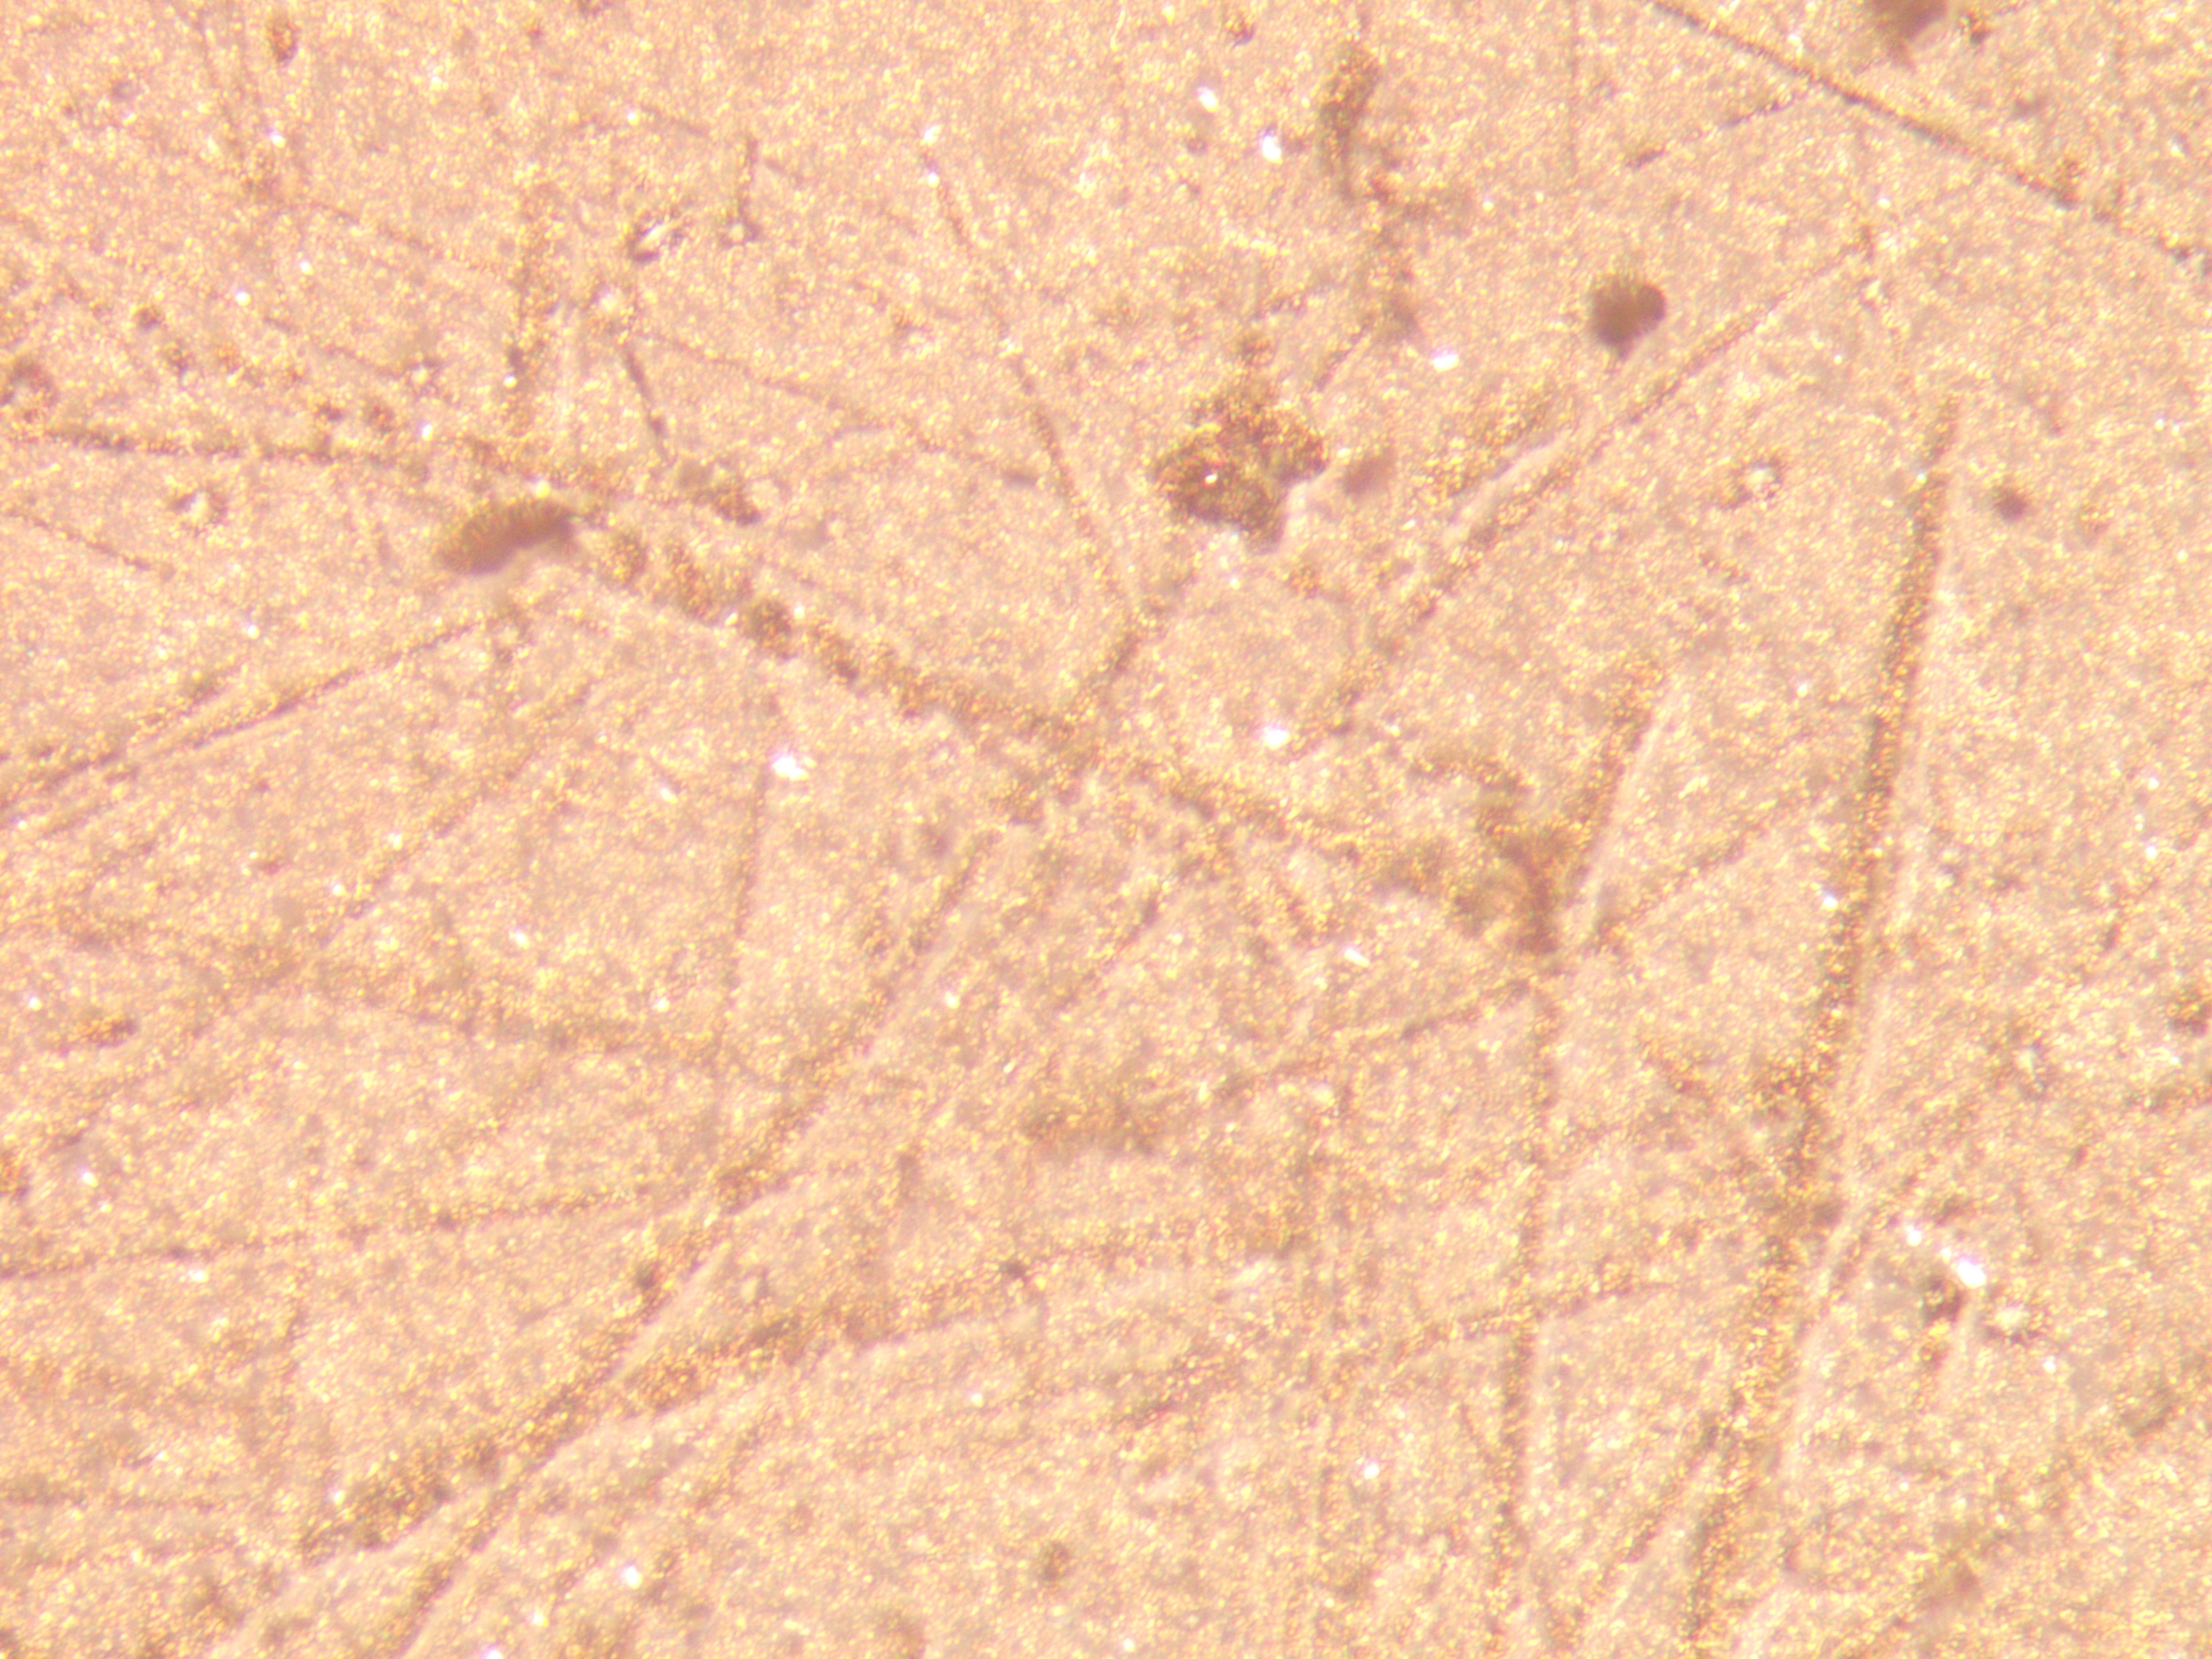
\includegraphics[width=50mm]{26-200.jpg}}
        \ffigbox[50mm]{\caption{26-500}}{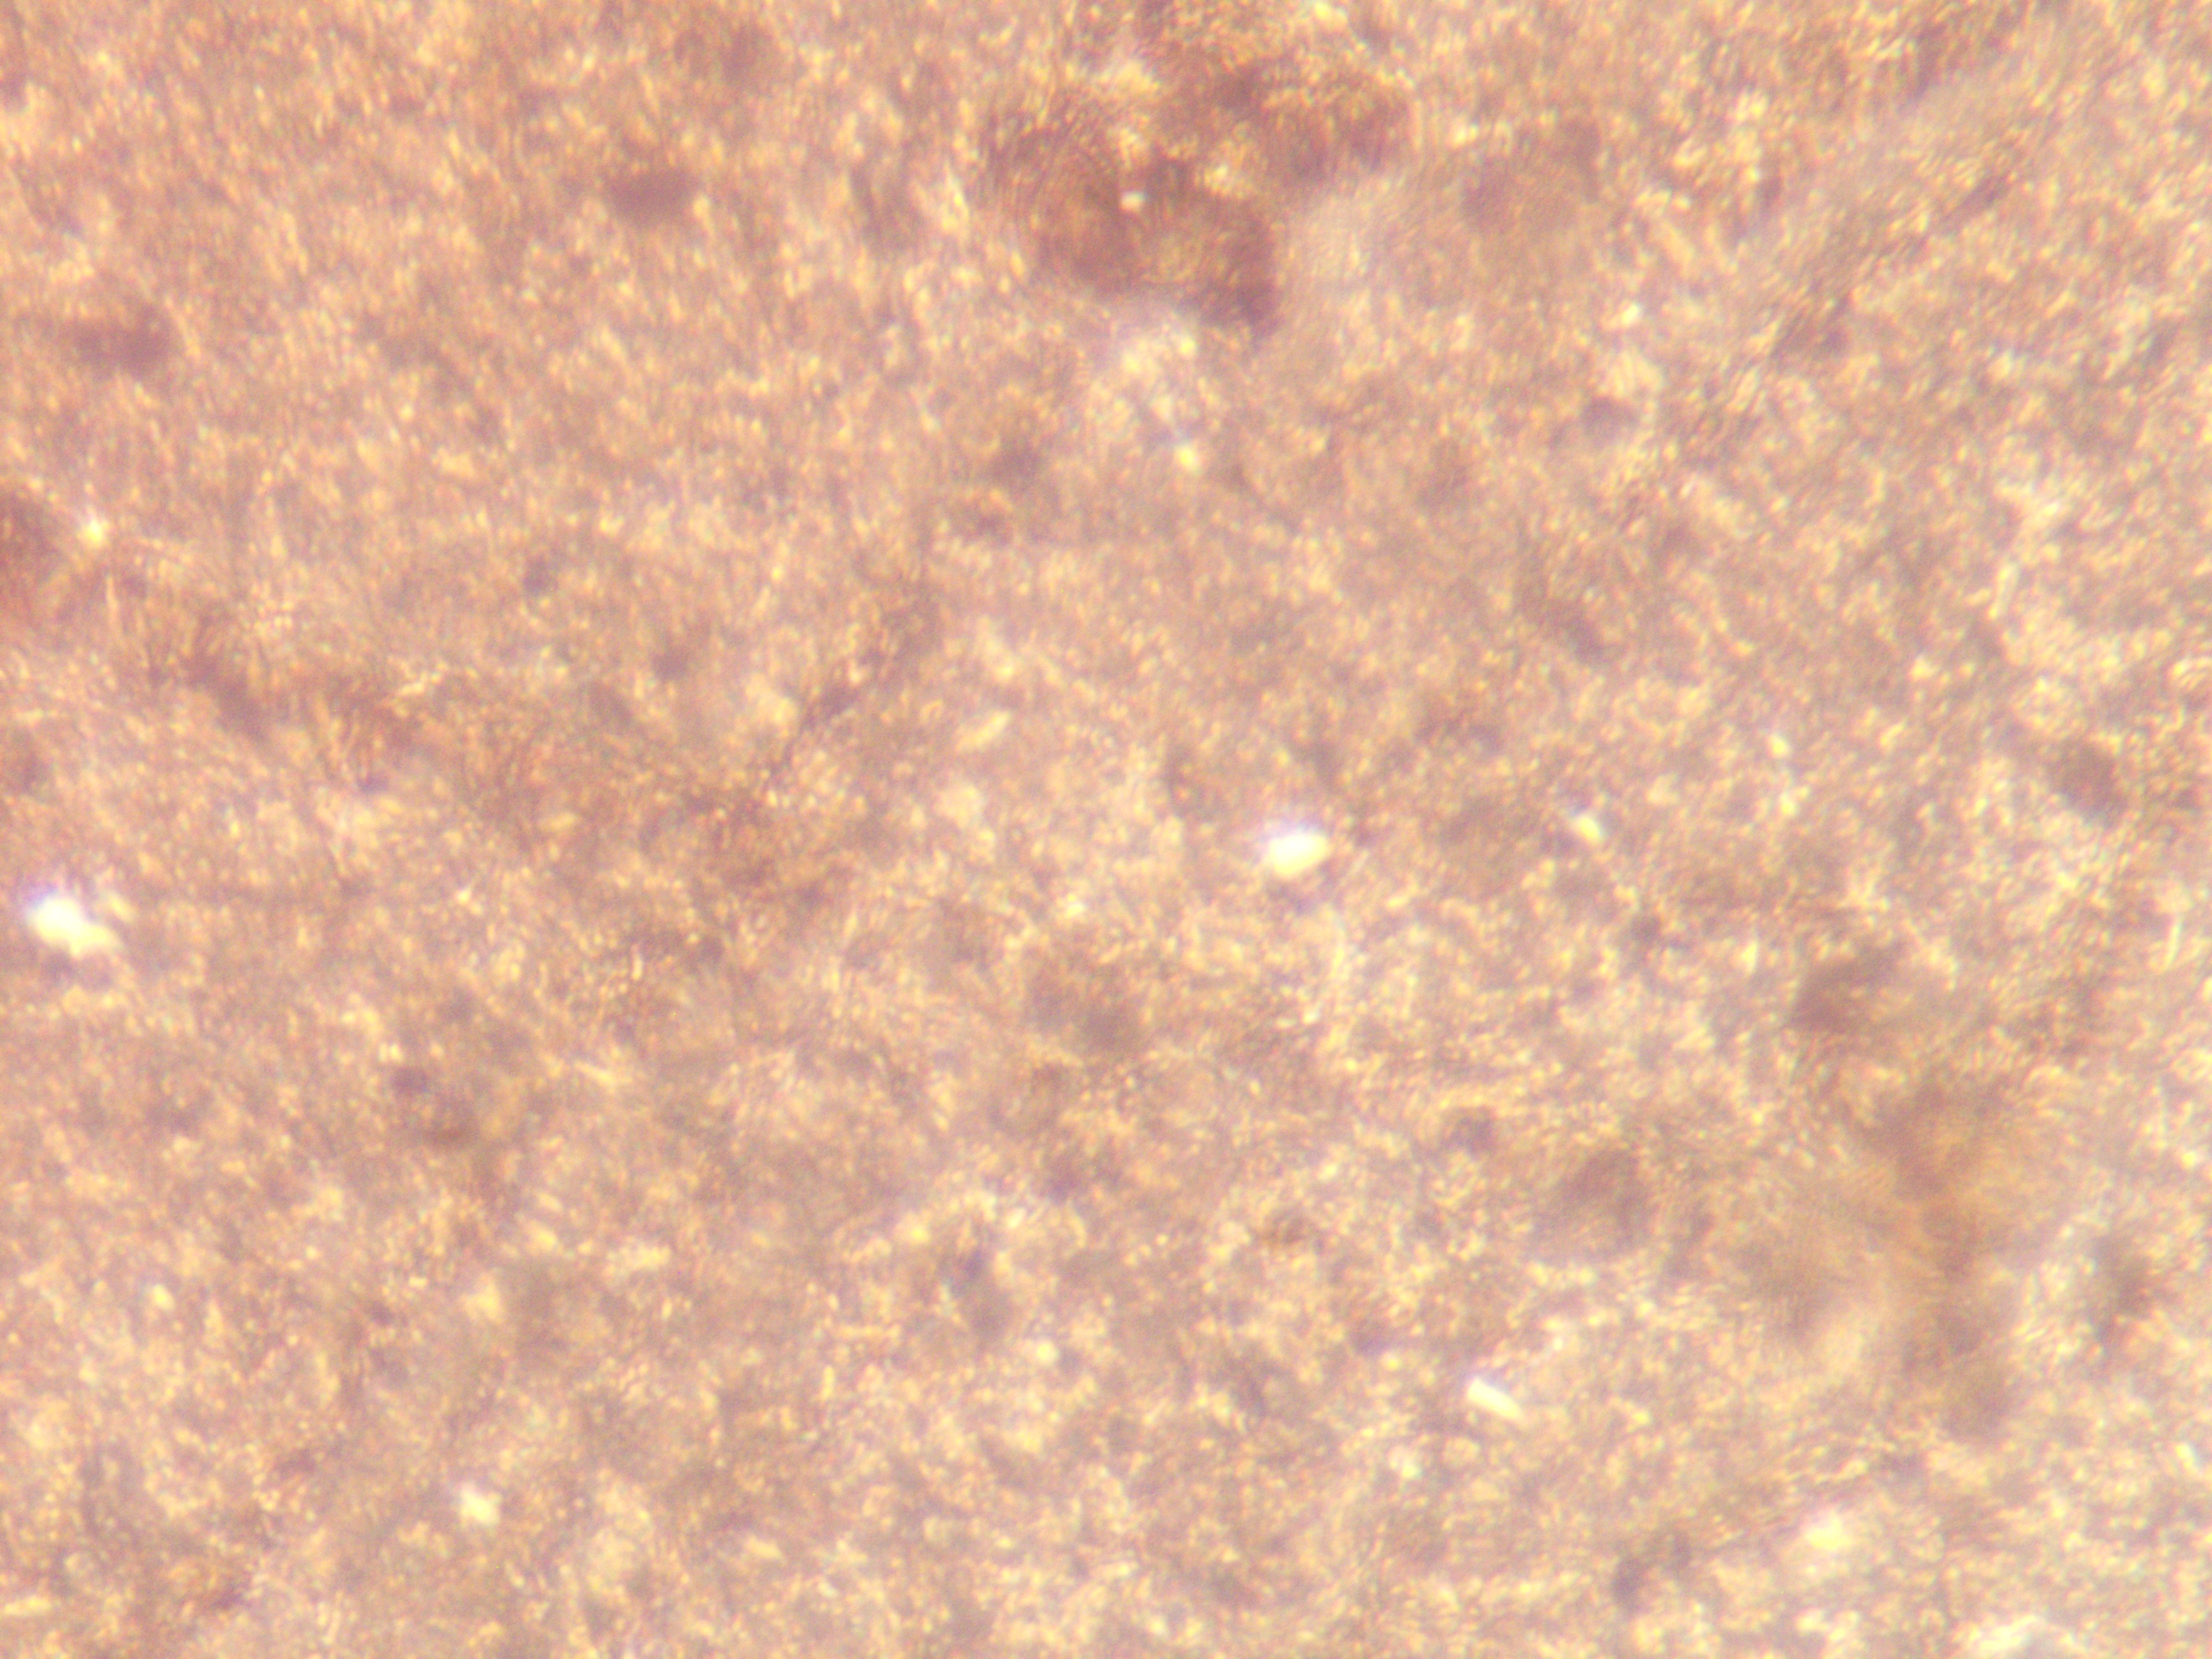
\includegraphics[width=50mm]{26-500.jpg}}
        \ffigbox[50mm]{\caption{26}}{
\includegraphics[width=50mm]{5.png}}
            
    \end{floatrow}

\end{figure}

14.\#27,T12钢1100°C水淬+低温回火

如图,二十七,二十八,其结构为不同黑色树枝状的(针状的)马氏体相互交错,白色部分为残余的奥氏体,
白色部分占比较小,结构中马氏体较多。
\begin{figure}[!ht]
    \begin{floatrow}
        \ffigbox[50mm]{\caption{27-200}}{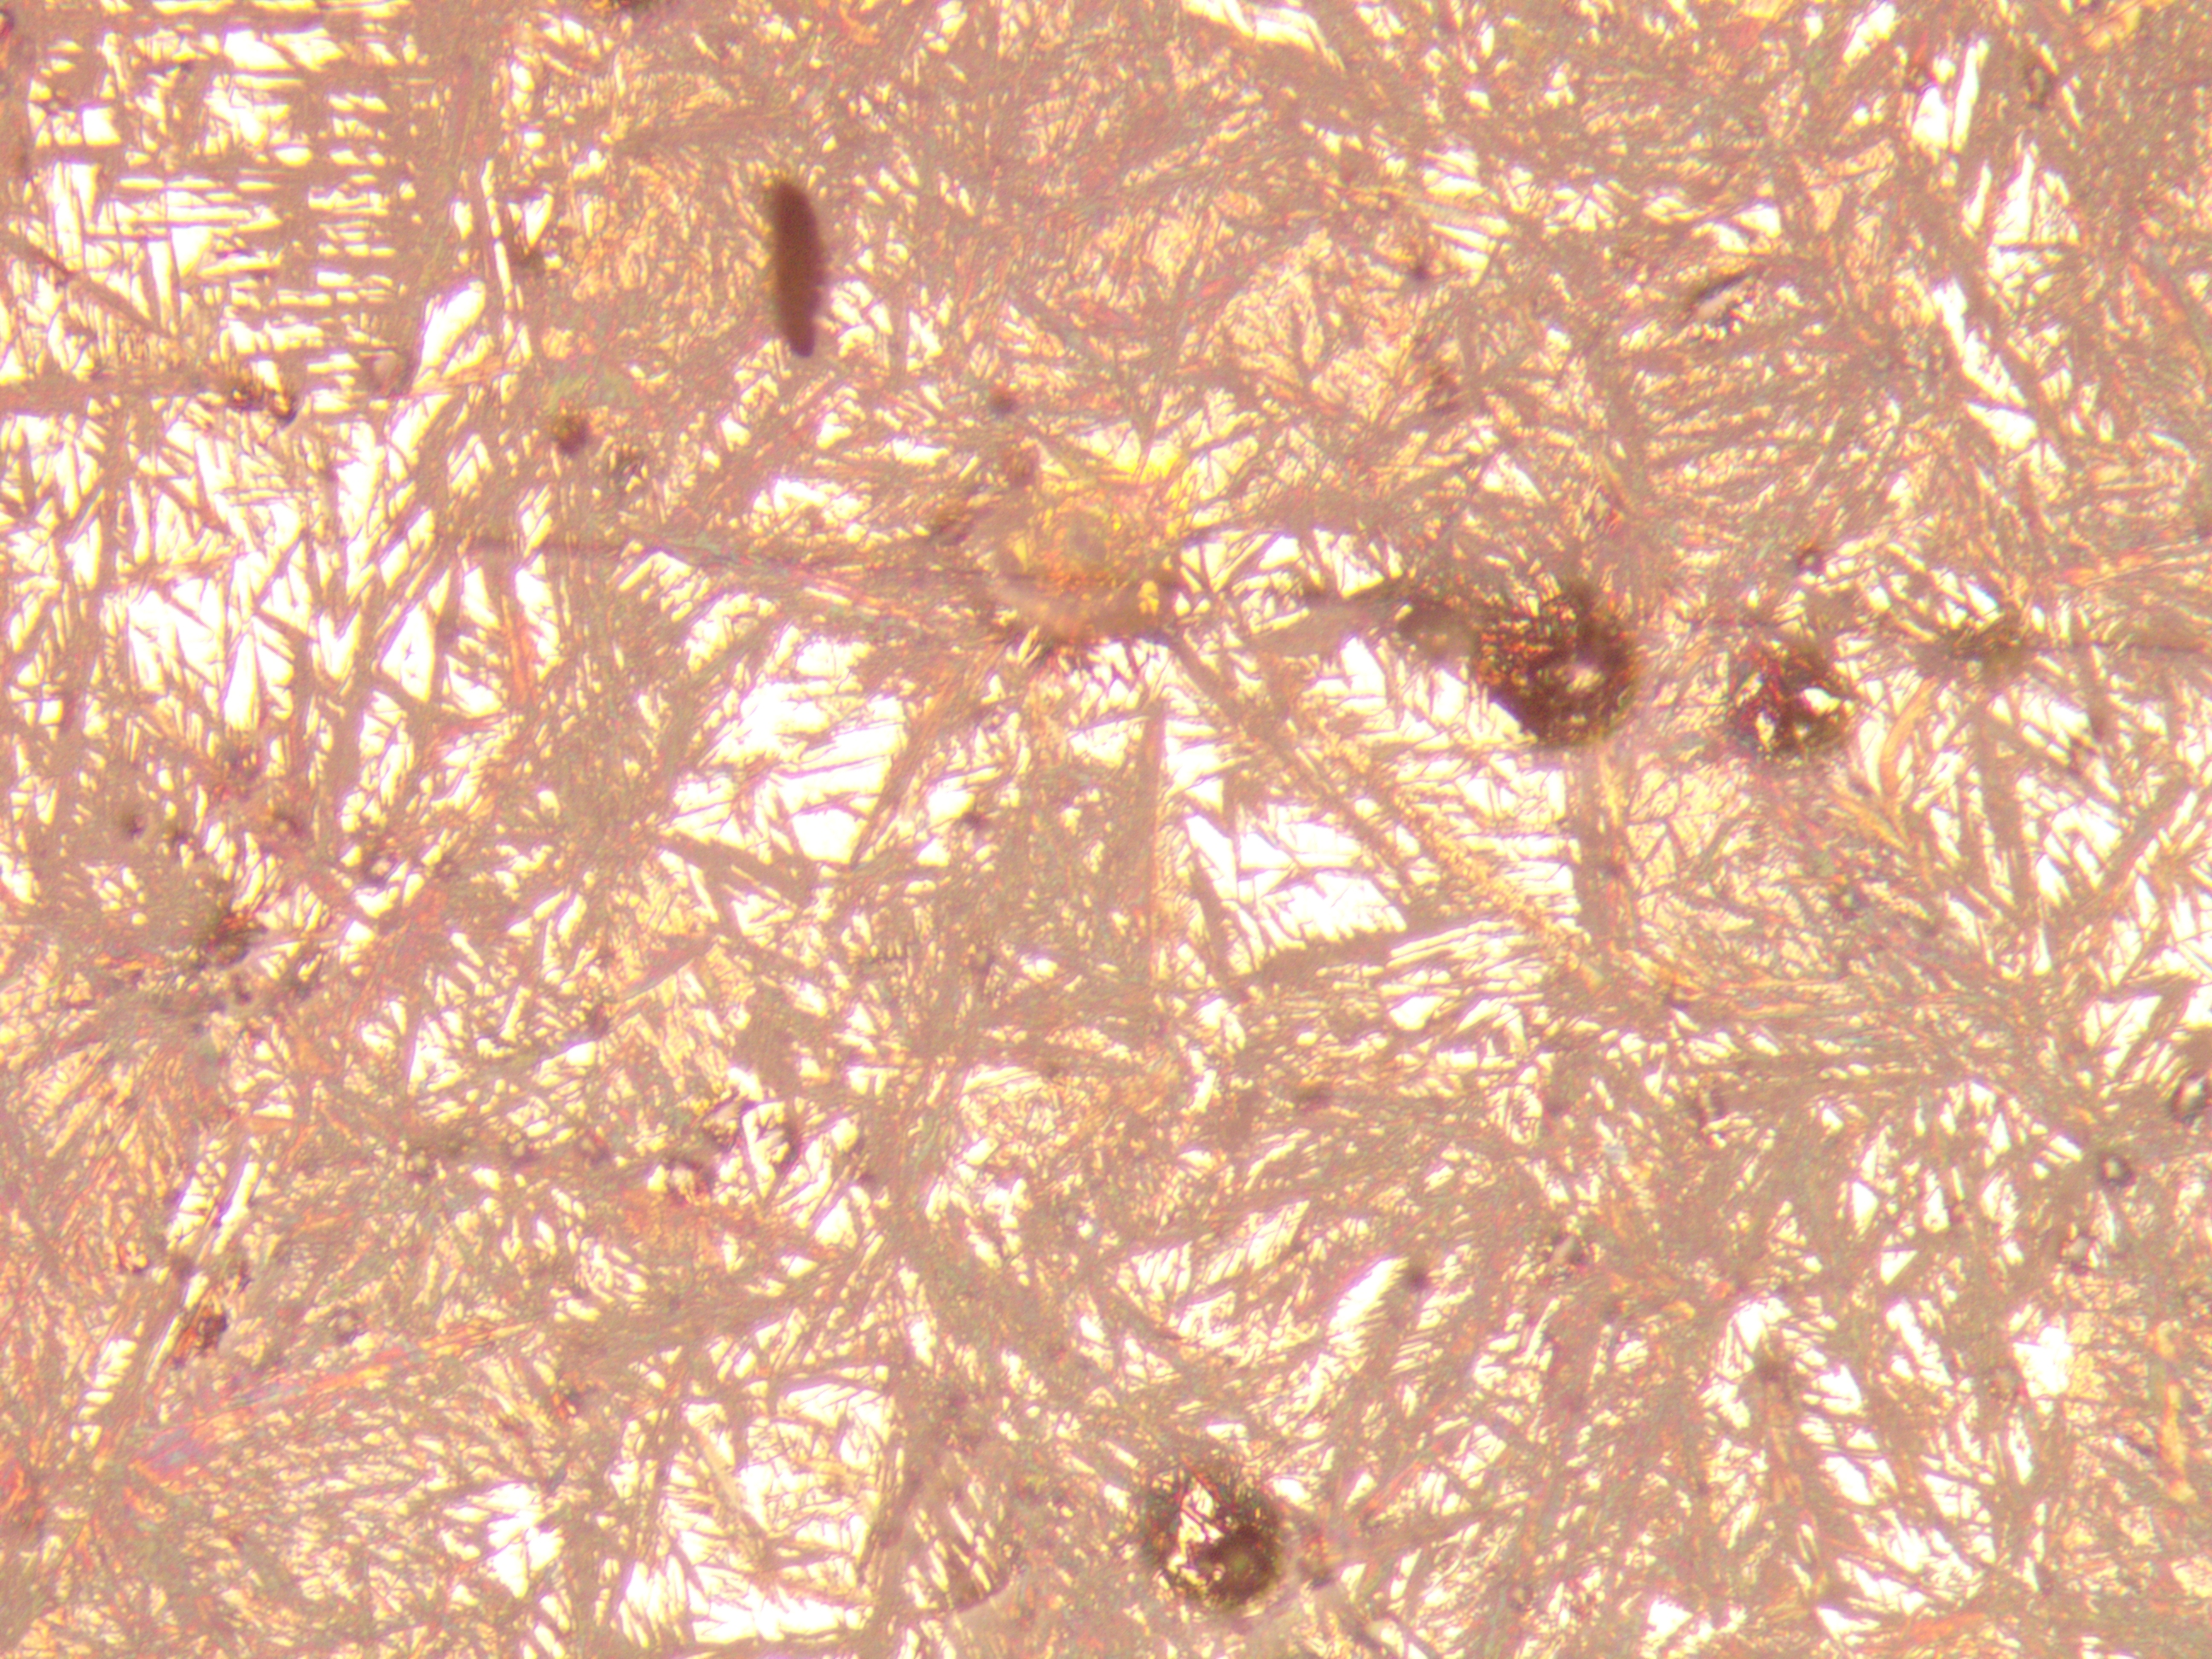
\includegraphics[width=50mm]{27-200.jpg}}
        \ffigbox[50mm]{\caption{27-500}}{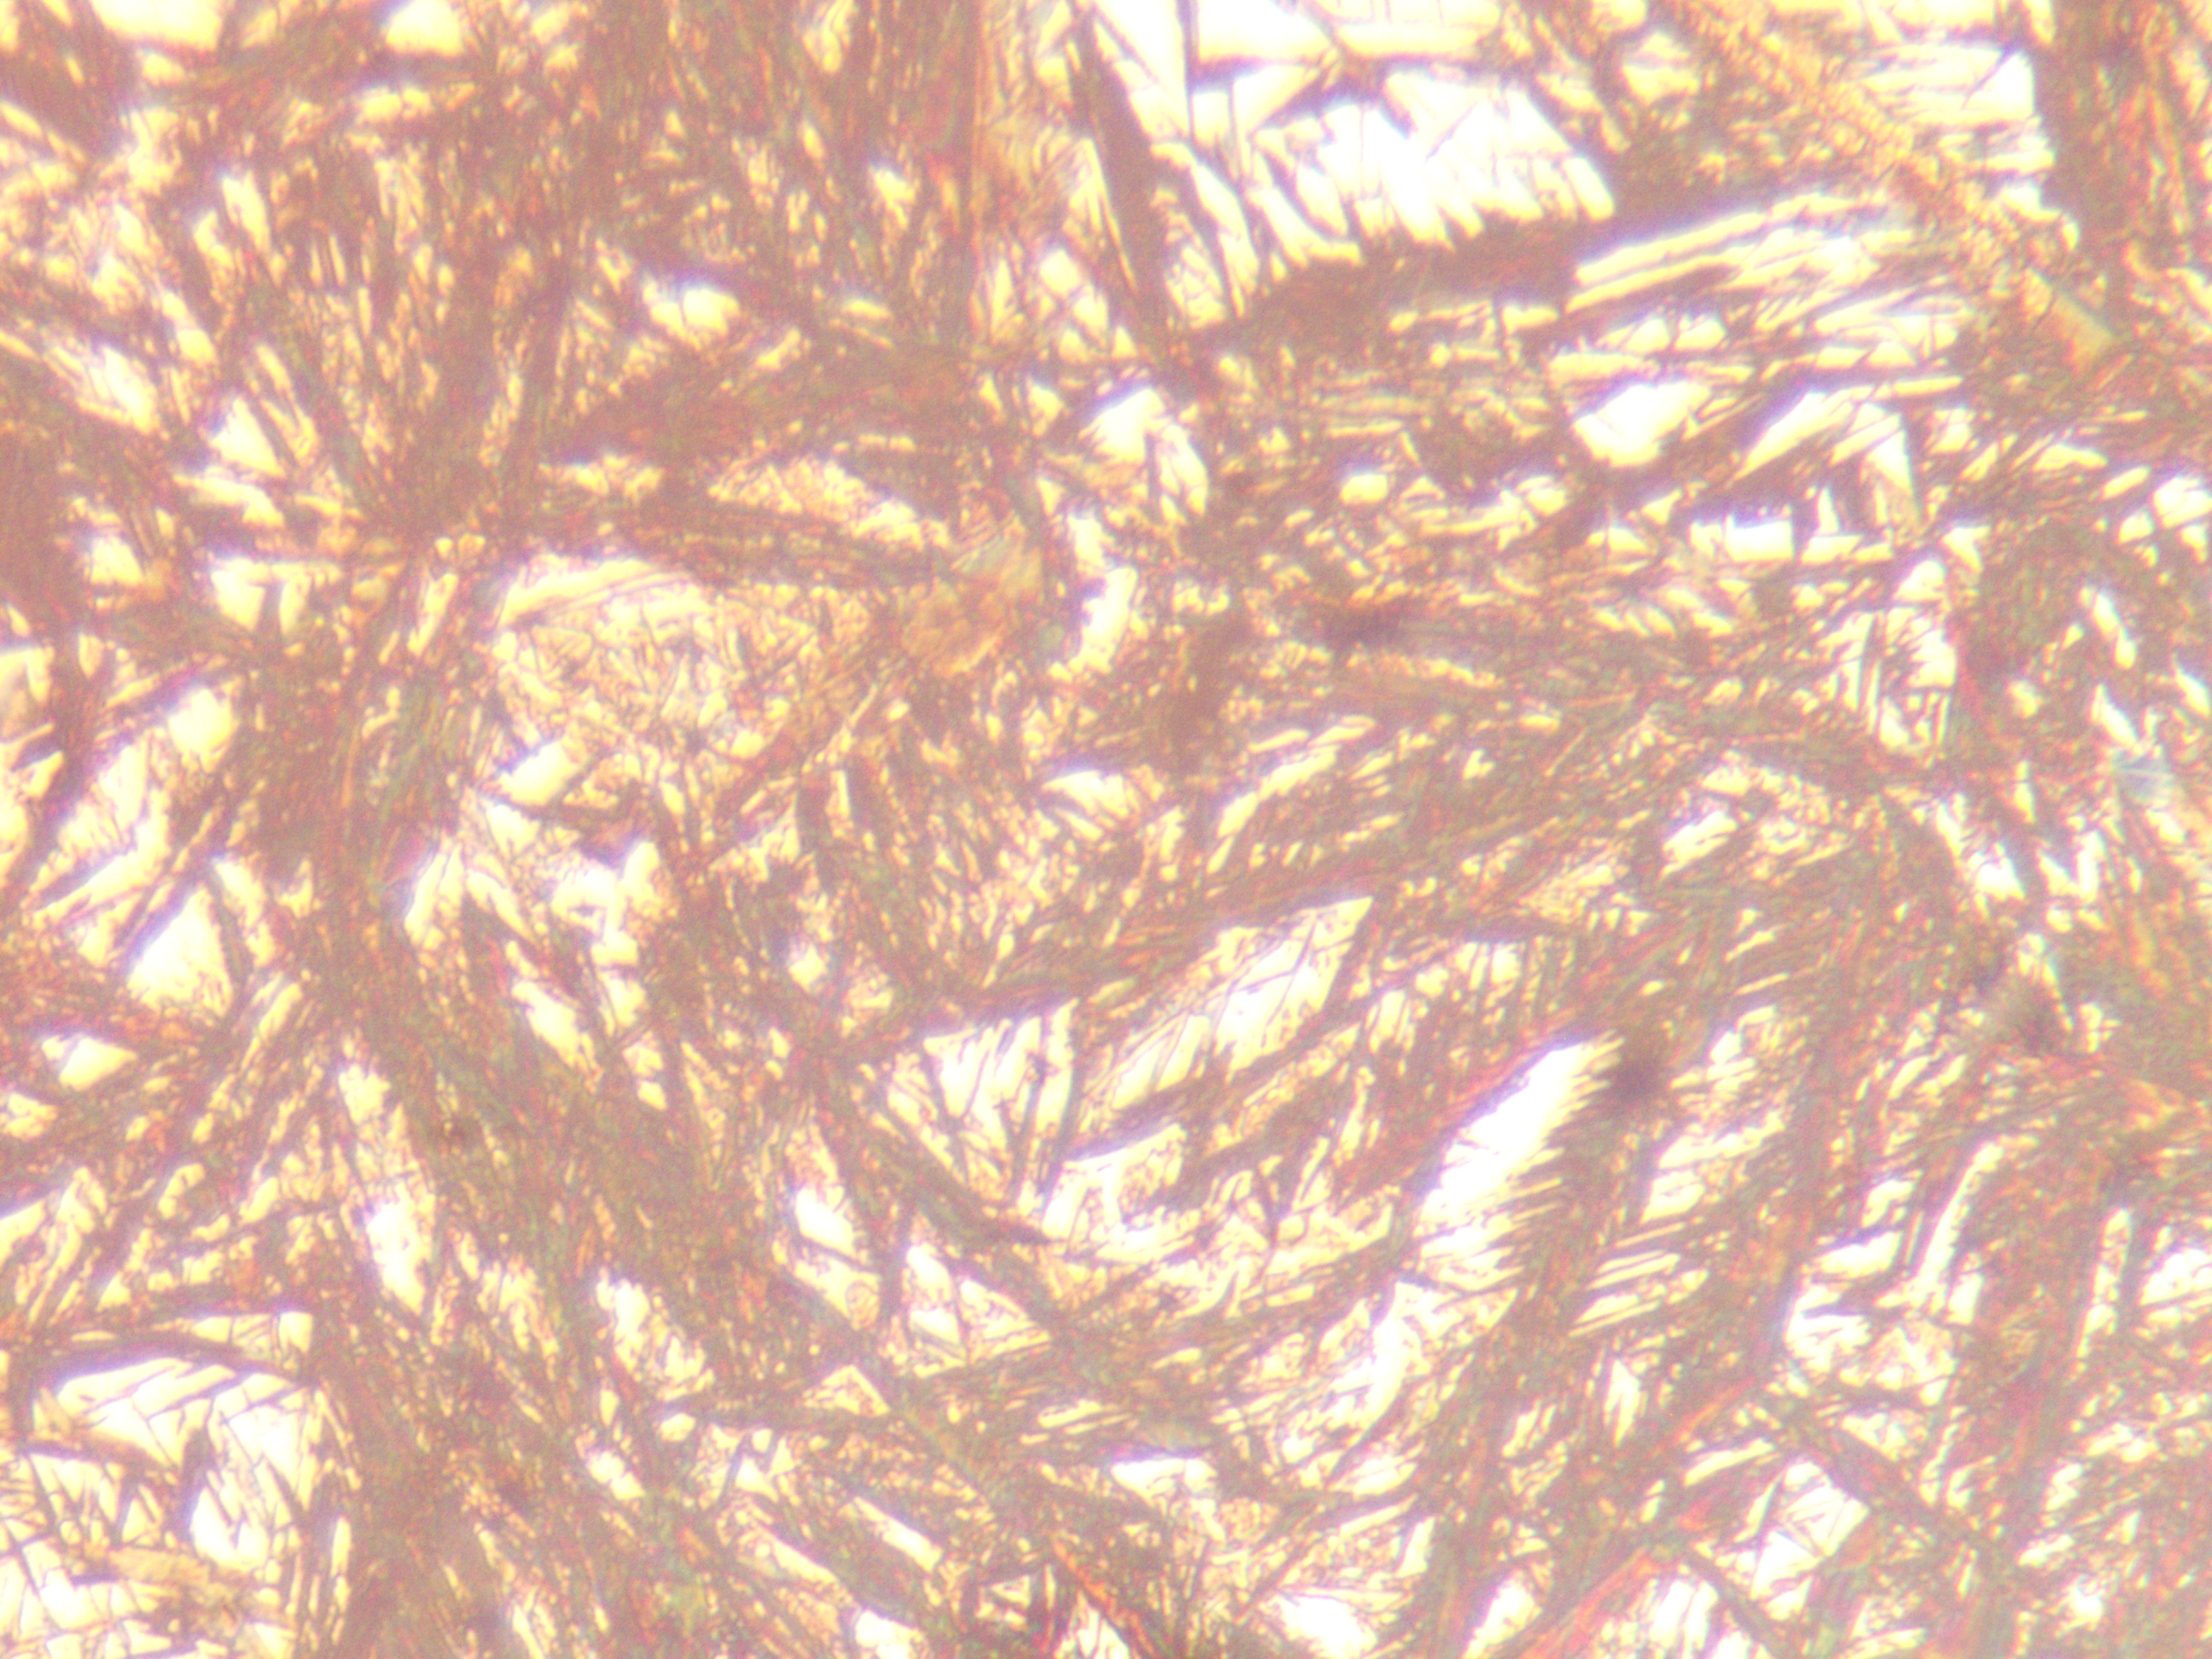
\includegraphics[width=50mm]{27-500.jpg}}
        \ffigbox[50mm]{\caption{27}}{
\includegraphics[width=50mm]{5.png}}
            
    \end{floatrow}

\end{figure}



一、不同热处理工艺条件下试样的组织变化

结合下图,我们可以分析得到:
45钢中温淬火得到的结构是马氏体,而高温淬火时得到的是珠光体;
中温回火得到的是回火屈氏体,而高温回火结构便改变为回火索氏体。
T12钢球化退火生成的是回火马氏体和Fe3C,而同样低温回火的条件下,
低温水淬得到的是回火马氏体+碳化物的组合,
高温水淬则变成了马氏体与奥氏体的结合,不同热处理工艺下样品组织变化极大。

\begin{center}
    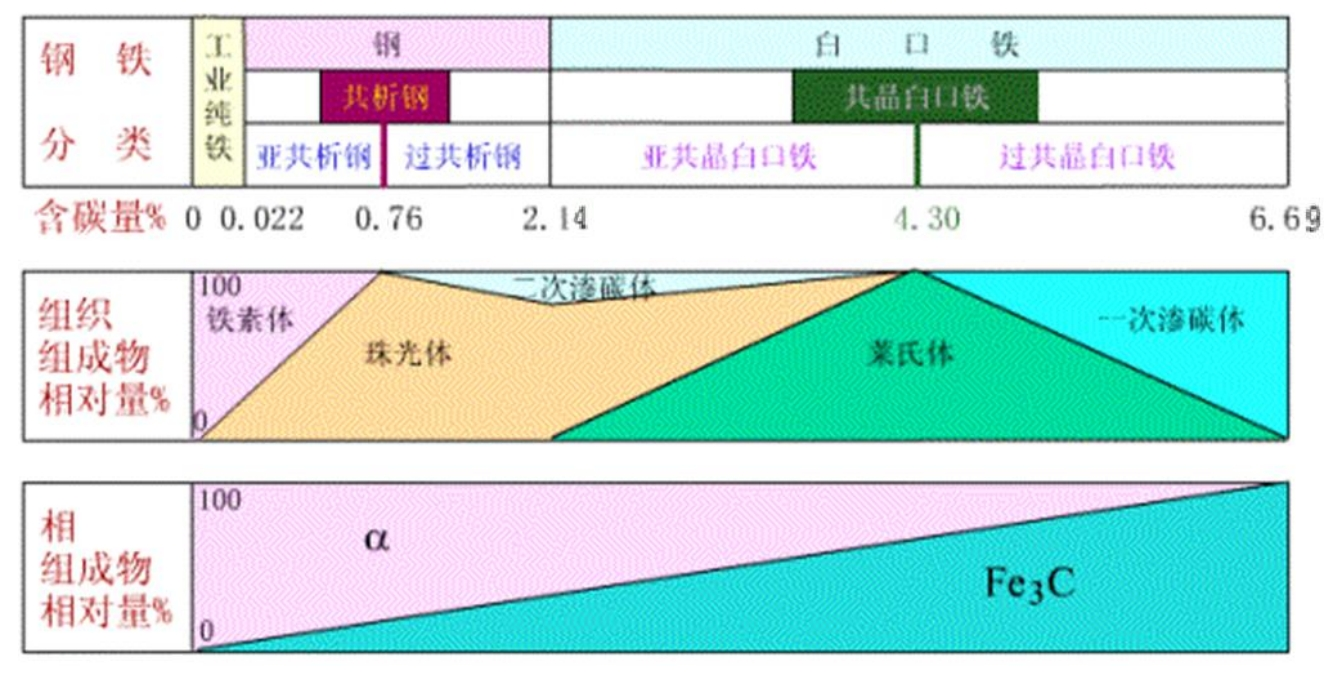
\includegraphics[width=400pt]{3.png} 
\end{center}

\section*{【思考题】}
一、(1)一般步骤如下
    \begin{enumerate}
        \item 检查。检查金相显微镜,试样等完好没有损坏,不会再使用的过程中,影响后续使用。显微镜的各部分连接正常,所有旋钮正常,并且将载物台归位。
        \item 调整。先使用低倍镜,先通过调节显微镜粗调手轮缓慢调节物镜与载物台的距离,使物镜与样品之间达到观察所需最小距离,能看到物像,通过调节孔径光阑、视场光阑,得到最佳观察亮度。
        \item 移动。移动在舞台,将想要观察的部分至于视野的中央。
        \item 用低倍镜观察,而后转换高倍镜观察,观察时转换细准焦,使得物像清晰。
        \item 在观察结束后,用粗调手轮增大物镜与载物台之间的距离,而后取下试样。调节载物台纵向和横向移动手柄将载物台对中(初始状态),关闭显微镜电源,待冷却后盖上防尘罩。
    \end{enumerate}

    (2)注意事项
    \begin{enumerate}
        \item 所有涉及移动物镜的操作均要小心损坏物镜。
        \item 手、试样等不能触碰物镜、目镜镜头,以免损坏镜头。
        \item 使用显微镜时需注意光源的亮度,过强的光源会导致样品过度曝光,影响观察效果。使用完毕后,要及时关闭显微镜的电源以延长设备寿命。
        \item 不得直接用手移动载物台。
        \item 观察结束后要先增大物镜与载物台之间的距离,才能进行取下试样的操作。
        \item 每一次离开显微镜工位转入其他操作前,转换物镜座至低倍物镜(初始状态),调节载物台
        纵向和横向移动手柄将载物台对中(初始状态),关闭显微镜电源。
        \item 使用显微镜前必须保证手、样品干燥整洁,不得残留有水、腐蚀剂、抛光膏等。    
    \end{enumerate}  

二、共有五种

\begin{enumerate}
    \item 一次渗碳体:直接由液态结晶出来的渗碳体,形态是白色长条状。在含碳量大于2.11\%的铁碳合金中才能见到。
    \item 二次渗碳体:由奥氏体超出碳溶解度而析出来的,形态是沿着奥氏体晶界分布,成网状。常可见于过共析钢退火平衡组织、亚共晶铸铁冷却时析出等。
    \item 三次渗碳体:由铁素体超出碳溶解度而析出来的,形态是沿着铁素体晶界分布,由于含量太少,形不成网状,以短棒状分布于铁素体晶界。
    \item 共晶渗碳体:共晶反应生成的渗碳体,与奥氏体共同形成莱氏体,形态白色条状,大小不一。
    \item 共析渗碳体:共析反应生成的渗碳体,与铁素体共同形成珠光体,形态一般是白色片状。
\end{enumerate}

三、冷却曲线如下

\begin{figure}[!ht]
    \begin{floatrow}
        \ffigbox[60mm]{\caption{铁碳合金冷却曲线}}{
\includegraphics[width=100mm]{5.png}}
    \end{floatrow}

\end{figure}

组织变化过程:
    \begin{enumerate}
        \item 按照铁碳相图从最高温度开始降温,合金先按匀晶转变结晶出δ固溶体,冷到1495℃,
        δ固溶体中碳的质量分数达到0.09\%,
        液相中碳质量分数达到0.53\%,
        此时液相与δ溶体发生包晶转变,由于合金中碳的质量分数大于0.17\%,
        所以包晶转变终了以后,还有过剩的液相存在。
        \item 然后,剩余的液相又以匀晶转变继续结晶出奥氏体,冷到,合金全部由碳质量分数为0.45\%的奥氏体组成。
        \item 体系中剩余的液相继续凝固生成奥氏体,合金变为单相奥氏体。
        \item 开始在奥氏体晶界上析出铁素体,称为先共析铁素体,随着温度的下降,
        铁素体量不断增多,而奥氏体量不断减少。铁素体中碳质量分数沿GP线变化,
        而剩余奥氏体中碳的含量则沿GS线变化。当温度接近5点时(727℃),铁素体的成分接近P点。
        \item ,当温度到达727℃时,体系发生共析转变,奥氏体转变为珠光体.
        \item 先共析铁素体将析出三次渗碳体,但其数量很少,可以忽略。
        故该合金的室温组织仍为铁素体与珠光体。
    \end{enumerate}


四、含碳量对铁碳合金的组织和性能的影响

强度:随着含碳量的增加,铁碳合金中软而韧的铁素体含量逐渐减少,硬而脆的渗碳体含量逐渐增多,材料的强度、硬度不断提高,塑性、韧性不断降低。
当含碳量超过0.9\%后,由于网状渗碳体的出现,割裂了珠光体基体的联系,材料的强度随含碳量的增加不断降低。
含碳量小于0.77\%时,随含碳量的增加,珠光体量增多,强
度增加;含碳量在0.77$\sim$ 0.9\%时,由于网状二次Fe3C的出现,强度增加变慢;含碳量达到0.90\%
时,强度出现峰值;含碳量大于0.90\%时,二次Fe3C沿晶界形成完整的网,强度迅速降低,随
着碳质量分数的进一步增加,强度不断下降;

硬度:硬度主要取决于组织组成物的硬度和质量分数,随含碳量的增加,合金的硬度呈直
线关系增大。

塑性:铁碳合金的塑性全部由铁素体(F)提供,渗碳体(Fe3C)是极脆的相,没有塑性。
所以随含碳量的增大,铁素体(F)量不断减少时,合金的塑性连续下降。

韧性:韧性对组织十分敏感,随着合金含碳量的增加,韧性下降。当出现网状二次Fe3C时,
韧性急剧下降,下降趋势要大于塑性。
\end{document}

